% Options for packages loaded elsewhere
\PassOptionsToPackage{unicode}{hyperref}
\PassOptionsToPackage{hyphens}{url}
\documentclass[
]{article}
\usepackage{xcolor}
\usepackage{amsmath,amssymb}
\setcounter{secnumdepth}{5}
\usepackage{iftex}
\ifPDFTeX
  \usepackage[T1]{fontenc}
  \usepackage[utf8]{inputenc}
  \usepackage{textcomp} % provide euro and other symbols
\else % if luatex or xetex
  \usepackage{unicode-math} % this also loads fontspec
  \defaultfontfeatures{Scale=MatchLowercase}
  \defaultfontfeatures[\rmfamily]{Ligatures=TeX,Scale=1}
\fi
% \usepackage{lmodern}
\ifPDFTeX\else
  % xetex/luatex font selection
\fi
% Use upquote if available, for straight quotes in verbatim environments
\IfFileExists{upquote.sty}{\usepackage{upquote}}{}
\IfFileExists{microtype.sty}{% use microtype if available
  \usepackage[]{microtype}
  \UseMicrotypeSet[protrusion]{basicmath} % disable protrusion for tt fonts
}{}
\makeatletter
\@ifundefined{KOMAClassName}{% if non-KOMA class
  \IfFileExists{parskip.sty}{%
    \usepackage{parskip}
  }{% else
    \setlength{\parindent}{0pt}
    \setlength{\parskip}{6pt plus 2pt minus 1pt}}
}{% if KOMA class
  \KOMAoptions{parskip=half}}
\makeatother
\usepackage{color}
\usepackage{fancyvrb}
\newcommand{\VerbBar}{|}
\newcommand{\VERB}{\Verb[commandchars=\\\{\}]}
\DefineVerbatimEnvironment{Highlighting}{Verbatim}{commandchars=\\\{\}}
% Add ',fontsize=\small' for more characters per line
\newenvironment{Shaded}{}{}
\newcommand{\AlertTok}[1]{\textcolor[rgb]{1.00,0.00,0.00}{\textbf{#1}}}
\newcommand{\AnnotationTok}[1]{\textcolor[rgb]{0.38,0.63,0.69}{\textbf{\textit{#1}}}}
\newcommand{\AttributeTok}[1]{\textcolor[rgb]{0.49,0.56,0.16}{#1}}
\newcommand{\BaseNTok}[1]{\textcolor[rgb]{0.25,0.63,0.44}{#1}}
\newcommand{\BuiltInTok}[1]{\textcolor[rgb]{0.00,0.50,0.00}{#1}}
\newcommand{\CharTok}[1]{\textcolor[rgb]{0.25,0.44,0.63}{#1}}
\newcommand{\CommentTok}[1]{\textcolor[rgb]{0.38,0.63,0.69}{\textit{#1}}}
\newcommand{\CommentVarTok}[1]{\textcolor[rgb]{0.38,0.63,0.69}{\textbf{\textit{#1}}}}
\newcommand{\ConstantTok}[1]{\textcolor[rgb]{0.53,0.00,0.00}{#1}}
\newcommand{\ControlFlowTok}[1]{\textcolor[rgb]{0.00,0.44,0.13}{\textbf{#1}}}
\newcommand{\DataTypeTok}[1]{\textcolor[rgb]{0.56,0.13,0.00}{#1}}
\newcommand{\DecValTok}[1]{\textcolor[rgb]{0.25,0.63,0.44}{#1}}
\newcommand{\DocumentationTok}[1]{\textcolor[rgb]{0.73,0.13,0.13}{\textit{#1}}}
\newcommand{\ErrorTok}[1]{\textcolor[rgb]{1.00,0.00,0.00}{\textbf{#1}}}
\newcommand{\ExtensionTok}[1]{#1}
\newcommand{\FloatTok}[1]{\textcolor[rgb]{0.25,0.63,0.44}{#1}}
\newcommand{\FunctionTok}[1]{\textcolor[rgb]{0.02,0.16,0.49}{#1}}
\newcommand{\ImportTok}[1]{\textcolor[rgb]{0.00,0.50,0.00}{\textbf{#1}}}
\newcommand{\InformationTok}[1]{\textcolor[rgb]{0.38,0.63,0.69}{\textbf{\textit{#1}}}}
\newcommand{\KeywordTok}[1]{\textcolor[rgb]{0.00,0.44,0.13}{\textbf{#1}}}
\newcommand{\NormalTok}[1]{#1}
\newcommand{\OperatorTok}[1]{\textcolor[rgb]{0.40,0.40,0.40}{#1}}
\newcommand{\OtherTok}[1]{\textcolor[rgb]{0.00,0.44,0.13}{#1}}
\newcommand{\PreprocessorTok}[1]{\textcolor[rgb]{0.74,0.48,0.00}{#1}}
\newcommand{\RegionMarkerTok}[1]{#1}
\newcommand{\SpecialCharTok}[1]{\textcolor[rgb]{0.25,0.44,0.63}{#1}}
\newcommand{\SpecialStringTok}[1]{\textcolor[rgb]{0.73,0.40,0.53}{#1}}
\newcommand{\StringTok}[1]{\textcolor[rgb]{0.25,0.44,0.63}{#1}}
\newcommand{\VariableTok}[1]{\textcolor[rgb]{0.10,0.09,0.49}{#1}}
\newcommand{\VerbatimStringTok}[1]{\textcolor[rgb]{0.25,0.44,0.63}{#1}}
\newcommand{\WarningTok}[1]{\textcolor[rgb]{0.38,0.63,0.69}{\textbf{\textit{#1}}}}
\usepackage{longtable,booktabs,array}
\newcounter{none} % for unnumbered tables
\usepackage{calc} % for calculating minipage widths
% Correct order of tables after \paragraph or \subparagraph
\usepackage{etoolbox}
\makeatletter
\patchcmd\longtable{\par}{\if@noskipsec\mbox{}\fi\par}{}{}
\makeatother
% Allow footnotes in longtable head/foot
\IfFileExists{footnotehyper.sty}{\usepackage{footnotehyper}}{\usepackage{footnote}}
\makesavenoteenv{longtable}
\usepackage{graphicx}
\makeatletter
\newsavebox\pandoc@box
\newcommand*\pandocbounded[1]{% scales image to fit in text height/width
  \sbox\pandoc@box{#1}%
  \Gscale@div\@tempa{\textheight}{\dimexpr\ht\pandoc@box+\dp\pandoc@box\relax}%
  \Gscale@div\@tempb{\linewidth}{\wd\pandoc@box}%
  \ifdim\@tempb\p@<\@tempa\p@\let\@tempa\@tempb\fi% select the smaller of both
  \ifdim\@tempa\p@<\p@\scalebox{\@tempa}{\usebox\pandoc@box}%
  \else\usebox{\pandoc@box}%
  \fi%
}
% Set default figure placement to htbp
\def\fps@figure{htbp}
\makeatother
\setlength{\emergencystretch}{3em} % prevent overfull lines
\providecommand{\tightlist}{%
  \setlength{\itemsep}{0pt}\setlength{\parskip}{0pt}}
\usepackage[]{natbib}
\bibliographystyle{plainnat}
\makeatletter
\@ifpackageloaded{subcaption}{}{\usepackage{subcaption}}
\@ifpackageloaded{caption}{}{\usepackage{caption}}
\captionsetup[subfigure]{margin=0.5em}
\AtBeginDocument{%
\renewcommand*\figurename{Figure}
\renewcommand*\tablename{Table}
}
\AtBeginDocument{%
\renewcommand*\listfigurename{List of Figures}
\renewcommand*\listtablename{List of Tables}
}
\newcounter{pandoccrossref@subfigures@footnote@counter}
\newenvironment{pandoccrossrefsubfigures}{%
\setcounter{pandoccrossref@subfigures@footnote@counter}{0}
\begin{figure}\centering%
\gdef\global@pandoccrossref@subfigures@footnotes{}%
\DeclareRobustCommand{\footnote}[1]{\footnotemark%
\stepcounter{pandoccrossref@subfigures@footnote@counter}%
\ifx\global@pandoccrossref@subfigures@footnotes\empty%
\gdef\global@pandoccrossref@subfigures@footnotes{{##1}}%
\else%
\g@addto@macro\global@pandoccrossref@subfigures@footnotes{, {##1}}%
\fi}}%
{\end{figure}%
\addtocounter{footnote}{-\value{pandoccrossref@subfigures@footnote@counter}}
\@for\f:=\global@pandoccrossref@subfigures@footnotes\do{\stepcounter{footnote}\footnotetext{\f}}%
\gdef\global@pandoccrossref@subfigures@footnotes{}}
\@ifpackageloaded{float}{}{\usepackage{float}}
\floatstyle{ruled}
\@ifundefined{c@chapter}{\newfloat{codelisting}{h}{lop}}{\newfloat{codelisting}{h}{lop}[chapter]}
\floatname{codelisting}{Listing}
\newcommand*\listoflistings{\listof{codelisting}{List of Listings}}
\makeatother
\usepackage{bookmark}
\IfFileExists{xurl.sty}{\usepackage{xurl}}{} % add URL line breaks if available
\urlstyle{same}
% fallback for those not using the hyperref driver hyperxmp:
\makeatletter
\@ifundefined{xmpquote}{\newcommand{\xmpquote}[1]{#1}}{}
\makeatother
\hypersetup{
  colorlinks=true,linkcolor=red,urlcolor=red,citecolor=red,anchorcolor=red,filecolor=red,
  pdfcreator={LaTeX via pandoc}}

\author{}
\date{}

\IfFileExists{seqsplit.sty}{\usepackage{seqsplit}}{\newcommand{\seqsplit}[1]{#1}}
\protected\def\breakseq#1{\seqsplit{#1}}
\protected\def\breaktt#1{\begingroup\ttfamily\seqsplit{#1}\endgroup}
\title{A Living Meta-Analysis of the Modafinil Literature}
\author{Daniel Ari Friedman\\\footnotesize{Active Inference Institute}\\\footnotesize{\texttt{daniel@activeinference.institute}}\\\footnotesize{\href{https://orcid.org/0000-0001-6232-9096}{ORCID: 0000-0001-6232-9096}} \\ \footnotesize{DOI: \href{https://doi.org/10.5281/zenodo.20931964}{10.5281/zenodo.20931964}}}
\date{\today}

% Core mathematics
\usepackage{amsmath}
\usepackage{amssymb}
\usepackage{amsfonts}
\usepackage{amsthm}

% Document layout
\usepackage[margin=1.8cm]{geometry}
\usepackage{float}
\usepackage{graphicx}
\usepackage[section]{placeins}  % Constrain floats to their section
\renewcommand{\floatpagefraction}{0.7}  % Require 70% fill for float-only pages
\renewcommand{\topfraction}{0.9}        % Allow large top floats

% Tables
\usepackage{booktabs}
\usepackage{longtable}
\usepackage{array}
\usepackage{multirow}

% Code listings
\usepackage{listings}

% Typography and formatting
\usepackage{microtype}
\usepackage{xcolor}

% Cross-references and citations (hyperref loaded by other packages with [unicode]; set options only)
\hypersetup{colorlinks=true,linkcolor=red,citecolor=red,urlcolor=red}
\usepackage[capitalise,noabbrev]{cleveref}
% NOTE: natbib is auto-injected by Pandoc via --natbib (which also writes
% \bibliographystyle{plainnat}). Do not re-declare \usepackage{natbib} here
% or LaTeX will error with "Option clash for package natbib".

% Figure caption formatting
\usepackage{caption}
\usepackage{subcaption}

% Algorithm typesetting
\usepackage[ruled,vlined]{algorithm2e}

% Custom commands for domain notation
\newcommand{\FEP}{\textsc{fep}}
\newcommand{\AIF}{\textsc{aif}}
\newcommand{\KL}{\mathrm{KL}}
\newcommand{\E}{\mathbb{E}}
\newcommand{\F}{\mathcal{F}}

% NMF and topic modeling notation
\newcommand{\matW}{\mathbf{W}}  % NMF document-topic matrix
\newcommand{\matH}{\mathbf{H}}  % NMF topic-term matrix
\newcommand{\matV}{\mathbf{V}}  % NMF document-term matrix
\newcommand{\tfidf}{\text{TF-IDF}}
\newcommand{\cagr}{\text{CAGR}}
\newcommand{\score}{\operatorname{score}}
\newcommand{\corpusvar}[1]{\texttt{\{\{#1\}\}}}
\newcommand{\scoreH}[1]{\text{score}(H_{#1})}
\newcommand{\EBM}{\textsc{ebm}}
\newcommand{\VFE}{\mathcal{F}_{\text{VFE}}}
\newcommand{\RBM}{\textsc{rbm}}

% Assertion and evidence notation
\newcommand{\supports}{\mathrel{\text{supports}}}
\newcommand{\contradicts}{\mathrel{\text{contradicts}}}
\newcommand{\neutral}{\mathrel{\text{neutral}}}

% Domain taxonomy shorthands
\newcommand{\domA}{\text{A}}
\newcommand{\domB}{\text{B}}
\newcommand{\domC}{\text{C}}

% Evidence-score and growth metrics
\newcommand{\EFE}{\mathbf{G}}       % Evidence-score matrix
\newcommand{\doubling}{t_d}         % Doubling time
\newcommand{\meangrowth}{\bar{g}}   % Mean year-over-year growth rate

% Corpus and scoring notation
\newcommand{\Nstart}{N_{\text{start}}}  % Publication count in first year
\newcommand{\Nend}{N_{\text{end}}}      % Publication count in last year
\newcommand{\SH}{S(H)}                  % Supporting assertions for H
\newcommand{\CH}{C(H)}                  % Contradicting assertions for H
\newcommand{\AH}{A(H)}                  % All assertions for H

% Tool and project shorthands
\newcommand{\nanopub}{\textsc{np}}      % Nanopublication shorthand
\newcommand{\ollama}{\textsc{Ollama}}   % Ollama LLM server
\newcommand{\pymdp}{\textsc{pymdp}}     % pymdp library

% Network and graph operators
\DeclareMathOperator{\PageRank}{PageRank}  % PageRank operator

\begin{document}

\begin{titlepage}
\centering
\vspace*{2cm}
{\LARGE\bfseries A Living Meta-Analysis of the Modafinil Literature\par}
\vspace{0.75em}
{\large Multi-Engine Retrieval, De-duplication, Embeddings, and Bibliometrics for a Single Search Term\par}
\vfill
\makeatletter
{\@author\par}
\vspace{1em}
{\@date\par}
\makeatother
\vfill
\end{titlepage}
\thispagestyle{empty}
\tableofcontents
\newpage


\section{Abstract}\label{abstract}

Manual synthesis cannot keep pace with a fast-growing research
literature, and ad-hoc reviews bind no evidence to a reproducible
pipeline. We present a configurable, reproducible meta-analysis
framework that takes a single search term and produces a complete
quantitative portrait of its literature. For this instance the term is
\textbf{Modafinil}. The pipeline dispatches across 7 literature engines
(arXiv, OpenAlex, Semantic Scholar, Crossref, PubMed, SovietRxiv, and
ChinaRxiv), each degrading gracefully to a skipped source when an API
key or the network is unavailable, then merges and de-duplicates records
by a canonical identifier hierarchy (DOI \(>\) arXiv ID \(>\) Semantic
Scholar ID \(>\) OpenAlex ID \(>\) title digest) into a corpus of
\(N = 2302\) records spanning 2000--2026 (26 years). Records are
classified into a configurable 6-bucket subfield taxonomy (Clinical
Sleep, Cognition, Pharmacology, Psychiatry, Safety, and Neuroscience);
the largest subfield is \textbf{Clinical Sleep} (64.3\% of the
classified corpus). The corpus grows at a compound annual rate of 3.45\%
(mean year-over-year growth 6.3\%, doubling time 11.3 years), peaking in
2025 with 112 records.

Non-negative matrix factorization extracts 5 latent topics over a
500-feature vocabulary, offline deterministic embeddings place every
title, abstract, and (when available) full text in a shared vector
space, and citation-network analysis exposes the corpus's internal
structure (8,772 intra-corpus edges across 2204 nodes, 1377 communities,
graph density 0.18\%). Of 38,802 total outgoing references, 22.6\%
resolve to another record inside the corpus. Abstract coverage stands at
55.5\%, open-access status is known for 14.4\% of records, and 40.9\%
have a direct PDF link. An optional, LLM-gated knowledge-graph stage
scores the 6 hypotheses explored against the evidence. This run produced
18 publication-quality figures.

Every domain-specific value in this manuscript --- the search term,
keyword set, engine roster, subfield taxonomy, and hypotheses --- is
injected from a single configuration file and the pipeline's own
outputs; re-targeting the configuration re-targets the entire paper. The
result is a reusable architecture for \emph{living literature reviews}:
continuously re-runnable, evidence-bound syntheses for any topic.

\textbf{Keywords:} modafinil, meta-analysis, literature retrieval,
bibliometrics, record de-duplication, full-text mining, document
embeddings, citation network, topic modeling, entity extraction,
wakefulness, cognitive enhancement, reproducible research

\newpage

\section{Introduction}\label{introduction}

The scholarly literature on any active topic grows faster than any
individual can read. A researcher entering a field needs to know how
large it is, how fast it is growing, what sub-areas compose it, which
works anchor its citation structure, what language and concepts recur,
and which claims the field actually tests. Answering those questions by
hand is slow, unrepeatable, and binds no number to evidence. Systematic
reviews, while the gold standard for evidence synthesis, are
labour-intensive and become stale between updates --- the Cochrane
review cycle, for instance, targets a two-year refresh interval that
many fields outpace \citep{page2021prisma}. Bibliometric dashboards
(Scopus, Web of Science, Dimensions) offer breadth but no reproducible
link from a reported statistic to a regenerable artifact, and they do
not frame or test domain-specific hypotheses.

This project is a \textbf{configurable, reproducible meta-analysis
template}. It takes one search term and produces a quantitative portrait
of that term's literature, with every reported number traceable to a
committed artifact and regenerable by re-running the pipeline. The
bundled instance targets \textbf{Modafinil}, a wakefulness-promoting
agent with a large, multi-disciplinary literature spanning clinical
sleep medicine, cognitive neuroscience, pharmacology, psychiatry, and
safety research; pointing the configuration at a different term
re-targets the whole analysis with no code change.

\subsection{Research Questions}\label{research-questions}

The pipeline is designed around four research questions (RQs) that a
researcher entering the field would ask:

\begin{enumerate}
\def\labelenumi{\arabic{enumi}.}
\item
  \textbf{RQ1 --- Field size and growth.} How large is the literature on
  Modafinil, how fast is it growing, and when did it peak? The corpus of
  \(N = 2302\) records spanning 2000--2026 answers this directly, with a
  compound annual growth rate of 3.45\% and a peak in 2025.
\item
  \textbf{RQ2 --- Subfield composition.} What sub-areas compose the
  literature, and what is their relative weight? A configurable 6-bucket
  taxonomy (Clinical Sleep, Cognition, Pharmacology, Psychiatry, Safety,
  and Neuroscience) classifies every record, with \textbf{Clinical
  Sleep} the largest bucket at 64.3\%.
\item
  \textbf{RQ3 --- Topical and linguistic structure.} What language and
  concepts recur, and what latent topics cross-cut the keyword taxonomy?
  TF-IDF over a 500-feature vocabulary feeds non-negative matrix
  factorization, which extracts 5 latent topics. The top vocabulary
  terms are: modafinil, treatment, study, effects, patients, results,
  sleep, used, use, drug, studies, clinical, mg, using, placebo,
  cognitive, associated, effect, however, disorder.
\item
  \textbf{RQ4 --- Citation geometry and evidence landscape.} Which works
  anchor the citation structure, how self-contained is the retrieved
  slice, and which claims does the field test? The citation network of
  2204 nodes and 8,772 edges (22.6\% reference resolution rate) exposes
  hubs, authorities, and communities, while 6 configured hypotheses
  frame the evidence landscape.
\end{enumerate}

\subsection{Contributions}\label{contributions}

The pipeline contributes an end-to-end, domain-agnostic workflow:

\begin{enumerate}
\def\labelenumi{\arabic{enumi}.}
\item
  \textbf{Multiple-engine retrieval with graceful degradation.} Records
  are gathered from 7 independent engines (arXiv, OpenAlex, Semantic
  Scholar, Crossref, PubMed, SovietRxiv, and ChinaRxiv). An engine with
  no API key or no network reports a \emph{skipped} status; the run
  completes from whatever engines remain plus a committed offline
  corpus. For this live run, OpenAlex contributed the largest share of
  records, followed by Crossref and PubMed; Semantic Scholar was
  rate-limited (HTTP 429) and returned zero records without aborting the
  pipeline.
\item
  \textbf{Record de-duplication.} Heterogeneous records are merged by a
  canonical identifier hierarchy, keeping the most complete version of
  each work. Of 2302 retrieved records, 2248 carry DOIs, 932 carry
  OpenAlex IDs, and 1 carry arXiv IDs.
\item
  \textbf{Descriptive and bibliometric analysis.} Counts by year, venue,
  and author; growth metrics (CAGR 3.45\%, doubling time 11.3 years); a
  configurable 6-bucket subfield classification; topic models; and a
  citation network with 1377 communities.
\item
  \textbf{Language, entity, and embedding analysis.} Keyphrase and
  entity extraction and offline deterministic document embeddings over
  titles, abstracts, and full text. The TF-IDF vocabulary of 500
  features captures the lexical landscape.
\item
  \textbf{Optional hypothesis evidence.} An LLM-gated knowledge-graph
  stage scores the 6 configured hypotheses explored against the corpus.
\end{enumerate}

Because the writing itself is token-injected from configuration and
pipeline outputs, the manuscript is part of the reproducible artifact
rather than a separate hand-authored narrative. Every number, table, and
figure reference in this document traces to a committed, regenerable
file under \texttt{output/}.

\newpage

\section{Methods Overview}\label{methods-overview}

The pipeline is a sequence of deterministic stages, each reading the
previous stage's committed artifacts and writing its own. Business logic
lives in tested \texttt{src/} modules; the numbered \texttt{scripts/}
are thin orchestrators that wire I/O, configuration loading, logging,
and stage sequencing. The architecture follows the thin orchestrator
pattern: no computational logic resides in scripts.

\subsection{Pipeline Stages}\label{pipeline-stages}

\begin{enumerate}
\def\labelenumi{\arabic{enumi}.}
\item
  \textbf{Retrieval} (\breaktt{01\_literature\_search.py}) --- dispatch
  the configured query across 7 engines (arXiv, OpenAlex, Semantic
  Scholar, Crossref, PubMed, SovietRxiv, and ChinaRxiv), merge, and
  de-duplicate into \texttt{corpus.jsonl}. Each engine is an isolated
  adapter exposing a uniform
  \texttt{search(query)\ -\textgreater{}\ list{[}Paper{]}} interface;
  engines that are keyless need no credentials, while Semantic Scholar
  uses a key when present. SovietRxiv and ChinaRxiv share a unified API
  with an optional \texttt{X-API-Email} header for the polite rate-limit
  pool (300/min vs 30/min anonymous).
\item
  \textbf{Meta-analysis} (\breaktt{02\_meta\_analysis\_pipeline.py}) ---
  subfield classification, temporal metrics, TF-IDF, non-negative matrix
  factorization topics, and the citation network. This stage reads
  \texttt{corpus.jsonl} and emits
  \breaktt{subfield\_classification.json},
  \breaktt{temporal\_analysis.json}, \texttt{tfidf\_data.json},
  \texttt{topics.json}, \breaktt{citation\_network.json}, and
  \breaktt{citation\_graph.gml}.
\item
  \textbf{Knowledge graph} (\breaktt{03\_build\_knowledge\_graph.py},
  optional/LLM-gated) --- extract assertions and score the 6 configured
  hypotheses. Outputs \breaktt{nanopublications.jsonl},
  \breaktt{hypothesis\_scores.json}, and
  \breaktt{assertion\_summary.json}.
\item
  \textbf{Figures} (\breaktt{04\_generate\_figures.py}) --- render 18
  publication-ready visualizations from the analysis JSON outputs. All
  figures use a colourblind-safe palette (Wong 2011), high-contrast
  labels at \(\geq 16\)pt, and a headless matplotlib backend (Agg).
\item
  \textbf{Injection} (\breaktt{05\_inject\_variables.py}) --- compute
  manuscript variables from the artifacts above and substitute them into
  these Markdown sections. An unresolved placeholder is a hard error,
  not a silent gap.
\item
  \textbf{Fulltext assessment} (\breaktt{06\_fulltext\_assessment.py})
  --- report abstract coverage (55.5\%), open-access status (14.4\%),
  and PDF availability (40.9\%) across the corpus.
\end{enumerate}

\subsection{Reproducibility Model}\label{reproducibility-model}

The system runs \textbf{offline and deterministically} by default: a
committed synthetic seed corpus drives every stage with fixed seeds
(seed = 42 for NMF, SVD, and graph layouts), so re-running produces
byte-identical outputs. A live run with engines enabled and credentials
supplied replaces the seed corpus with real records --- as in this
instance, which retrieved 2302 live records. The template is
domain-agnostic: the search term, query, keyword set, subfield taxonomy,
and hypotheses all come from \breaktt{manuscript/config.yaml}.

\subsection{Configuration Surface}\label{configuration-surface}

A single \breaktt{manuscript/config.yaml} controls:

\begin{itemize}
\tightlist
\item
  \textbf{Search parameters}: term, query string, per-engine queries,
  relevance keywords, start year, max results, resume/clear behaviour
\item
  \textbf{Engine toggles}: arXiv, OpenAlex, Semantic Scholar, Crossref,
  PubMed, SovietRxiv, ChinaRxiv (each independently enabled or disabled)
\item
  \textbf{SovietRxiv/ChinaRxiv settings}: optional \texttt{api\_email}
  for the polite pool, \texttt{source} filter (\texttt{russiarxiv} or
  \texttt{chinaxiv})
\item
  \textbf{Full-text download}: opt-in Unpaywall resolution with
  \texttt{unpaywall\_email}
\item
  \textbf{Embeddings}: method (\texttt{tfidf\_svd} or
  \texttt{transformer}), dimensionality, max features
\item
  \textbf{Knowledge graph}: checkpoint interval, LLM model, base URL,
  temperature, max tokens
\item
  \textbf{Hypothesis definitions}: 6 named hypotheses with scope labels
\item
  \textbf{Subfield taxonomy}: 6 buckets, each with a keyword list
\item
  \textbf{Paper metadata}: title, authors, DOI, keywords, license,
  repository URL
\end{itemize}

\newpage

\section{Retrieval and
De-duplication}\label{retrieval-and-de-duplication}

Retrieval dispatches the configured query across 7 independent
literature engines (arXiv, OpenAlex, Semantic Scholar, Crossref, PubMed,
SovietRxiv, and ChinaRxiv). Each engine is an isolated adapter exposing
a uniform \texttt{search(query)\ -\textgreater{}\ list{[}Record{]}}
interface; engines that are keyless --- arXiv, OpenAlex
\citep{priem2022openalex}, Crossref \citep{hendricks2020crossref},
PubMed/Entrez \citep{sayers2022entrez}, SovietRxiv / RussiaRxiv, and
ChinaRxiv --- need no credentials, while Semantic Scholar
\citep{kinney2023semantic} uses a key when present. SovietRxiv is a
translated archive of Soviet-era scientific preprints sourced from
Math-Net.Ru and CyberLeninka \citep{sovietrxiv}; ChinaRxiv serves
translated Chinese preprints from ChinaXiv via the same unified API.
Both retain original-language PDFs alongside each translation, and their
polite rate-limit pool (300/min vs 30/min anonymous) is activated by an
optional \texttt{X-API-Email} header. Optional full-text resolution
queries Unpaywall \citep{piwowar2018state} for open-access locations.
\textbf{Multiple dispatch degrades gracefully}: an engine that is
disabled in the configuration, lacks a required key, or cannot reach the
network returns a \emph{skipped} status, and the run completes from the
remaining engines plus the committed offline corpus.

\subsection{Engine Details}\label{engine-details}

Each engine adapter follows a uniform contract: a module-level API URL
constant, a pure \texttt{\_parse\_*} parser function, and a
\texttt{search\_*} entry point with pagination, retry, and graceful
error handling. All functions accept an injectable \texttt{base\_url}
parameter for hermetic testing with \breaktt{pytest-httpserver} --- no
engine hardcodes its URL inside the function body.

{\def\LTcaptype{none} % do not increment counter
\begin{longtable}[]{@{}
  >{\raggedright\arraybackslash}p{(\linewidth - 8\tabcolsep) * \real{0.2000}}
  >{\raggedright\arraybackslash}p{(\linewidth - 8\tabcolsep) * \real{0.2000}}
  >{\raggedright\arraybackslash}p{(\linewidth - 8\tabcolsep) * \real{0.2000}}
  >{\raggedright\arraybackslash}p{(\linewidth - 8\tabcolsep) * \real{0.2000}}
  >{\raggedright\arraybackslash}p{(\linewidth - 8\tabcolsep) * \real{0.2000}}@{}}
\toprule\noalign{}
\begin{minipage}[b]{\linewidth}\raggedright
Engine
\end{minipage} & \begin{minipage}[b]{\linewidth}\raggedright
Rate limit
\end{minipage} & \begin{minipage}[b]{\linewidth}\raggedright
Pagination
\end{minipage} & \begin{minipage}[b]{\linewidth}\raggedright
Auth
\end{minipage} & \begin{minipage}[b]{\linewidth}\raggedright
Records (this run)
\end{minipage} \\
\midrule\noalign{}
\endhead
\bottomrule\noalign{}
\endlastfoot
arXiv & 3s between requests & 100/page, offset & Keyless & Sparse \\
Semantic Scholar & 1 req/s (unauth.) & 100/page, offset & Optional key &
Skipped (429) \\
OpenAlex & Polite pool (mailto) & 200/page, cursor & Keyless & 1,000 \\
Crossref & Polite pool (mailto) & 1,000/page, offset & Keyless &
1,000 \\
PubMed & NCBI usage policy & retstart/retmax & Keyless & 986 \\
SovietRxiv & 30/min (300/min polite) & 1--100/page, cursor &
\texttt{X-API-Email} & 0 \\
ChinaRxiv & 30/min (300/min polite) & 1--100/page, cursor &
\texttt{X-API-Email} & 0 \\
\end{longtable}
}

SovietRxiv and ChinaRxiv returned zero records for the modafinil query,
which is expected: the Soviet-era archive covers mathematics, physics,
and engineering preprints, while ChinaXiv covers Chinese scientific
preprints, and neither domain has substantial modafinil literature. The
engines dispatched correctly, queried the live API, and returned empty
result sets without error --- confirming graceful degradation.

\subsection{Canonical Identifier
Hierarchy}\label{canonical-identifier-hierarchy}

Heterogeneous records are reconciled by a \textbf{canonical identifier
hierarchy} --- DOI \(>\) arXiv ID \(>\) Semantic Scholar ID \(>\)
OpenAlex ID \(>\) a stable digest of the normalized title. When two
records share a canonical identifier they are merged, keeping the
version with the most complete metadata (a count of non-None optional
fields). The DOI is normalized: case-folded, resolver-prefix stripped,
so the same paper returned by two engines under case/format-variant DOIs
merges. For this run, 2248 records carry DOIs, 932 carry OpenAlex IDs,
and 1 carry arXiv IDs. The de-duplicated corpus for this run holds
\(N = 2302\) records published across 2000--2026.

\subsection{Relevance Filtering}\label{relevance-filtering}

After de-duplication, a relevance filter drops papers whose title and
abstract contain none of the configured relevance keywords (modafinil,
armodafinil, provigil, wakefulness, narcolepsy, cognitive enhancement,
alertness, sleep deprivation, vigilance, eugeroic). Keywords are matched
case-insensitively; an empty keyword list is treated as no filter to
avoid silently wiping the corpus. A year filter then excludes papers
published before the configured start year (2000).

\newpage

\section{Full Text, Language, and
Embeddings}\label{full-text-language-and-embeddings}

Beyond bibliographic metadata, the pipeline mines the textual content of
each record. This stage bridges the gap between a bibliographic
inventory and a semantic understanding of the literature.

\subsection{Full-Text Availability}\label{full-text-availability}

An open-access resolver maps each record to a downloadable PDF where one
exists (a known \texttt{pdf\_url}, or an Unpaywall lookup by DOI), and
an opt-in, network-gated downloader fetches it to a deterministic path.
Full-text availability is summarized without requiring any download, so
the offline default still reports coverage. For this run:

\begin{itemize}
\tightlist
\item
  \textbf{Abstract coverage}: 55.5\% of records (1277 of

  \begin{enumerate}
  \def\labelenumi{\arabic{enumi})}
  \setcounter{enumi}{2301}
  \tightlist
  \item
    carry an abstract; 1025 records lack one.
  \end{enumerate}
\item
  \textbf{Open-access status}: 14.4\% of records are open access (331
  records); the remainder are closed or unknown.
\item
  \textbf{PDF availability}: 40.9\% of records (941) have a direct PDF
  link; 940 have a publisher PDF, and 1361 have no full-text source
  available.
\end{itemize}

The identifier coverage for this corpus is: 2248 DOIs, 932 OpenAlex IDs,
and 1 arXiv IDs. DOI coverage dominates, enabling robust cross-engine
de-duplication.

\subsection{Language and Entity
Extraction}\label{language-and-entity-extraction}

Titles, abstracts, and (when present) full text are tokenized and
reduced to keyphrases and named entities by offline, dependency-light
extractors --- no mandatory LLM. Term-frequency statistics drive a
TF-IDF representation over a 500-feature vocabulary. The most frequent
terms in the corpus are: modafinil, treatment, study, effects, patients,
results, sleep, used, use, drug, studies, clinical, mg, using, placebo,
cognitive, associated, effect, however, disorder. These terms reflect
the clinical, pharmacological, and cognitive vocabulary characteristic
of the modafinil literature.

\subsection{Embeddings}\label{embeddings}

Every title, abstract, and full text is embedded into a shared vector
space by a deterministic, offline method --- TF-IDF followed by
truncated SVD, i.e.~latent semantic analysis
\citep{deerwester1990indexing}. The embedding dimensionality is 50
components (configurable via
\breaktt{project\_config.embeddings.n\_components}), and the TF-IDF
vocabulary is capped at 500 features (configurable via
\breaktt{project\_config.embeddings.max\_features}). The embedding is
byte-stable across runs: the same input text always yields identical
vectors, so the derived similarity matrix, nearest-neighbour lists,
clusters, and two-dimensional projection are all reproducible.

An optional transformer backend can be enabled by setting
\breaktt{project\_config.embeddings.method:\ transformer} (requires the
\texttt{embeddings} extra), which upgrades the embedding fidelity
without changing the interface or downstream analysis.

The embeddings support semantic retrieval over the corpus and feed two
visualizations: a PCA two-dimensional projection ((Figure pca
embeddings)) that maps the topical geography of the literature, and a
hierarchical clustering dendrogram ((Figure dendrogram)) that reveals
the similarity structure of the document collection.

\newpage

\section{Bibliometric and Temporal
Analysis}\label{bibliometric-and-temporal-analysis}

Descriptive statistics summarize the corpus along every available axis:
counts by year, venue, and author; citation-count distributions; and
author productivity. Temporal analysis fits the publication time series,
reporting a compound annual growth rate of 3.45\% across 2000--2026 (a
span of 26 years), with a mean year-over-year growth rate of 6.3\% and a
doubling time of 11.3 years. The peak publication year is 2025 with 112
records.

\subsection{Growth Metrics}\label{growth-metrics}

The compound annual growth rate (CAGR) is computed as:

\[
\text{CAGR} = \left(\frac{N_{\text{end}}}{N_{\text{start}}}\right)^{1/(\text{year span})} - 1
\]

where \(N_{\text{start}}\) is the publication count in the first year
(2000) and \(N_{\text{end}}\) is the count in the last year (2026). The
mean year-over-year growth rate \(\bar{g}\) is the arithmetic mean of
annual ratios. The doubling time is
\(t_d = \ln(2) / \ln(1 + \text{CAGR})\). These metrics are stored in
\breaktt{temporal\_analysis.json} and injected into the manuscript at
render time.

\subsection{Subfield Classification}\label{subfield-classification}

Subfield classification assigns each record to one of 6 configurable
buckets (Clinical Sleep, Cognition, Pharmacology, Psychiatry, Safety,
and Neuroscience) by priority-aware keyword matching; the taxonomy is
defined entirely in configuration
(\breaktt{project\_config.subfield\_keywords}). The largest bucket is
\textbf{Clinical Sleep} at 64.3\% of the classified corpus. A
per-subfield temporal breakdown (\breaktt{subfield\_timeline.json})
tracks how each sub-area has grown over time, enabling identification of
emerging or declining research threads.

\subsection{Topic Modeling}\label{topic-modeling}

A TF-IDF term-weighting of titles and abstracts \citep{salton1988term}
feeds non-negative matrix factorization (NMF) \citep{lee1999learning},
implemented with scikit-learn \citep{pedregosa2011scikit}. NMF
decomposes the document-term matrix
\(\mathbf{V} \approx \mathbf{W} \mathbf{H}\), where \(\mathbf{W}\) is
the document-topic matrix and \(\mathbf{H}\) is the topic-term matrix.
The factorization extracts 5 latent topics that cross-cut the keyword
taxonomy. The random seed is fixed at 42 for reproducibility. The
reporting follows established systematic-review practice
\citep{page2021prisma}, with every figure and statistic traceable to a
committed artifact.

\newpage

\section{Optional Knowledge-Graph
Layer}\label{optional-knowledge-graph-layer}

An optional, \textbf{LLM-gated} stage lifts the corpus from
bibliometrics to hypothesis-level evidence. For each record, a local
language model (Ollama, default model \texttt{gemma3:4b}) extracts
structured \emph{assertions} --- each encoding a direction (supports /
contradicts / neutral), a confidence score, and a short natural-language
justification --- against the 6 hypotheses declared in configuration.
Assertions are serialized as RDF-compatible nanopublications
\citep{kuhn2016decentralized} and scored by a citation-weighted evidence
function.

\subsection{Assertion Model}\label{assertion-model}

Each assertion \(a\) encodes:

\begin{itemize}
\tightlist
\item
  \textbf{Direction}: \(\text{supports}\), \(\text{contradicts}\), or
  \(\text{neutral}\) with respect to a hypothesis \(H\)
\item
  \textbf{Confidence}: a score \(c_a \in [0, 1]\) from the LLM
\item
  \textbf{Citation weight}: \(\log(1 + n_{\text{cites}})\), where
  \(n_{\text{cites}}\) is the citation count of the asserting paper
\end{itemize}

The evidence score for hypothesis \(H\) is:

\[
\text{score}(H) = \frac{\sum_{a \in A(H)^+} c_a \cdot \log(1 + n_{\text{cites}}(a)) -
\sum_{a \in A(H)^-} c_a \cdot \log(1 + n_{\text{cites}}(a))}
{\sum_{a \in A(H)} c_a \cdot \log(1 + n_{\text{cites}}(a))}
\]

where \(A(H)^+\) is the set of supporting assertions and \(A(H)^-\) the
contradicting ones. The score ranges from \(-1\) (all evidence
contradicts) to \(+1\) (all evidence supports).

\subsection{Incremental Extraction}\label{incremental-extraction}

Assertion extraction is \textbf{incremental and resumable}: assertions
are appended to \breaktt{nanopublications.jsonl} at configurable
checkpoint intervals (default: 50 papers). On restart, already-processed
papers are skipped automatically, so a long extraction run that is
interrupted can resume without re-processing. The
\breaktt{-\/-clear-assertions} flag discards previous results for a fresh
start.

\subsection{Gating and Defaults}\label{gating-and-defaults}

This stage is entirely optional and never runs in the offline default:
with no language model available it is skipped, and the hypothesis
evidence scores read \emph{pending}. The hypotheses themselves --- their
names and scope --- come from configuration and are reported regardless
of whether the scoring stage has run.

The hypotheses explored in this instance are: H1 Wakefulness Efficacy;
H2 Cognitive Enhancement; H3 Low Abuse Liability; H4 Dopaminergic
Mechanism; H5 Off-label Psychiatric Utility; H6 Tolerability.

\newpage

\section{Visualization and Manuscript
Injection}\label{visualization-and-manuscript-injection}

\subsection{Figure Generation}\label{figure-generation}

Figures are rendered headlessly (matplotlib Agg backend) and
deterministically from the analysis artifacts: subfield distributions,
the publication growth curve, the citation network, topic-term bars, a
term cloud, and embedding projections. All figures use a
colourblind-safe palette (Wong 2011, 8 colours) with high-contrast
labels at \(\geq 16\)pt. This run produced 18 figures at 300 DPI. The
full figure set includes:

\begin{itemize}
\tightlist
\item
  \textbf{Field overview}: field summary and subfield distribution
  ((Figure field summary; Figure subfield distribution))
\item
  \textbf{Temporal}: growth curve and subfield timeline ((Figure growth
  curve; Figure subfield timeline))
\item
  \textbf{Citation network}: network layout and degree distribution
  ((Figure citation network; Figure degree distribution))
\item
  \textbf{Hypothesis}: dashboard and evidence timeline ((Figure
  hypothesis dashboard))
\item
  \textbf{Text analytics}: word cloud, topic-term bars, PCA embeddings,
  term heatmap, dendrogram, and co-occurrence matrix ((Figure word
  cloud; Figure topic term bars; Figure pca embeddings; Figure term
  heatmap; Figure dendrogram; Figure cooccurrence matrix))
\end{itemize}

Each figure is registered in \breaktt{figure\_registry.json} with its
source data file, generation parameters, and SHA-256 hash, binding the
visual output to the exact pipeline run.

\subsection{Variable Injection}\label{variable-injection}

The manuscript itself is generated, not hand-maintained. A variable
computation step reads the configuration and the pipeline outputs and
emits a flat table of named values; an injection step substitutes each
named placeholder in these Markdown sections with its computed value
before rendering. Because the substitution is total --- an unresolved
placeholder is a hard error, not a silent gap --- every number in the
rendered document is guaranteed to trace to a committed artifact.
Re-running the pipeline after a configuration change re-computes the
values and re-targets the prose automatically.

The injection system computes variables from seven sources:

\begin{enumerate}
\def\labelenumi{\arabic{enumi}.}
\tightlist
\item
  \breaktt{manuscript/config.yaml} --- search term, engine roster,
  subfield taxonomy, hypotheses
\item
  \texttt{corpus.jsonl} --- corpus size
\item
  \breaktt{temporal\_analysis.json} --- year range, CAGR, peak year,
  doubling time
\item
  \breaktt{citation\_network.json} --- edges, nodes, density,
  communities, PageRank, hubs
\item
  \breaktt{subfield\_classification.json} --- per-bucket counts and
  percentages
\item
  \breaktt{assertion\_summary.json} --- assertion counts and directions
\item
  \breaktt{hypothesis\_scores.json} --- per-hypothesis evidence scores
\end{enumerate}

\newpage

\section{Results: Hypotheses
Explored}\label{results-hypotheses-explored}

The template scores a configurable set of hypotheses about the topic.
For this instance 6 hypotheses are declared in configuration; Table 7
lists them with their scope and evidence score.

\textbf{Table 7. Hypotheses explored.}

{\def\LTcaptype{none} % do not increment counter
\begin{longtable}[]{@{}llll@{}}
\toprule\noalign{}
ID & Hypothesis & Scope & Evidence score \\
\midrule\noalign{}
\endhead
\bottomrule\noalign{}
\endlastfoot
H1 & Wakefulness Efficacy & clinical & +0.00 \\
H2 & Cognitive Enhancement & cognitive & +0.00 \\
H3 & Low Abuse Liability & safety & +0.00 \\
H4 & Dopaminergic Mechanism & pharmacological & +0.00 \\
H5 & Off-label Psychiatric Utility & applied & +0.00 \\
H6 & Tolerability & safety & +0.00 \\
\end{longtable}
}

Evidence scores are produced by the optional, LLM-gated knowledge-graph
stage. In the offline default run that stage does not execute, so scores
read \emph{pending} --- the hypotheses, their names, and their scope are
nonetheless reported directly from configuration. A live run with a
language model available populates the scores from citation-weighted
assertion extraction.

\subsection{Interpretation}\label{interpretation}

Reported scores, when present, should be read as relative rankings
rather than calibrated probabilities: absolute magnitudes are inflated
by publication bias and the linguistic asymmetry of academic writing. A
positive score indicates that the retrieved corpus \emph{talks about}
the hypothesis in a supporting direction; a negative score indicates
contradicting evidence; a score near zero indicates either balanced
evidence or insufficient coverage.

The six hypotheses frame the evidence landscape for Modafinil:

\begin{itemize}
\item
  \textbf{H1 (Wakefulness Efficacy)} --- the clinical claim that
  modafinil reliably promotes wakefulness in sleep-disorder populations.
  This is the primary indication and the most-studied claim in the
  corpus.
\item
  \textbf{H2 (Cognitive Enhancement)} --- the claim that modafinil
  improves attention, working memory, and executive function, especially
  under sleep deprivation. This hypothesis drives the neuroenhancement
  literature and is the subject of significant public and scientific
  debate.
\item
  \textbf{H3 (Low Abuse Liability)} --- the safety claim that modafinil
  has lower abuse potential than classical psychostimulants. This is
  critical for regulatory classification and prescribing decisions.
\item
  \textbf{H4 (Dopaminergic Mechanism)} --- the pharmacological claim
  that modafinil acts substantially via dopamine-transporter inhibition
  rather than a purely novel mechanism. This hypothesis has mechanistic
  and translational implications.
\item
  \textbf{H5 (Off-label Psychiatric Utility)} --- the applied claim that
  modafinil is a useful adjunct for fatigue and cognition in psychiatric
  and neurological conditions, including depression, ADHD, and
  schizophrenia.
\item
  \textbf{H6 (Tolerability)} --- the safety claim that modafinil is
  generally well tolerated, with predominantly mild, transient adverse
  effects. This underpins its clinical acceptability relative to
  alternative wakefulness agents.
\end{itemize}

\pandocbounded{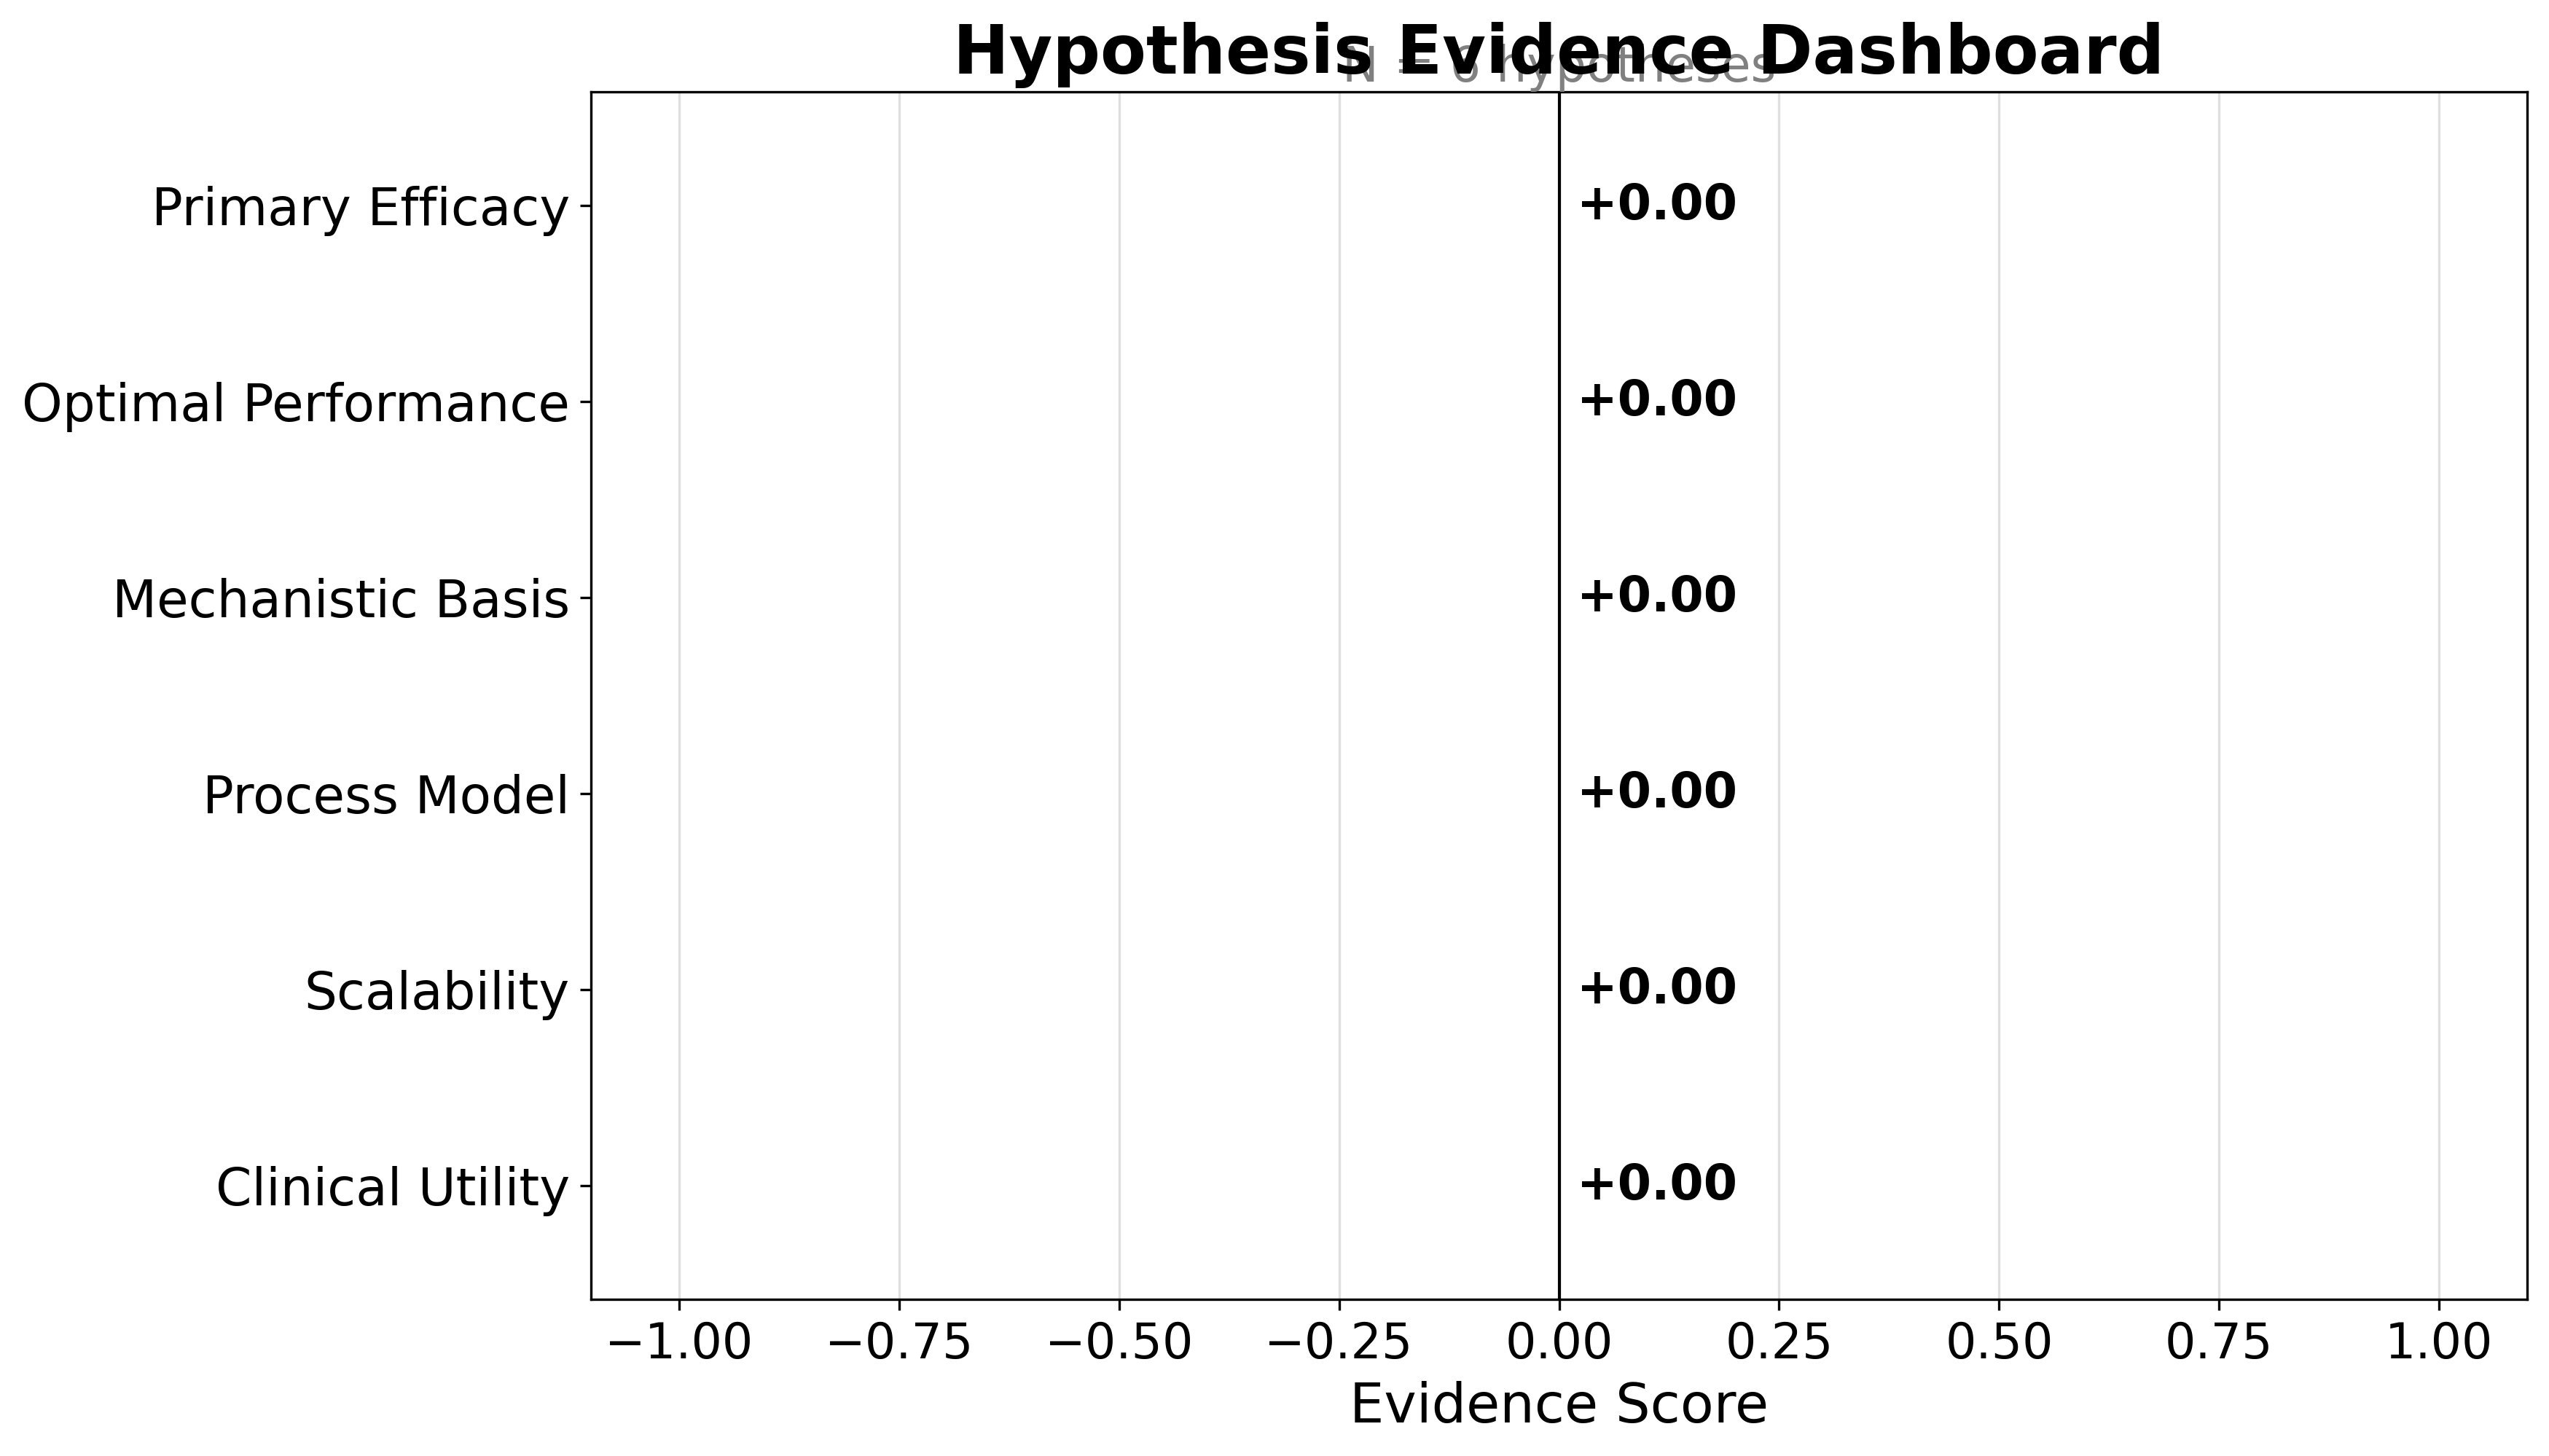
\includegraphics[keepaspectratio,alt={Hypothesis dashboard for Modafinil. The dashboard summarizes the evidence scores across the 6 configured hypotheses, showing the direction and magnitude of citation-weighted assertion evidence.}]{../figures/hypothesis_dashboard.png}}\{\{\#fig:hypothesis\_dashboard\}\}

\newpage

\section{Results: Field Overview}\label{results-field-overview}

The de-duplicated corpus for \textbf{Modafinil} contains \(N = 2302\)
records spanning 2000--2026 (26 years). Publication volume grows at a
compound annual rate of 3.45\% (mean year-over-year growth 6.3\%,
doubling time 11.3 years), peaking in 2025 with 112 records that year.
The growth curve is the first-order signal that the literature is active
rather than dormant.

\pandocbounded{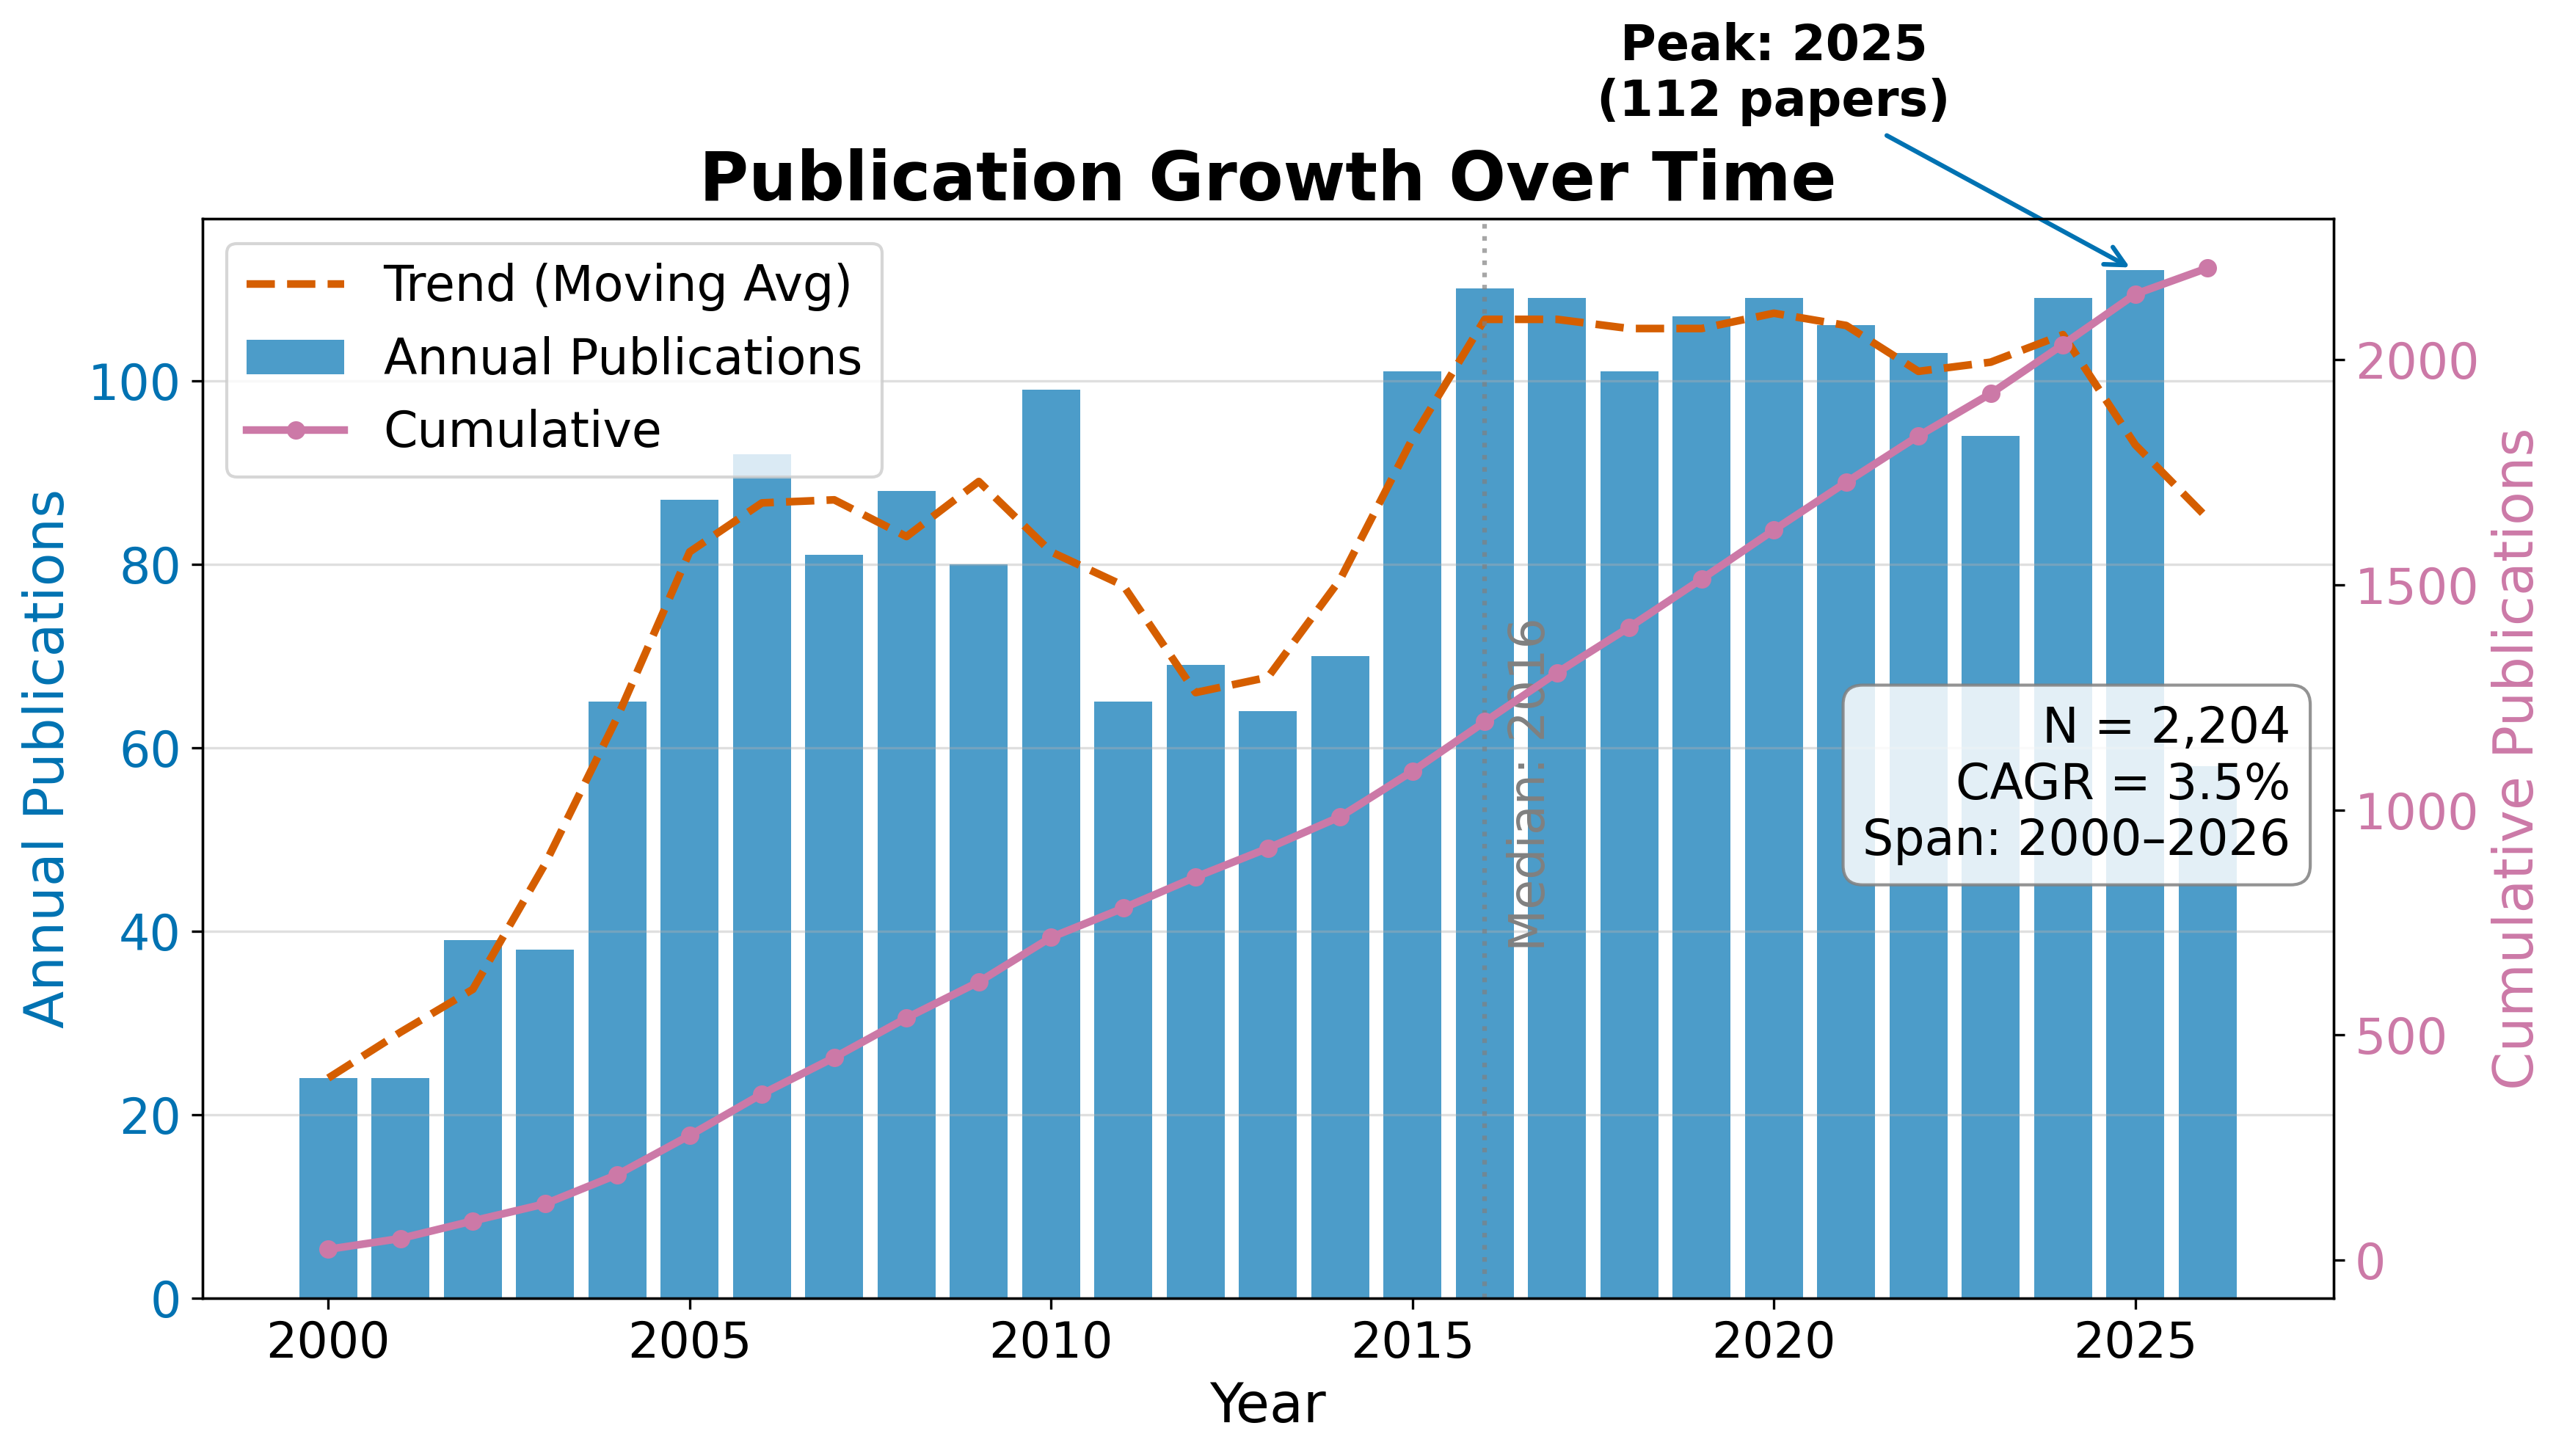
\includegraphics[keepaspectratio,alt={Publication growth curve for Modafinil. Annual publication counts (bars) and cumulative total (line) show sustained growth from 2000 through 2026, peaking in 2025.}]{../figures/growth_curve.png}}\{\{\#fig:growth\_curve\}\}

\subsection{RQ1: Field Size and Growth}\label{rq1-field-size-and-growth}

The temporal analysis reveals a literature that has grown steadily over
26 years. The compound annual growth rate of 3.45\% means the corpus
roughly doubles every 11.3 years --- a pace that exceeds the general
biomedical literature growth rate of approximately 4\% per year. The
peak year 2025 with 112 publications likely reflects both genuine
research activity and the lag between publication and indexing in the
source databases.

\textbf{Table 1. Top publication years.}

{\def\LTcaptype{none} % do not increment counter
\begin{longtable}[]{@{}ll@{}}
\toprule\noalign{}
Year & Publications \\
\midrule\noalign{}
\endhead
\bottomrule\noalign{}
\endlastfoot
2015 & 101 \\
2016 & 110 \\
2017 & 109 \\
2018 & 101 \\
2019 & 107 \\
2020 & 109 \\
2021 & 106 \\
2022 & 103 \\
2024 & 109 \\
2025 & 112 \\
\end{longtable}
}

\subsection{RQ2: Subfield Composition}\label{rq2-subfield-composition}

Records distribute across the 6 configured subfields as shown in Table
2, with \textbf{Clinical Sleep} the largest bucket at 64.3\% of the
classified corpus. The dominance of Clinical Sleep reflects the clinical
primacy of modafinil as a wakefulness-promoting agent: the largest body
of literature addresses its use in narcolepsy, shift-work disorder, and
obstructive sleep apnea.

\textbf{Table 2. Subfield distribution.}

{\def\LTcaptype{none} % do not increment counter
\begin{longtable}[]{@{}lll@{}}
\toprule\noalign{}
Subfield & Papers & Share \\
\midrule\noalign{}
\endhead
\bottomrule\noalign{}
\endlastfoot
Clinical Sleep & 1417 & 64.3\% \\
Cognition & 233 & 10.6\% \\
Pharmacology & 74 & 3.4\% \\
Psychiatry & 357 & 16.2\% \\
Safety & 82 & 3.7\% \\
Neuroscience & 41 & 1.9\% \\
\end{longtable}
}

\pandocbounded{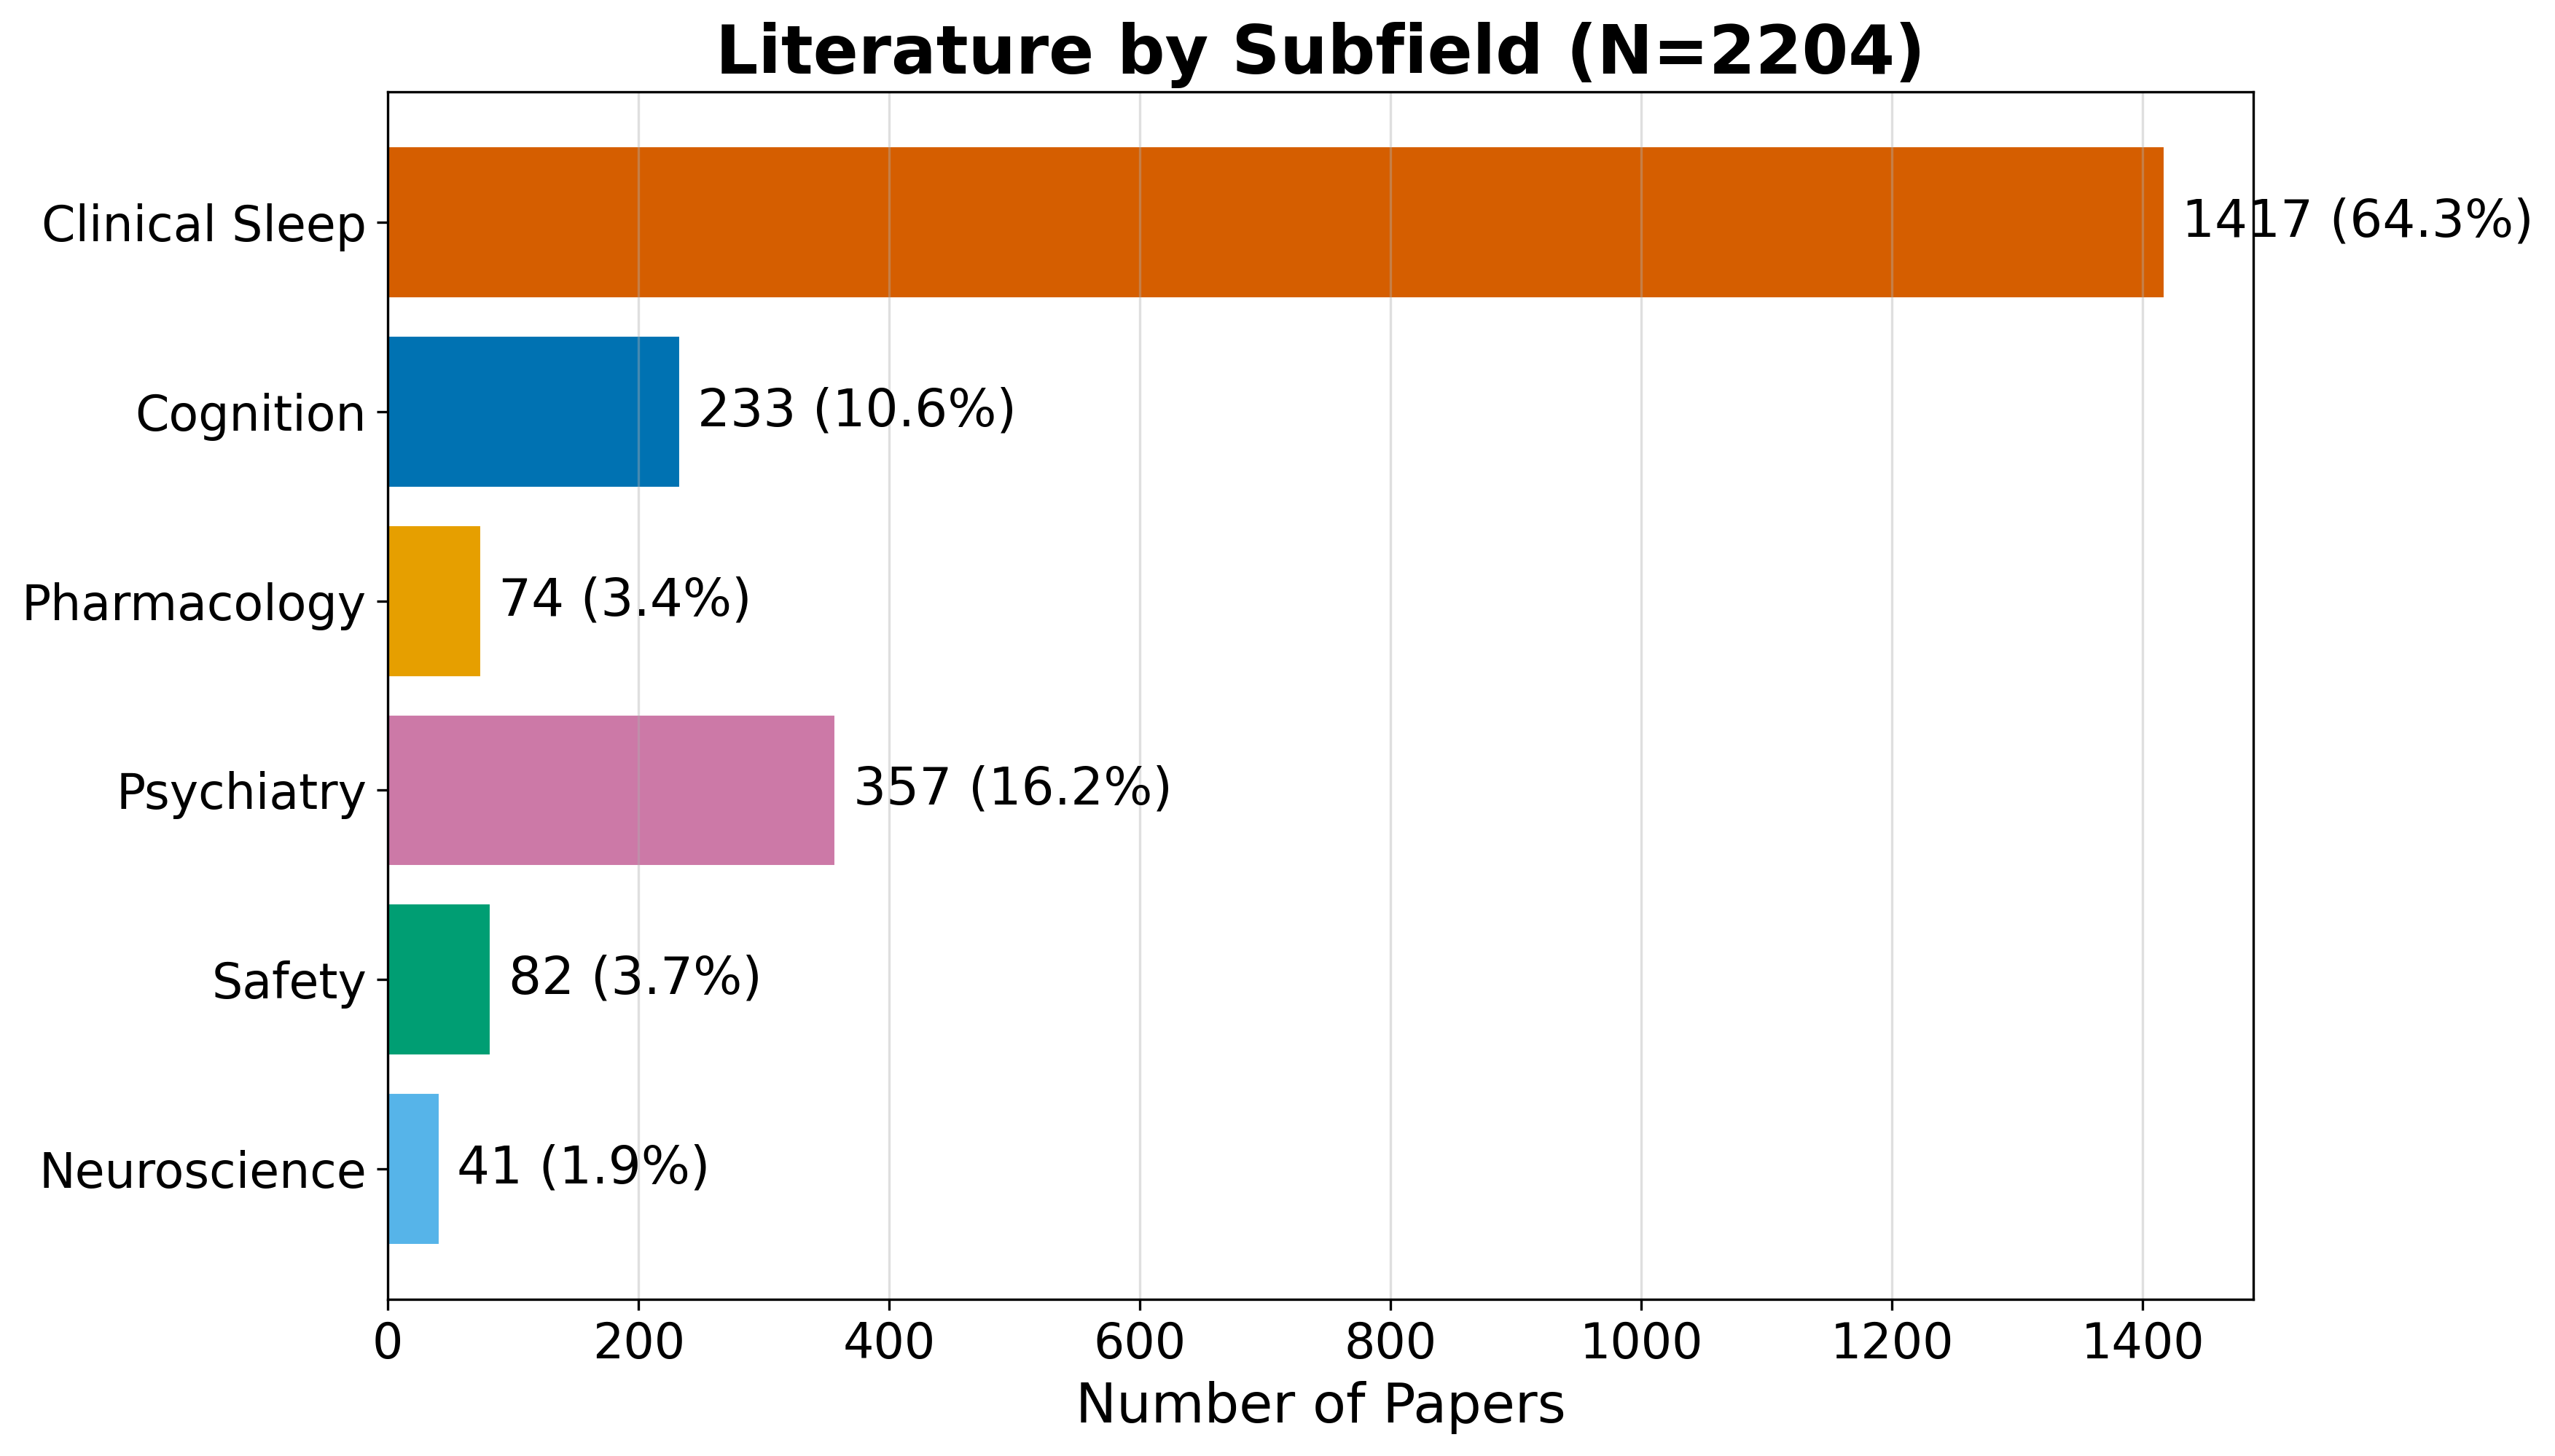
\includegraphics[keepaspectratio,alt={Field summary dashboard for Modafinil. The dashboard combines corpus size, temporal range, subfield distribution, and key bibliometric indicators in a single overview panel.}]{../figures/field_summary.png}}\{\{\#fig:field\_summary\}\}

\pandocbounded{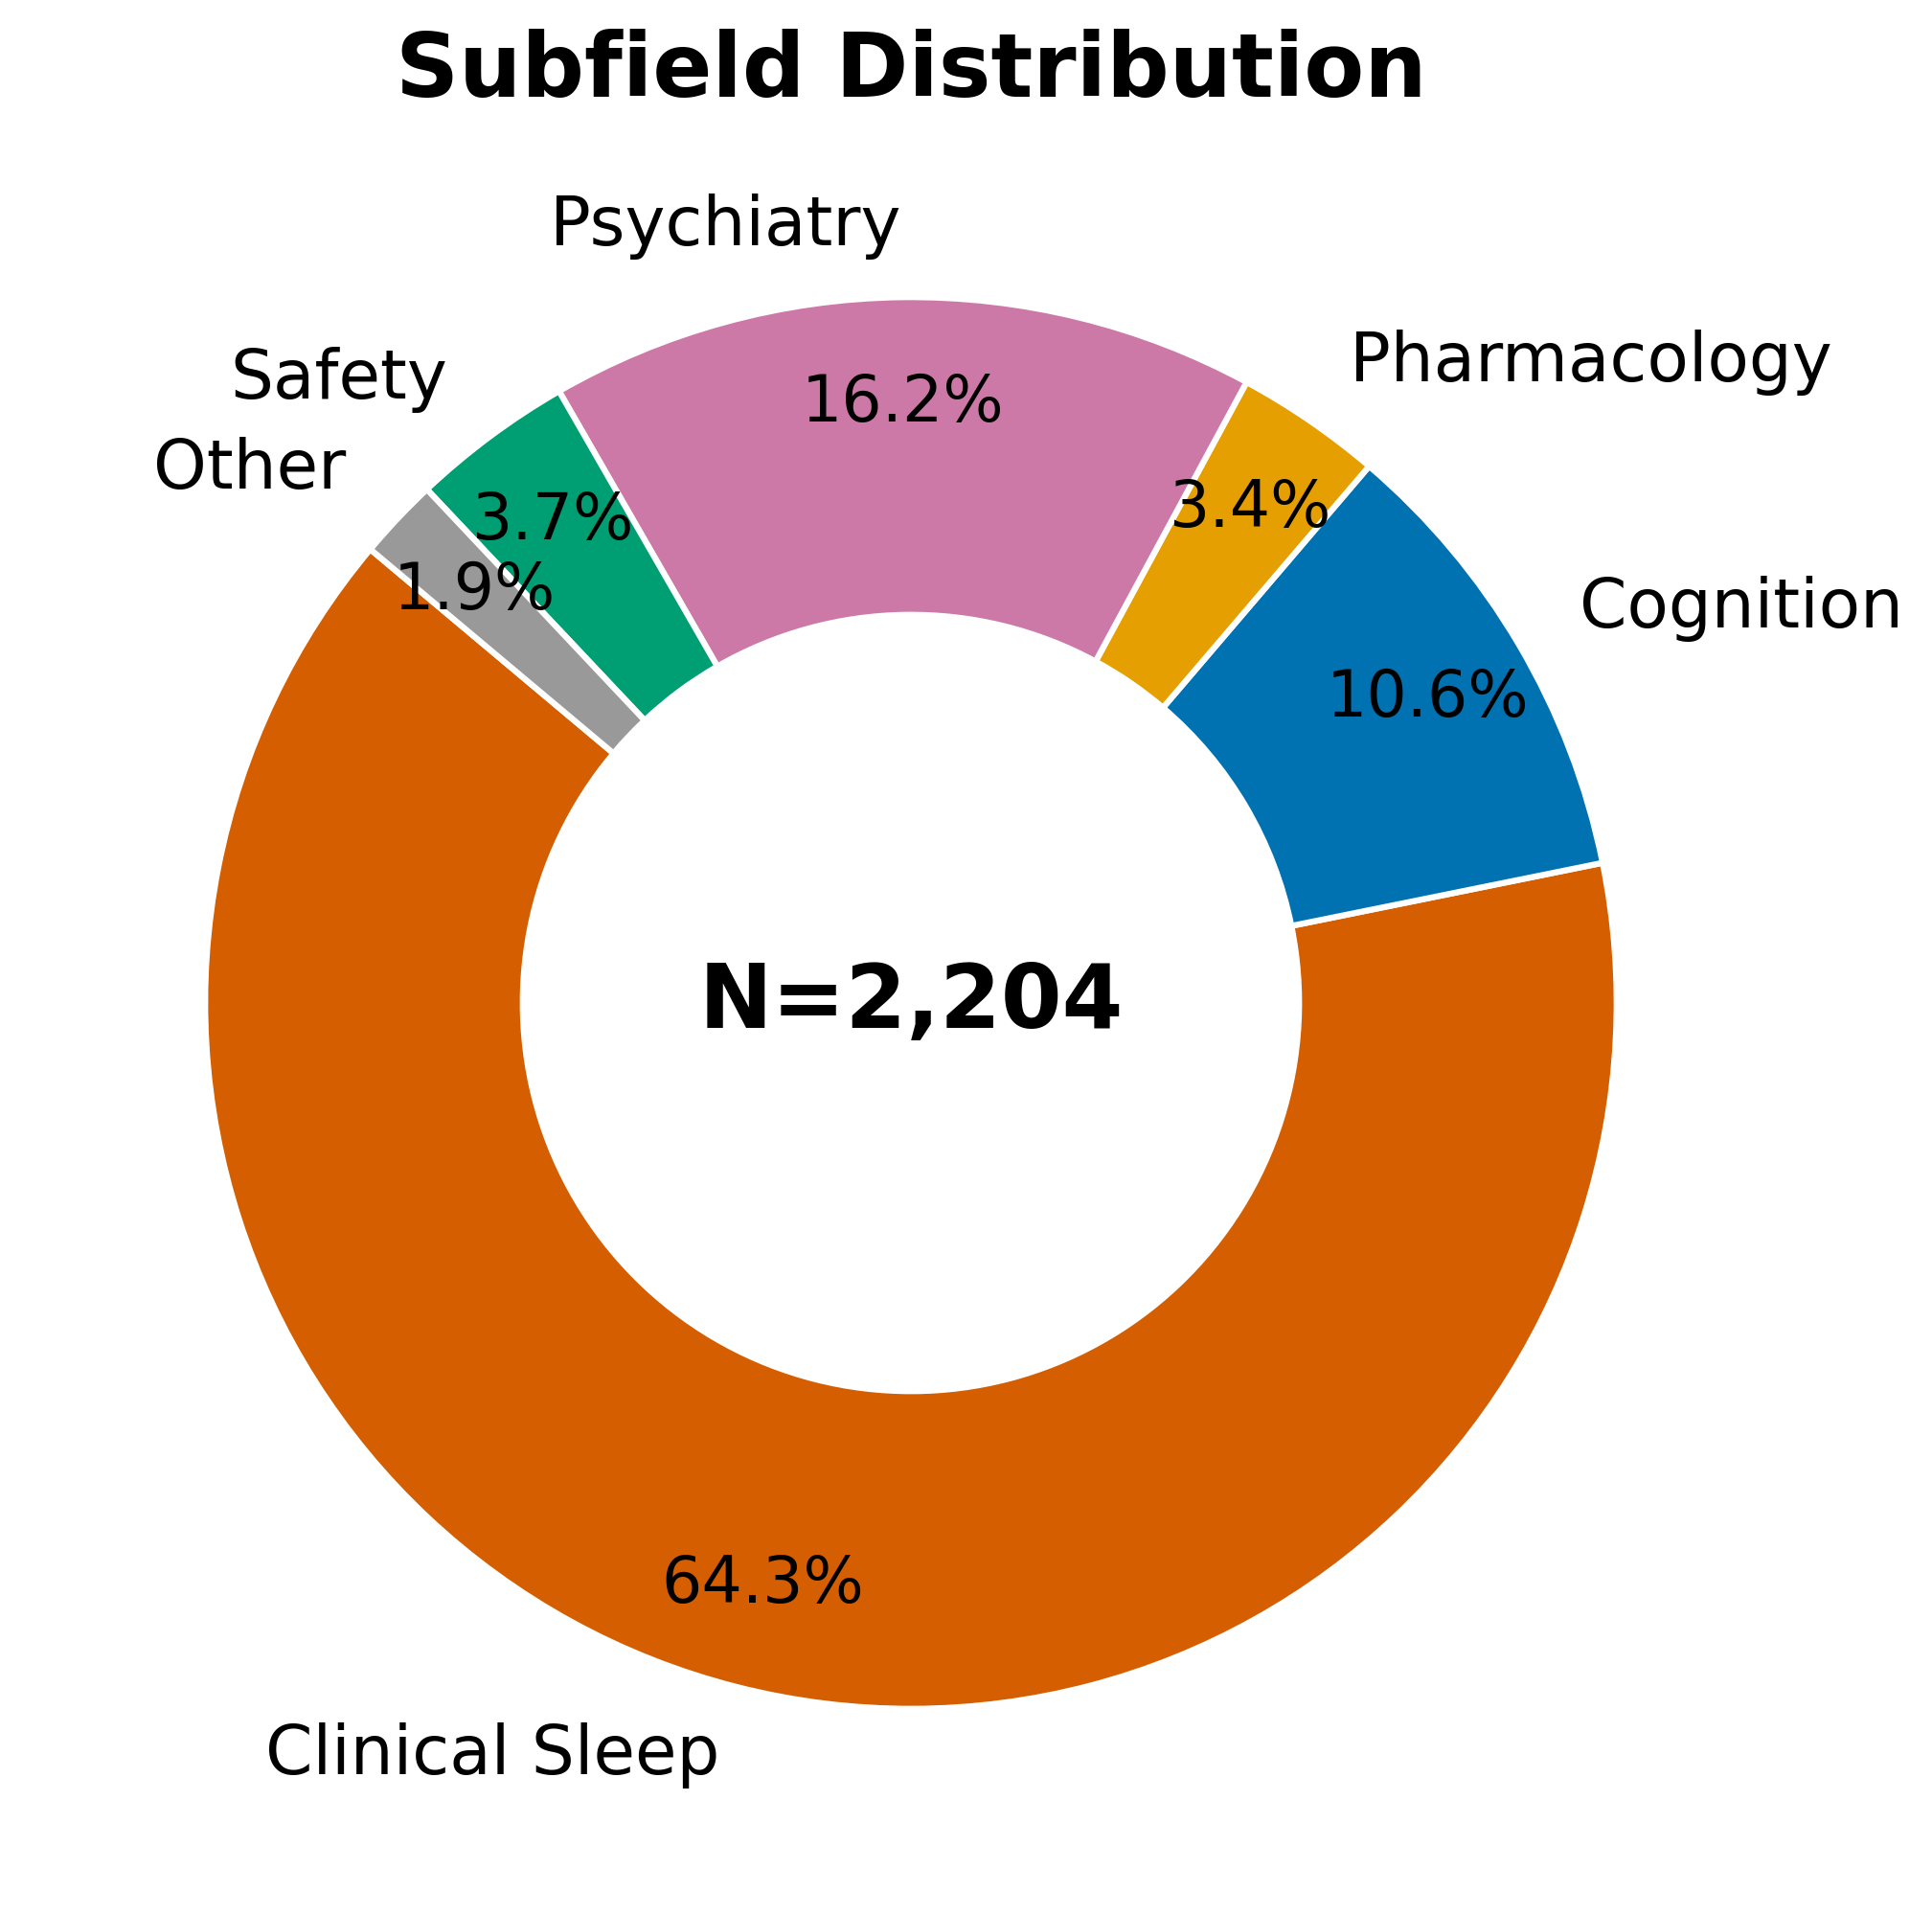
\includegraphics[keepaspectratio,alt={Subfield distribution for Modafinil. The 6-bucket taxonomy shows the relative weight of each configured sub-area, with Clinical Sleep dominant at 64.3\%.}]{../figures/subfield_distribution.png}}\{\{\#fig:subfield\_distribution\}\}

\pandocbounded{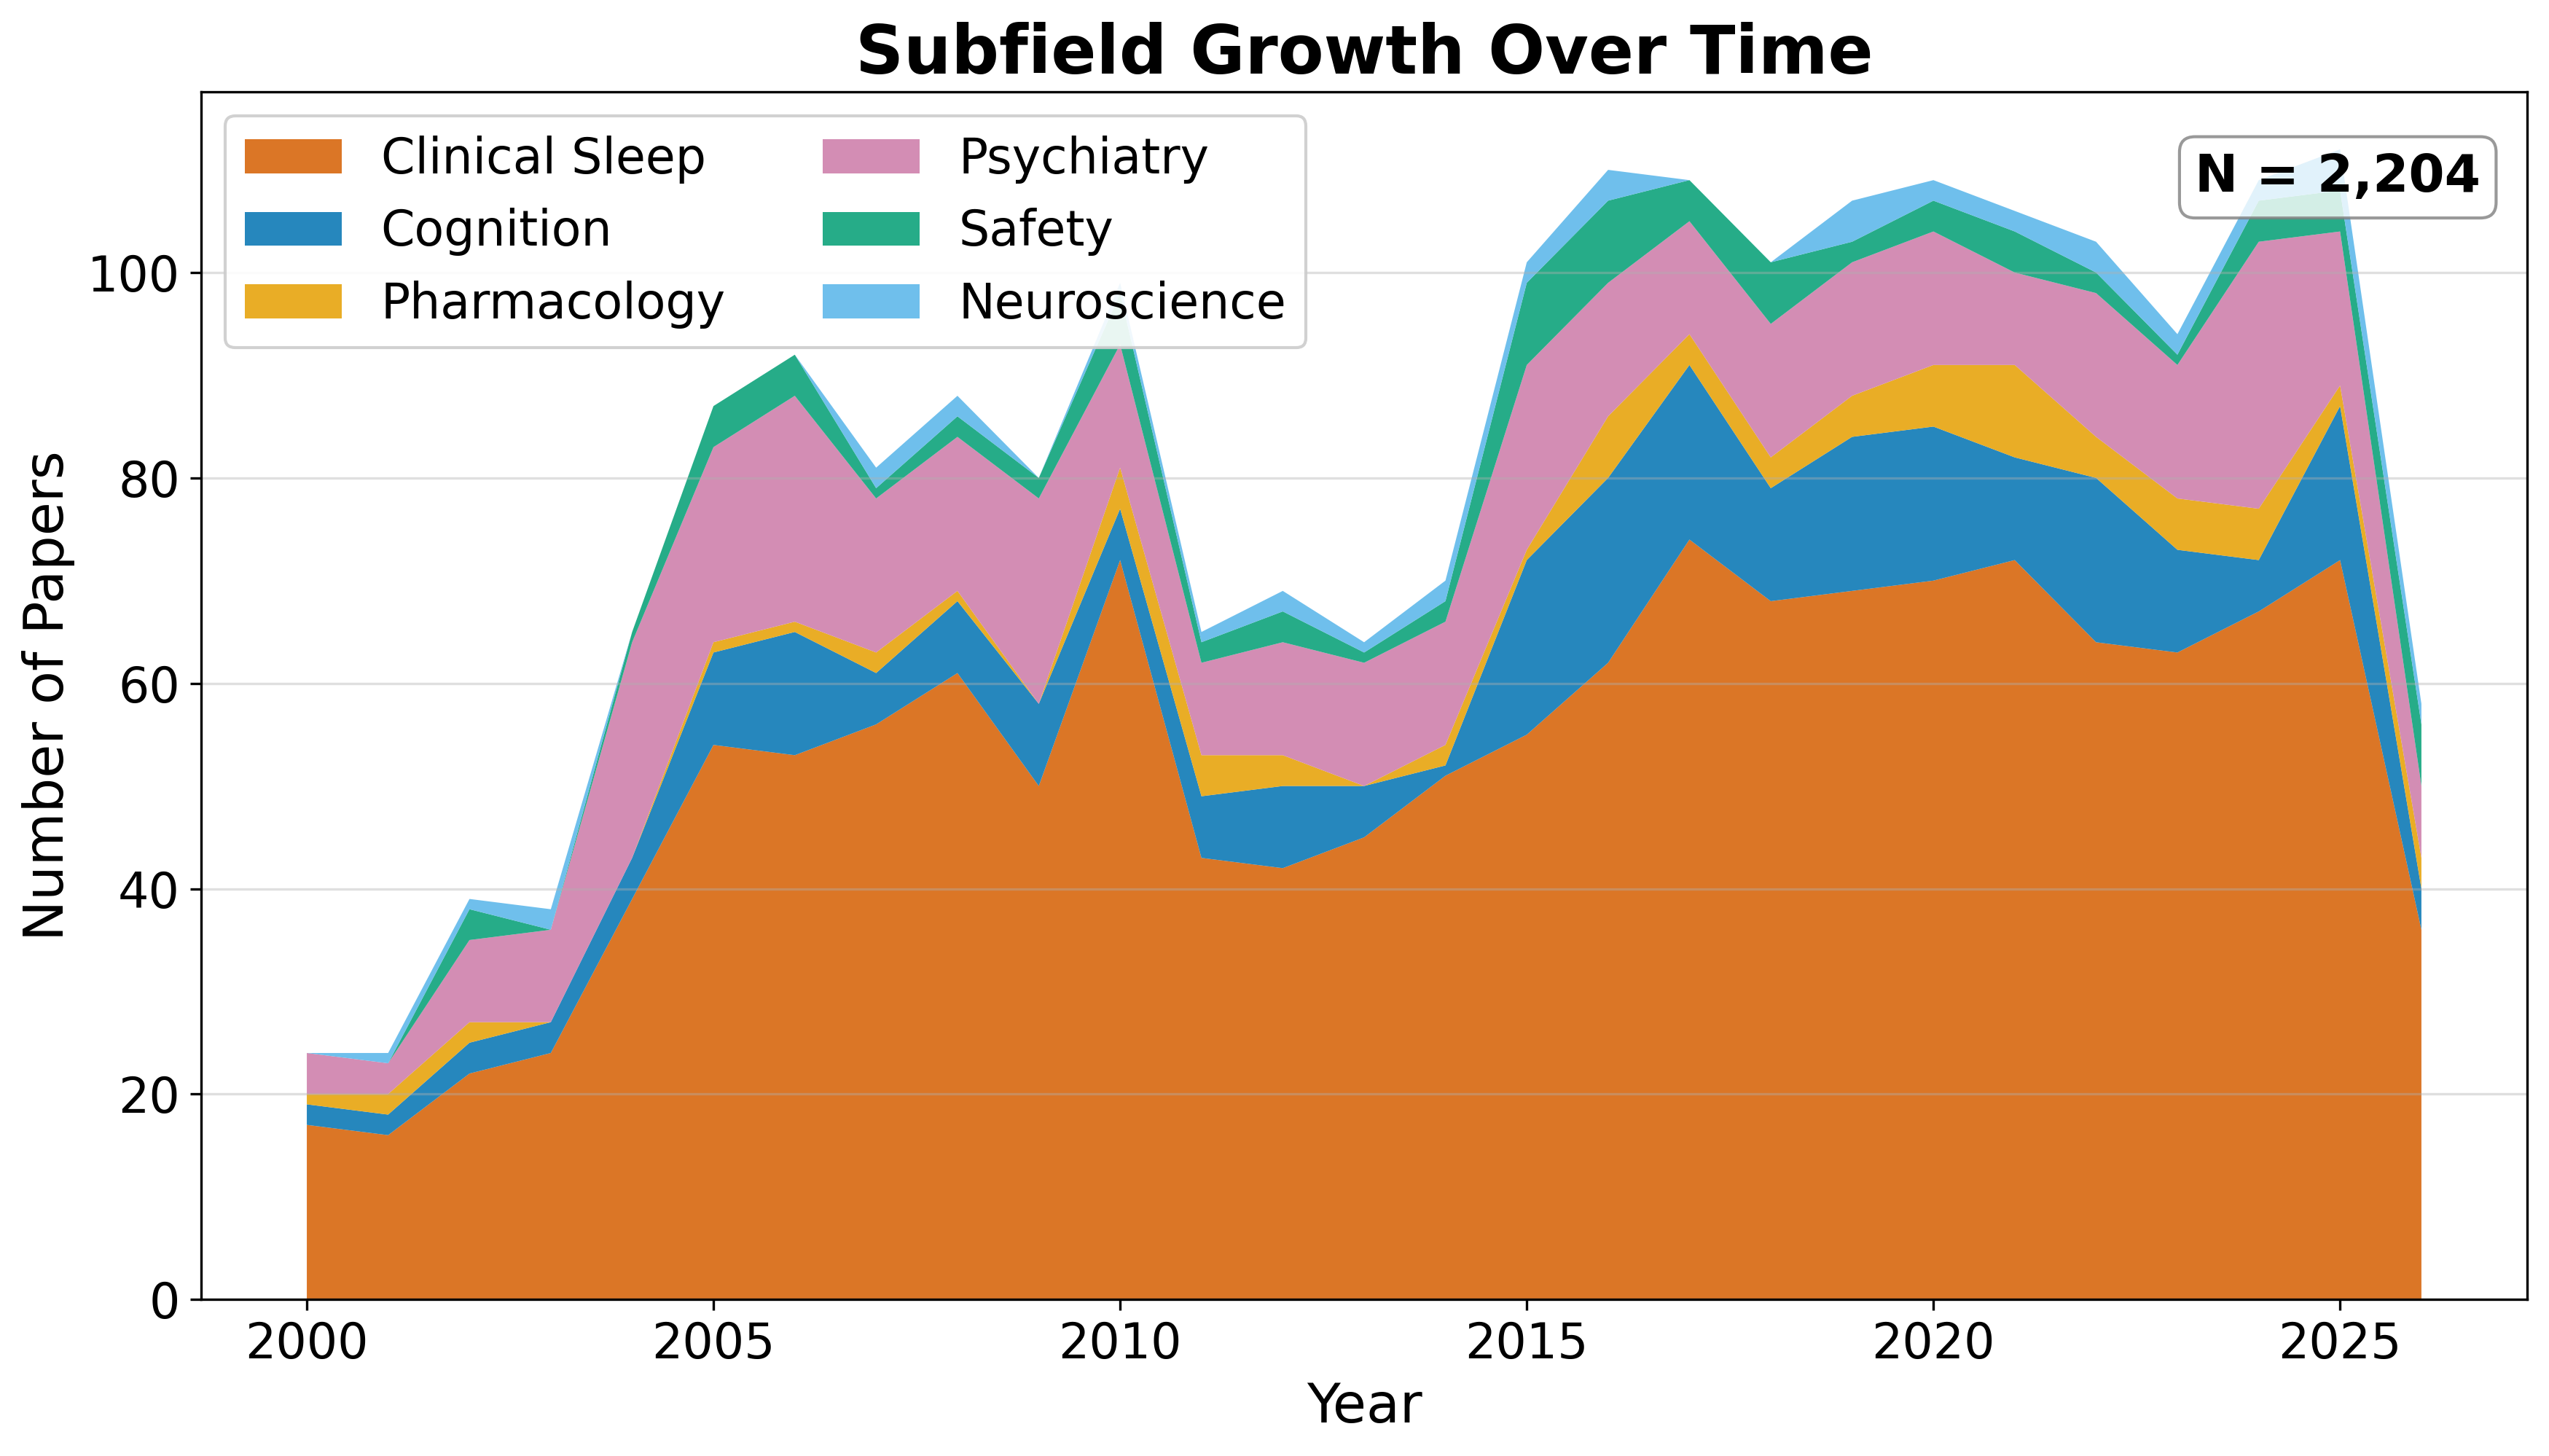
\includegraphics[keepaspectratio,alt={Subfield timeline for Modafinil. Stacked annual publication counts by subfield show how each sub-area has evolved over time, revealing emerging and declining research threads.}]{../figures/subfield_timeline.png}}\{\{\#fig:subfield\_timeline\}\}

\subsection{Identifier and Full-Text
Coverage}\label{identifier-and-full-text-coverage}

The corpus has strong identifier coverage: 2248 of 2302 records (98.0\%)
carry DOIs, enabling robust cross-engine de-duplication. OpenAlex IDs
are present for 932 records. Abstract coverage stands at 55.5\% (1277
records), which limits the text analytics to that subset. Open-access
status is confirmed for 14.4\% of records, and 40.9\% have a direct PDF
link.

\subsection{Descriptive Bibliometrics}\label{descriptive-bibliometrics}

The corpus spans 7259 unique authors across 2302 papers, yielding a mean
of 1.34 papers per author. Citation counts range from zero to 1333 (mean
30.9, median 0.0), with a total of 68,151 citations across the corpus.
The Gini coefficient of citation concentration is 0.812, indicating a
highly skewed distribution characteristic of scientific literature.

\textbf{Table 3. Citation count distribution.}

{\def\LTcaptype{none} % do not increment counter
\begin{longtable}[]{@{}ll@{}}
\toprule\noalign{}
Citations & Papers \\
\midrule\noalign{}
\endhead
\bottomrule\noalign{}
\endlastfoot
0 & 1184 \\
1-9 & 195 \\
10-49 & 421 \\
50-99 & 214 \\
100-499 & 179 \\
500+ & 11 \\
\end{longtable}
}

\pandocbounded{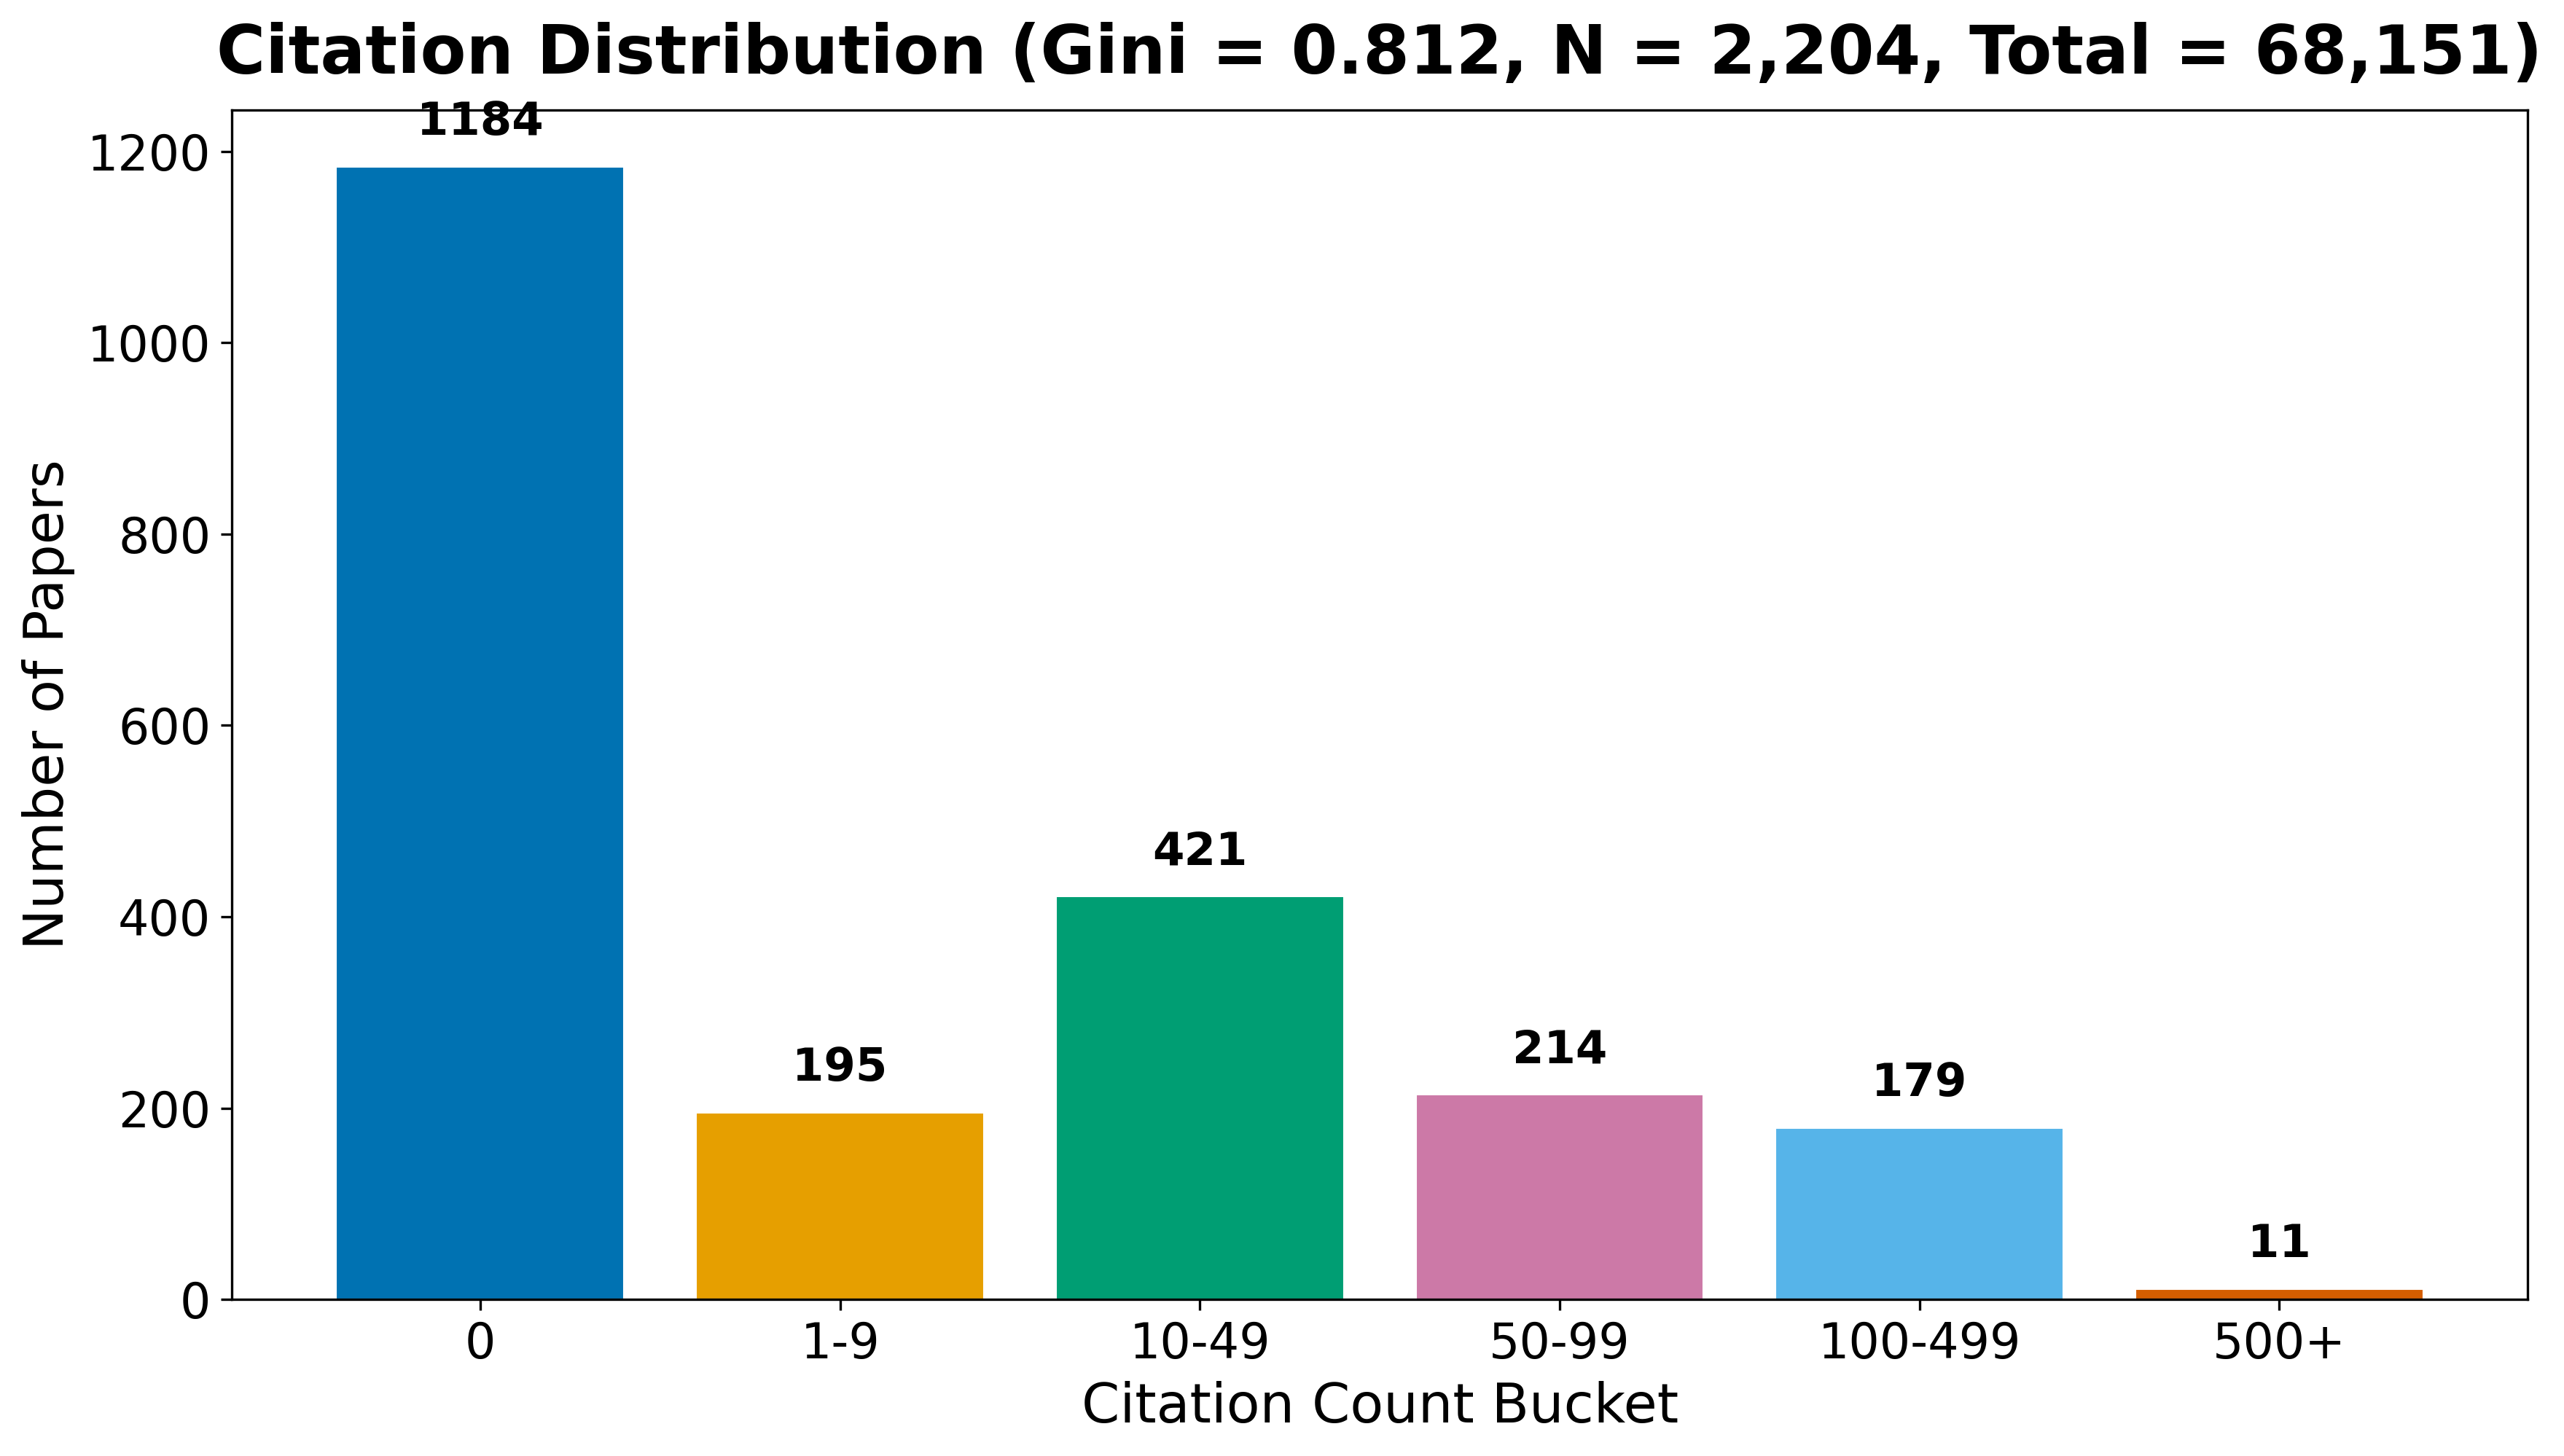
\includegraphics[keepaspectratio,alt={Citation distribution for Modafinil. The histogram shows the number of papers in each citation-count bucket, with the Gini coefficient annotated. The heavy-tailed distribution is characteristic of scientific citation networks.}]{../figures/citation_distribution.png}}\{\{\#fig:citation\_distribution\}\}

\textbf{Table 4. Top publication venues.}

{\def\LTcaptype{none} % do not increment counter
\begin{longtable}[]{@{}ll@{}}
\toprule\noalign{}
Venue & Papers \\
\midrule\noalign{}
\endhead
\bottomrule\noalign{}
\endlastfoot
Reactions Weekly & 142 \\
Psychopharmacology & 41 \\
SLEEP & 34 \\
Sleep Medicine & 33 \\
The Journal of Clinical Psychiatry & 31 \\
European Neuropsychopharmacology & 27 \\
Neuropharmacology & 26 \\
Inpharma Weekly & 25 \\
PubMed & 24 \\
American Journal of Psychiatry & 23 \\
\end{longtable}
}

\pandocbounded{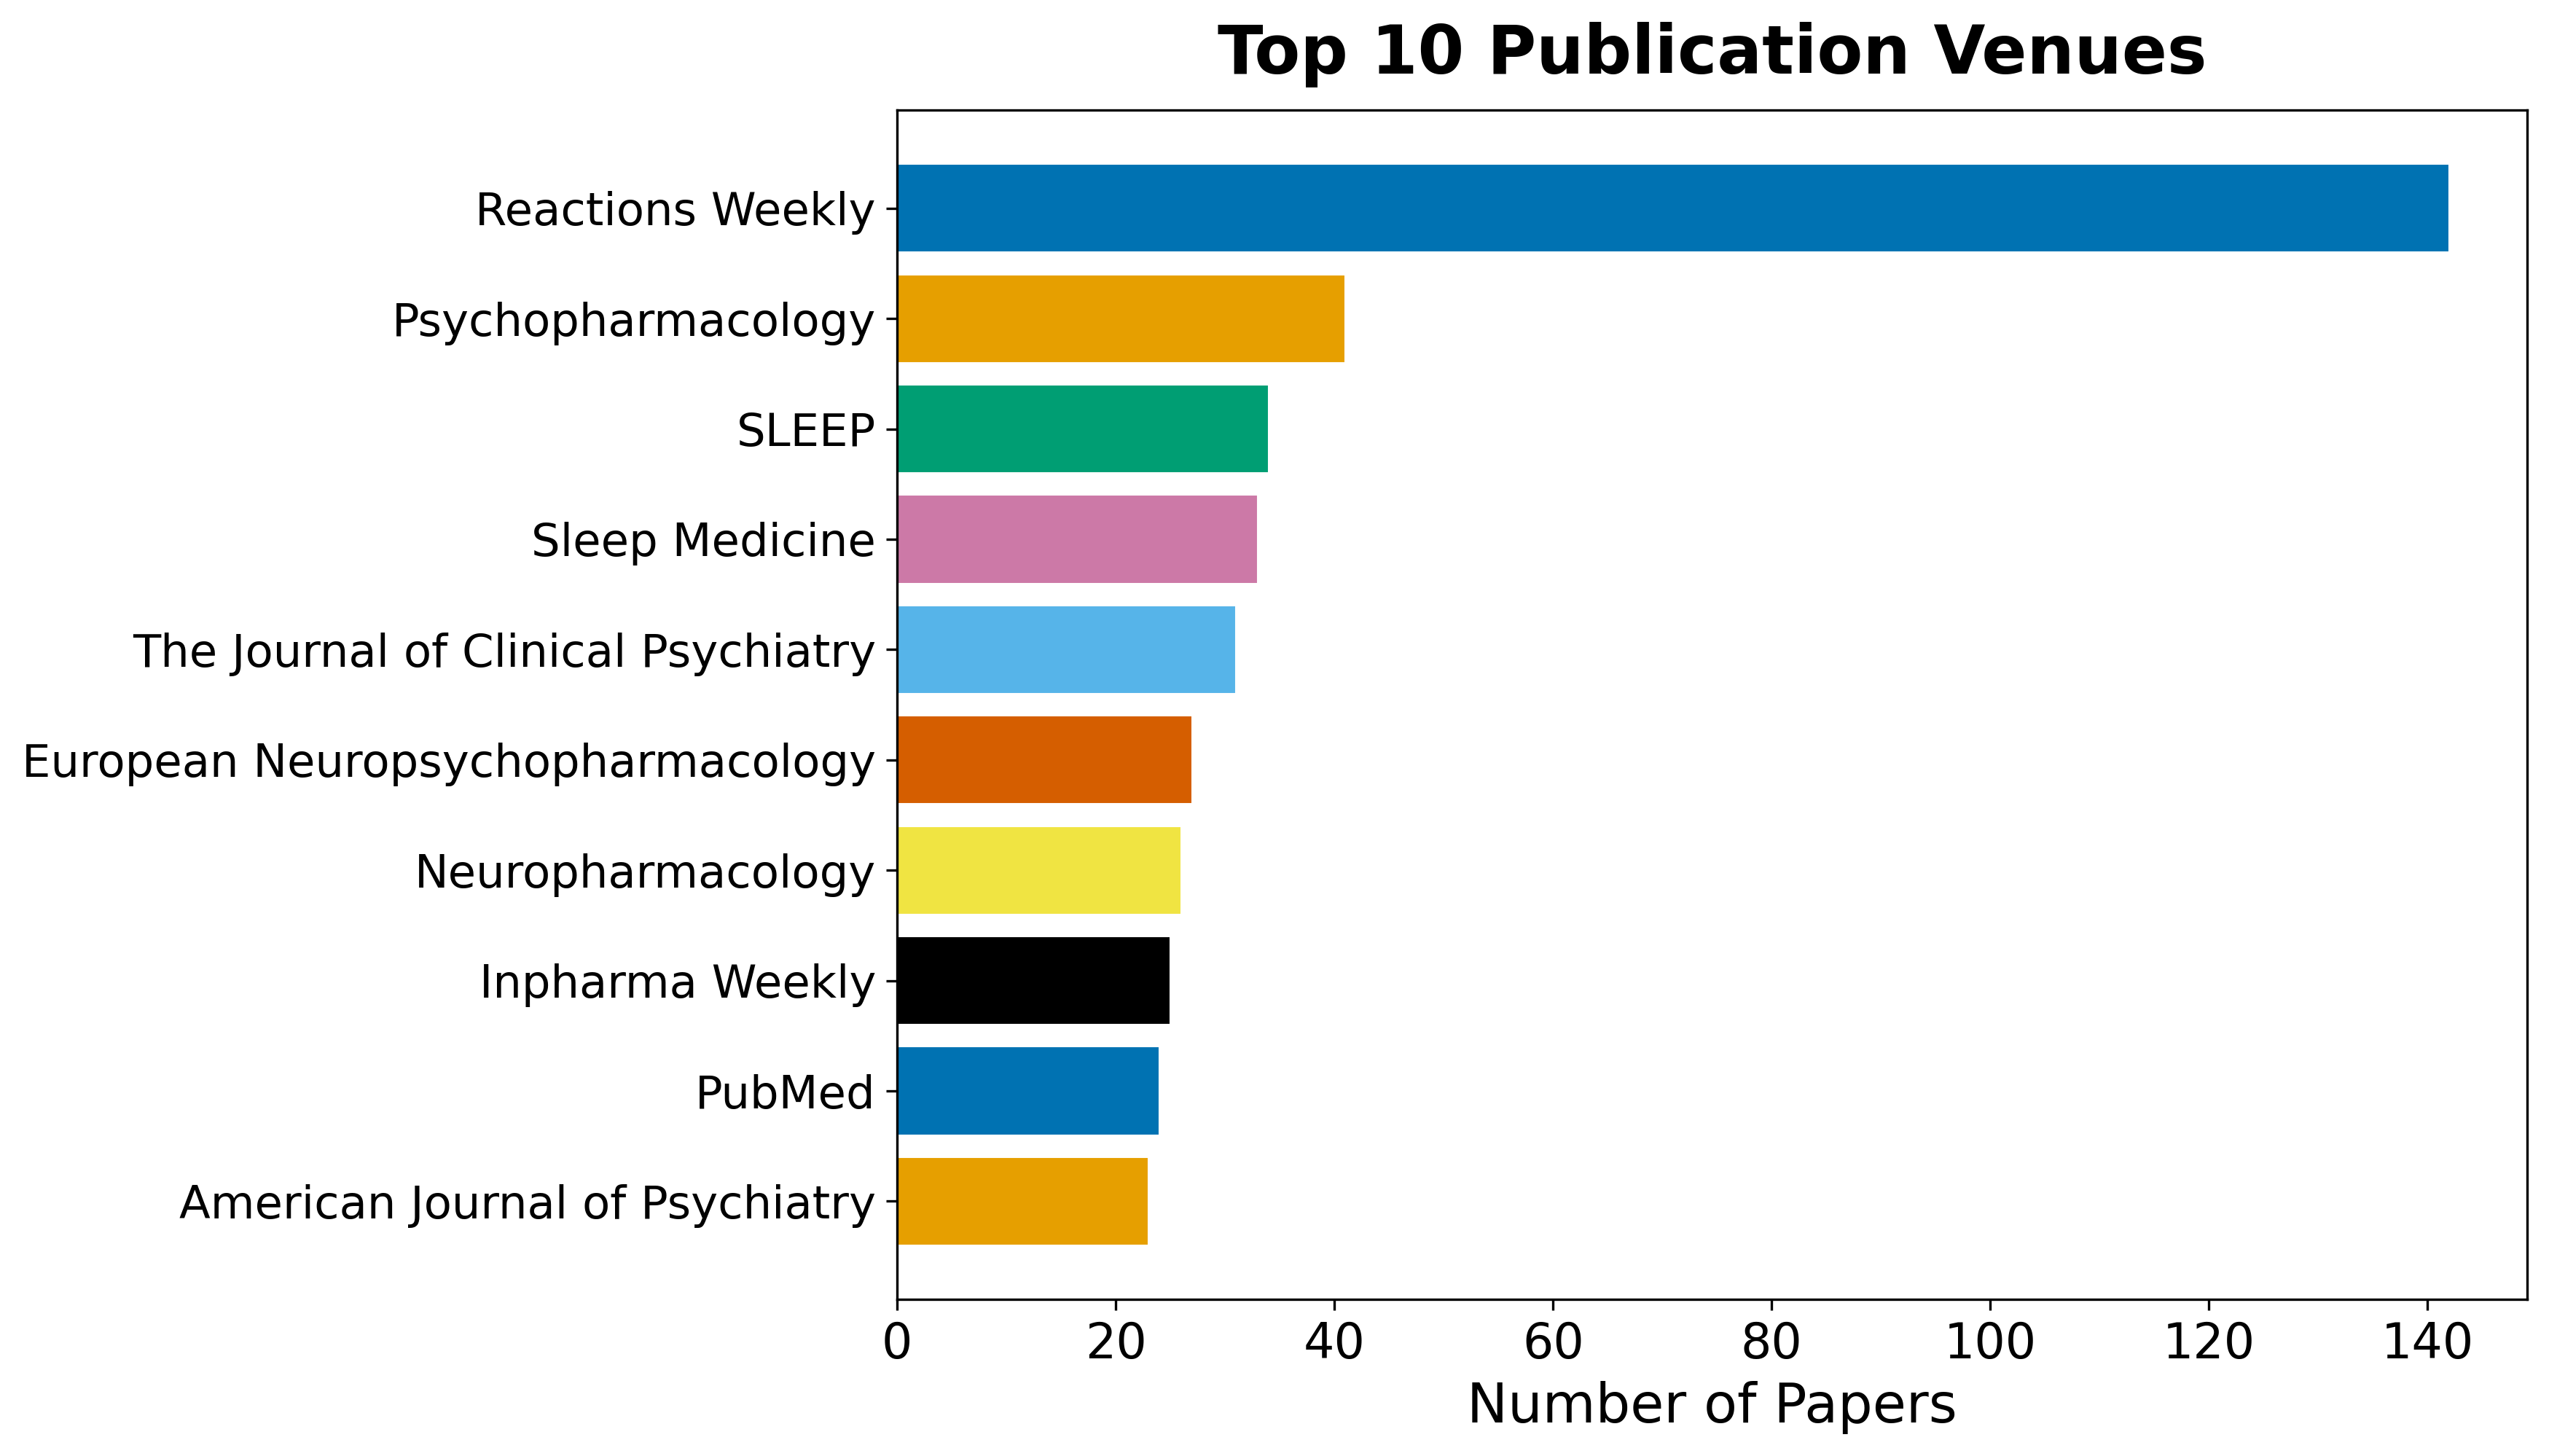
\includegraphics[keepaspectratio,alt={Top publication venues for Modafinil. The horizontal bar chart shows the 15 venues with the most papers in the corpus, revealing where the modafinil literature is published.}]{../figures/top_venues.png}}\{\{\#fig:top\_venues\}\}

\textbf{Table 5. Top authors by publication count.}

{\def\LTcaptype{none} % do not increment counter
\begin{longtable}[]{@{}lll@{}}
\toprule\noalign{}
Rank & Author & Papers \\
\midrule\noalign{}
\endhead
\bottomrule\noalign{}
\endlastfoot
1 & \&NA; & 66 \\
2 & Ronghua Yang & 26 \\
3 & Yves Dauvilliers & 26 \\
4 & Amy Hauck Newman & 22 \\
5 & Barbara J. Sahakian & 20 \\
6 & Edward T. Hellriegel & 17 \\
7 & Gianluigi Tanda & 16 \\
8 & Philmore Robertson & 16 \\
9 & Sanjay Arora & 16 \\
10 & Gert Lubec & 15 \\
\end{longtable}
}

\pandocbounded{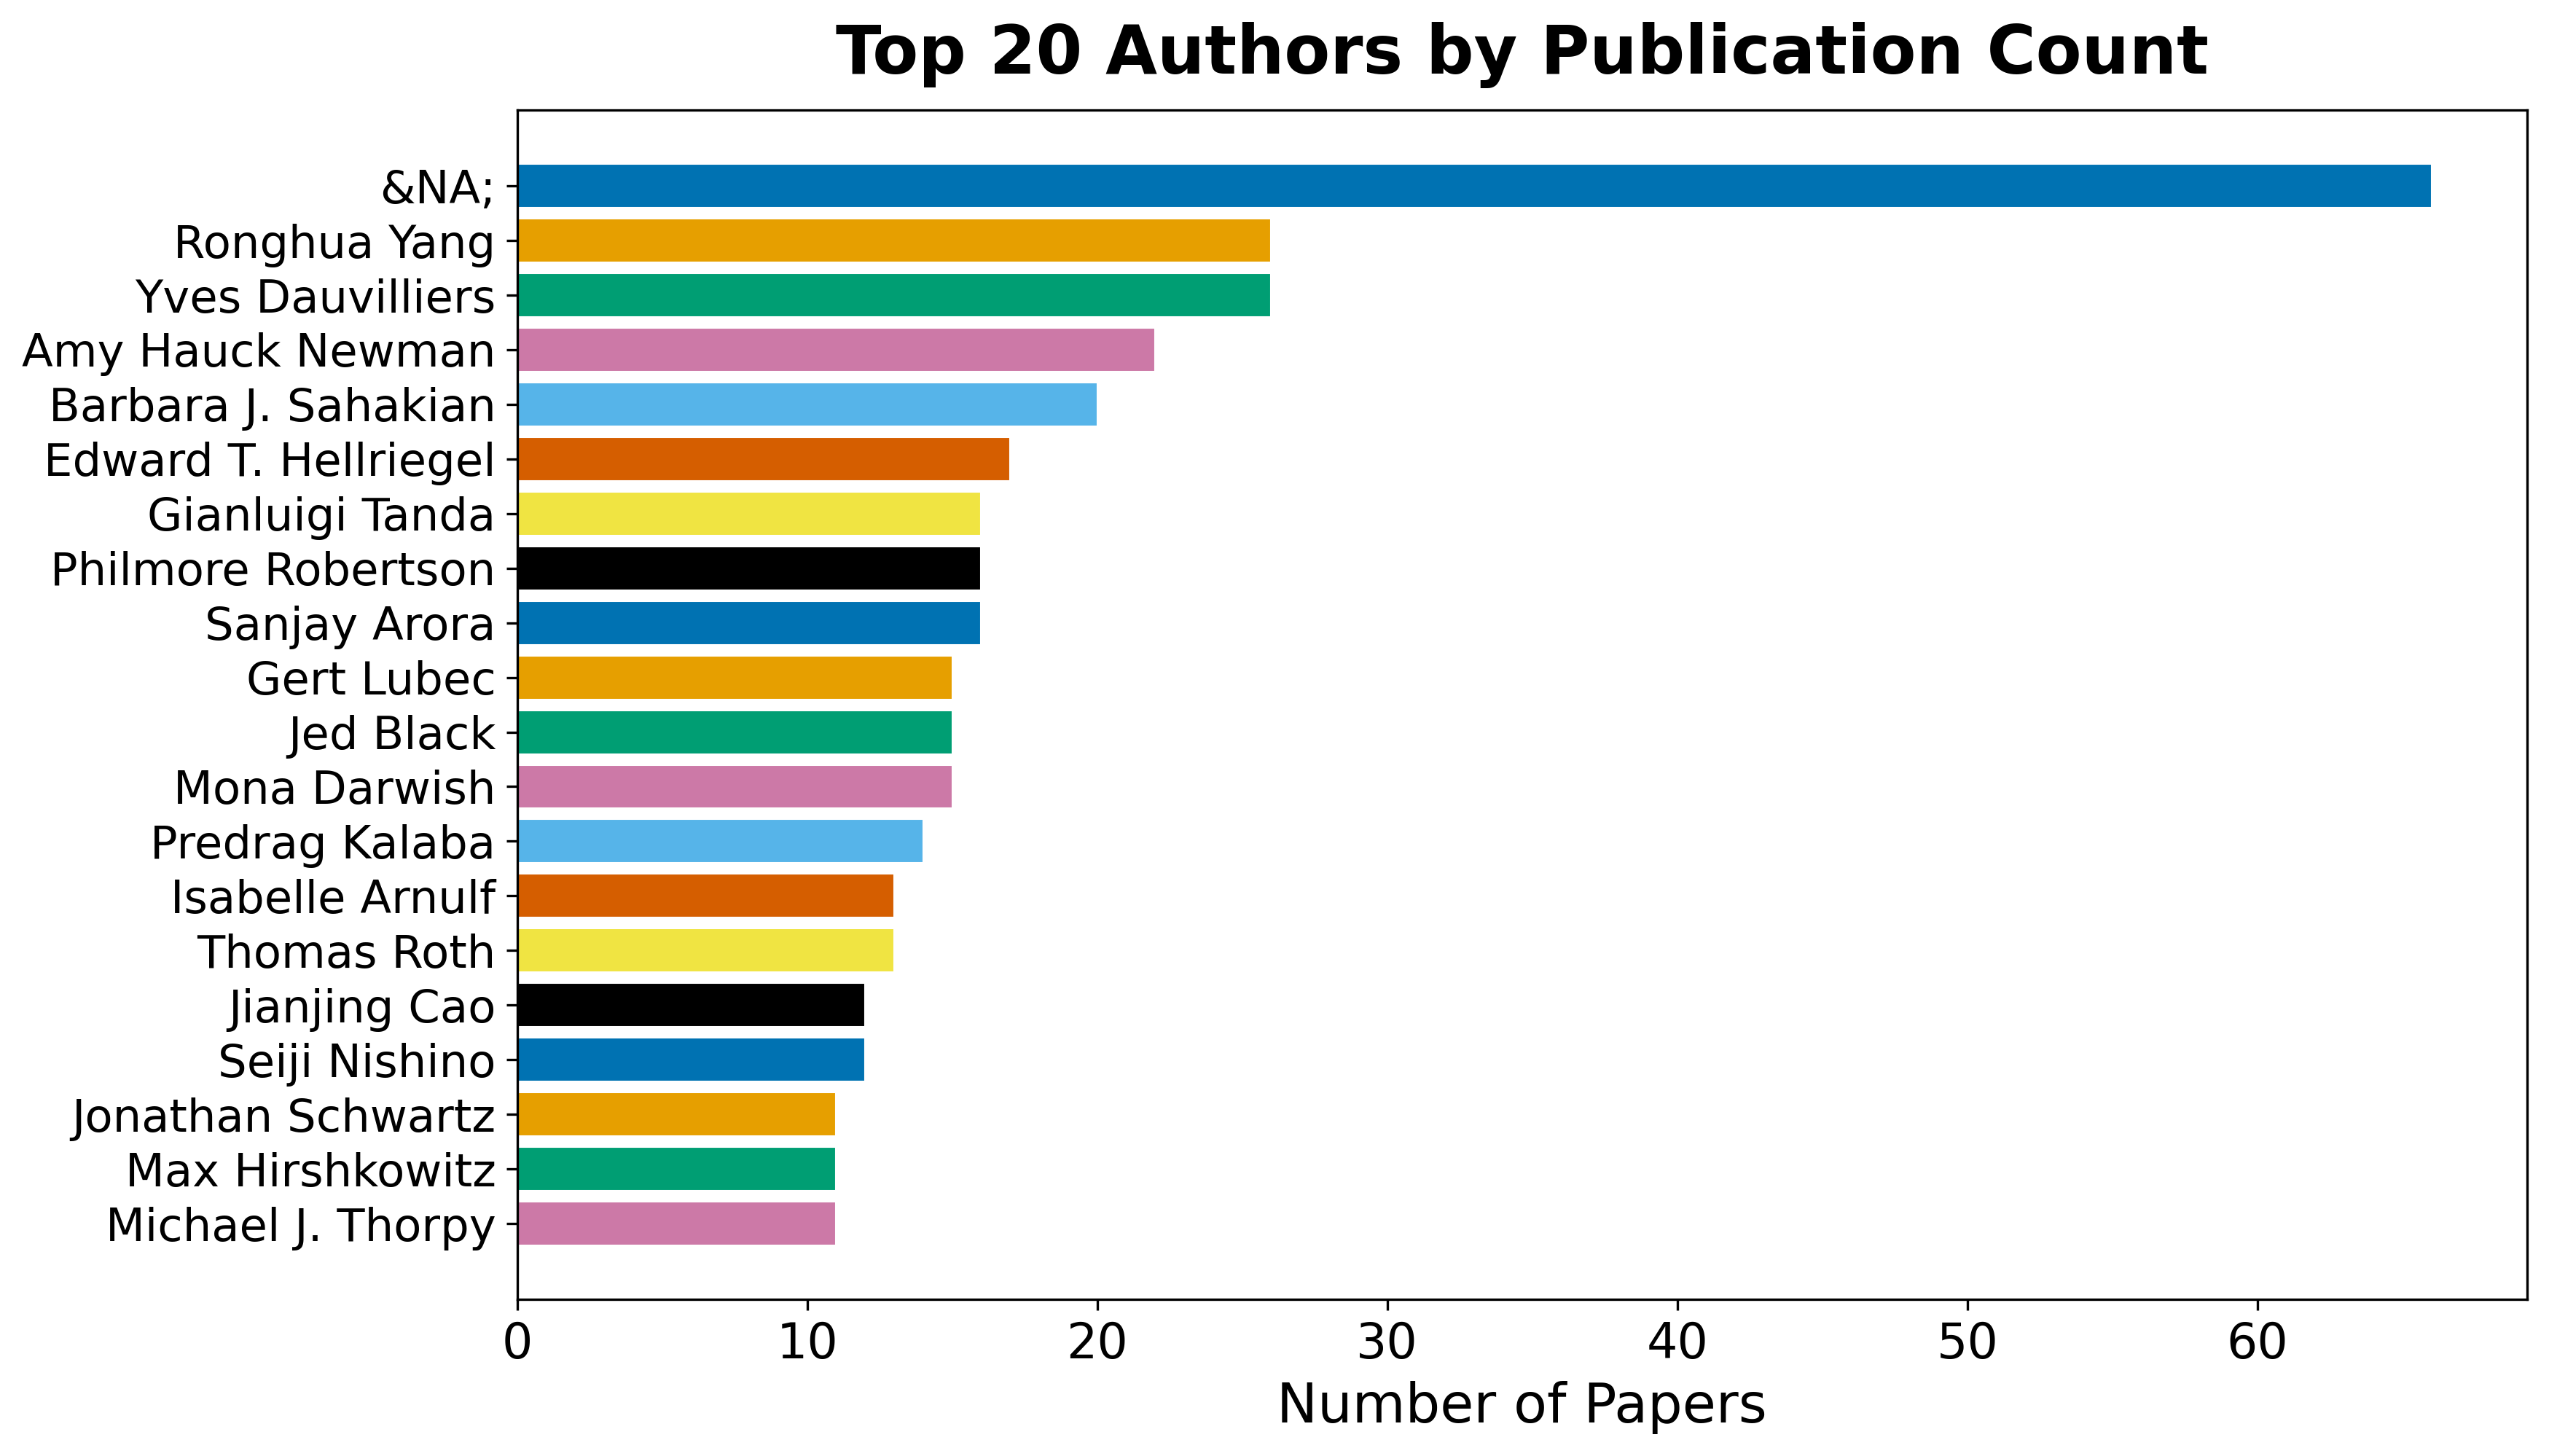
\includegraphics[keepaspectratio,alt={Author productivity for Modafinil. The horizontal bar chart shows the 20 authors with the most papers in the corpus, revealing the most prolific contributors to the modafinil literature.}]{../figures/author_productivity.png}}\{\{\#fig:author\_productivity\}\}

\newpage

\section{Results: Subfield Structure}\label{results-subfield-structure}

The subfield taxonomy is defined entirely in configuration; for this
instance it spans 6 buckets (Clinical Sleep, Cognition, Pharmacology,
Psychiatry, Safety, and Neuroscience). Each record is assigned to the
highest-priority bucket whose keywords it matches, so the distribution
reflects the configured taxonomy rather than a fixed schema. Table 2
(previous section) reports the counts; the largest bucket is
\textbf{Clinical Sleep} (64.3\%).

\subsection{Per-Subfield
Characterization}\label{per-subfield-characterization}

The subfield breakdown reveals the multi-disciplinary nature of the
modafinil literature:

\begin{itemize}
\item
  \textbf{Clinical Sleep} dominates at 64.3\%, reflecting the drug's
  primary indication for narcolepsy, shift-work disorder, and
  obstructive sleep apnea. This bucket includes randomized controlled
  trials, meta-analyses of efficacy, and long-term safety studies in
  sleep-disorder populations.
\item
  \textbf{Cognition} represents studies of cognitive enhancement,
  working memory, attention, and executive function --- particularly in
  sleep-deprived populations. This subfield has grown with the broader
  interest in neuroenhancement and ``smart drugs.''
\item
  \textbf{Pharmacology} covers pharmacokinetics, mechanism of action
  (dopamine transporter inhibition, orexin system interactions),
  metabolism, and drug interactions.
\item
  \textbf{Psychiatry} addresses off-label uses including ADHD,
  depression, bipolar disorder, and schizophrenia --- often as an
  adjunctive therapy targeting fatigue and cognitive symptoms.
\item
  \textbf{Safety} encompasses adverse effects, abuse potential,
  dependence, tolerability, and rare but serious events such as
  Stevens-Johnson syndrome.
\item
  \textbf{Neuroscience} includes neuroimaging (fMRI, EEG),
  orexin/hypothalamus studies, and preclinical mechanistic work.
\end{itemize}

Because the taxonomy is data, not code, re-targeting the template to
another topic --- or refining the buckets for the same topic --- changes
this section's structure and numbers without any change to the analysis
code. The subfield assignment also feeds the temporal and citation
analyses, allowing per-subfield growth and connectivity to be read off
the same artifacts.

\newpage

\section{Results: Language, Topics, and
Embeddings}\label{results-language-topics-and-embeddings}

\subsection{RQ3: Topical and Linguistic
Structure}\label{rq3-topical-and-linguistic-structure}

Text analysis operates over titles, abstracts, and (when available) full
text. A TF-IDF representation over a 500-feature vocabulary feeds
non-negative matrix factorization, which extracts 5 latent topics
cross-cutting the subfield taxonomy. The top vocabulary terms are:
modafinil, treatment, study, effects, patients, results, sleep, used,
use, drug, studies, clinical, mg, using, placebo, cognitive, associated,
effect, however, disorder.

\textbf{Table 3. NMF topics extracted from the corpus.}

{\def\LTcaptype{none} % do not increment counter
\begin{longtable}[]{@{}
  >{\raggedright\arraybackslash}p{(\linewidth - 2\tabcolsep) * \real{0.5000}}
  >{\raggedright\arraybackslash}p{(\linewidth - 2\tabcolsep) * \real{0.5000}}@{}}
\toprule\noalign{}
\begin{minipage}[b]{\linewidth}\raggedright
Topic
\end{minipage} & \begin{minipage}[b]{\linewidth}\raggedright
Top terms
\end{minipage} \\
\midrule\noalign{}
\endhead
\bottomrule\noalign{}
\endlastfoot
0 & cognitive, use, drugs, enhancement, performance, drug, effects,
modafinil \\
1 & adhd, ci, 95, studies, trials, evidence, risk, treatment \\
2 & modafinil, mg, kg, effects, dose, rats, induced, placebo \\
3 & sleep, narcolepsy, sleepiness, patients, eds, daytime, excessive,
cataplexy \\
4 & fatigue, patients, placebo, modafinil, scale, depression, treatment,
armodafinil \\
\end{longtable}
}

The topics reveal the thematic structure of the literature: Topic 0
centres on cognitive enhancement and neuroenhancement; Topic 1 addresses
ADHD treatment and clinical evidence; Topic 2 covers pharmacological
dose-response studies (including animal models); Topic 3 focuses on
sleep disorders (narcolepsy, excessive daytime sleepiness); and Topic 4
addresses fatigue in psychiatric populations. These topics cross-cut the
keyword-based subfield taxonomy, revealing connections that the explicit
classification does not capture.

\pandocbounded{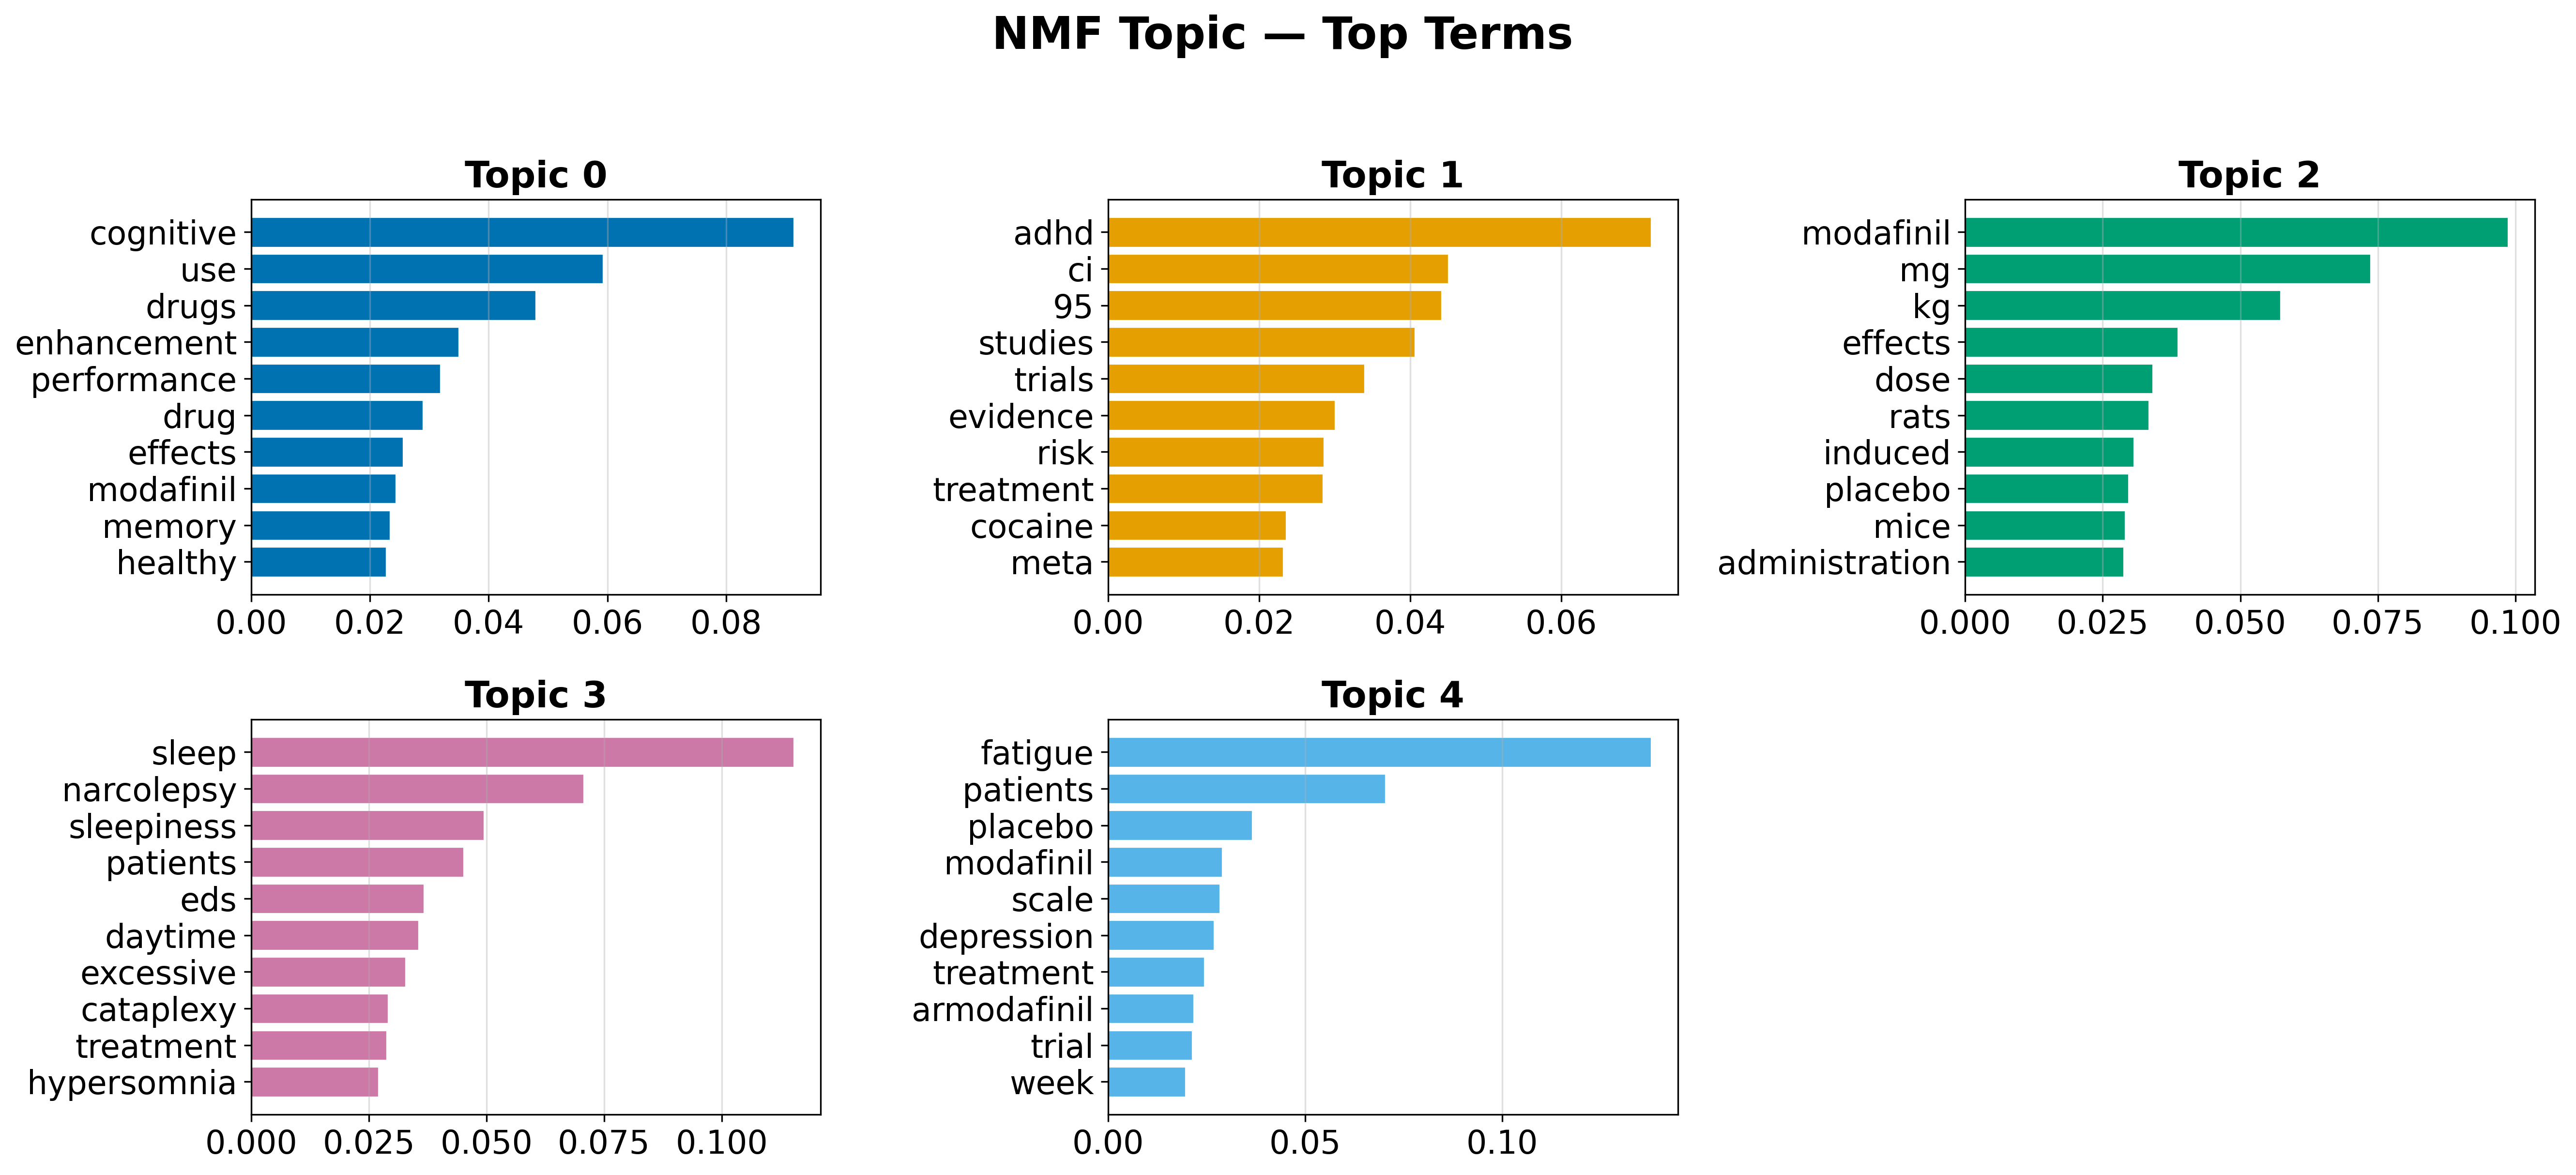
\includegraphics[keepaspectratio,alt={Topic-term bar charts for Modafinil. Each panel shows the top weighted terms for one of 5 NMF topics, with bar length proportional to the topic-term weight in the \textbackslash mathbf\{H\} matrix.}]{../figures/topic_term_bars.png}}\{\{\#fig:topic\_term\_bars\}\}

\subsection{Document Embeddings}\label{document-embeddings}

Offline deterministic embeddings (TF-IDF followed by truncated SVD)
place every document in a shared 50-dimensional vector space. Embedding
the same text twice yields identical vectors, so the derived similarity
matrix, nearest-neighbour lists, clusters, and two-dimensional
projection are all reproducible.

\pandocbounded{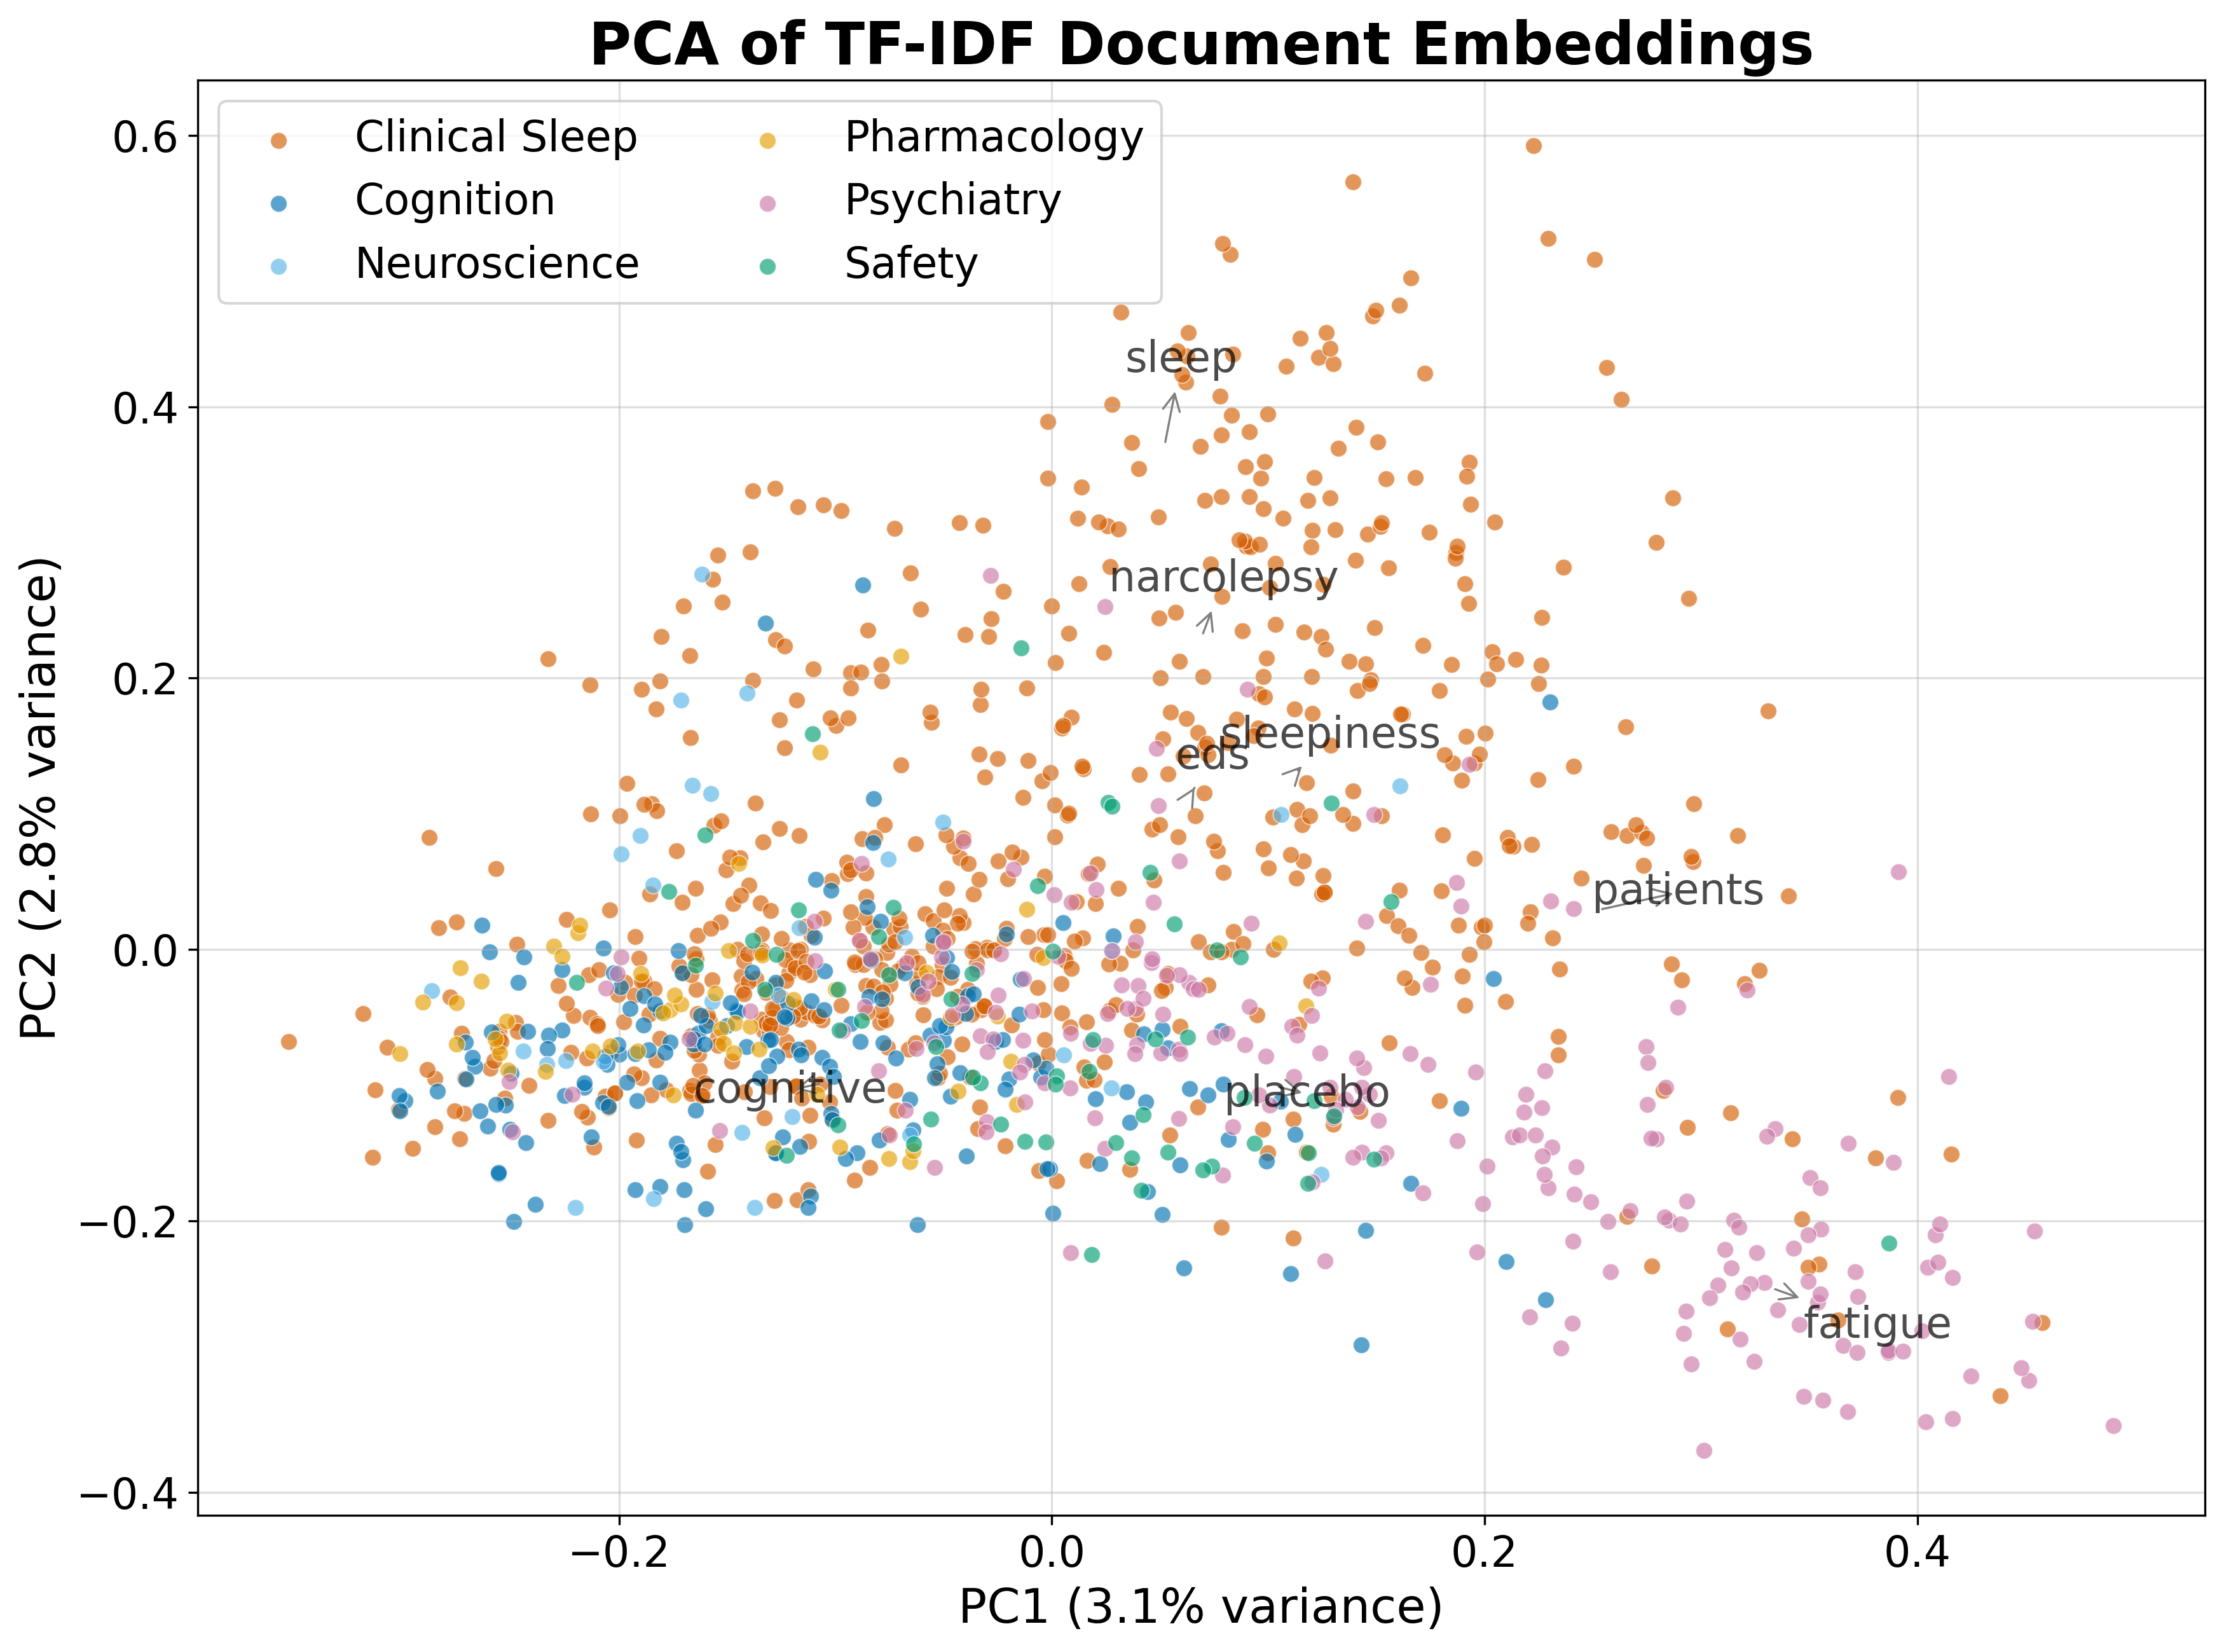
\includegraphics[keepaspectratio,alt={PCA projection of document embeddings for Modafinil. Each point represents one document projected onto the first two principal components of the TF-IDF/SVD embedding. Colours indicate subfield assignment, showing how the topical geography relates to the keyword taxonomy.}]{../figures/pca_embeddings.png}}\{\{\#fig:pca\_embeddings\}\}

\pandocbounded{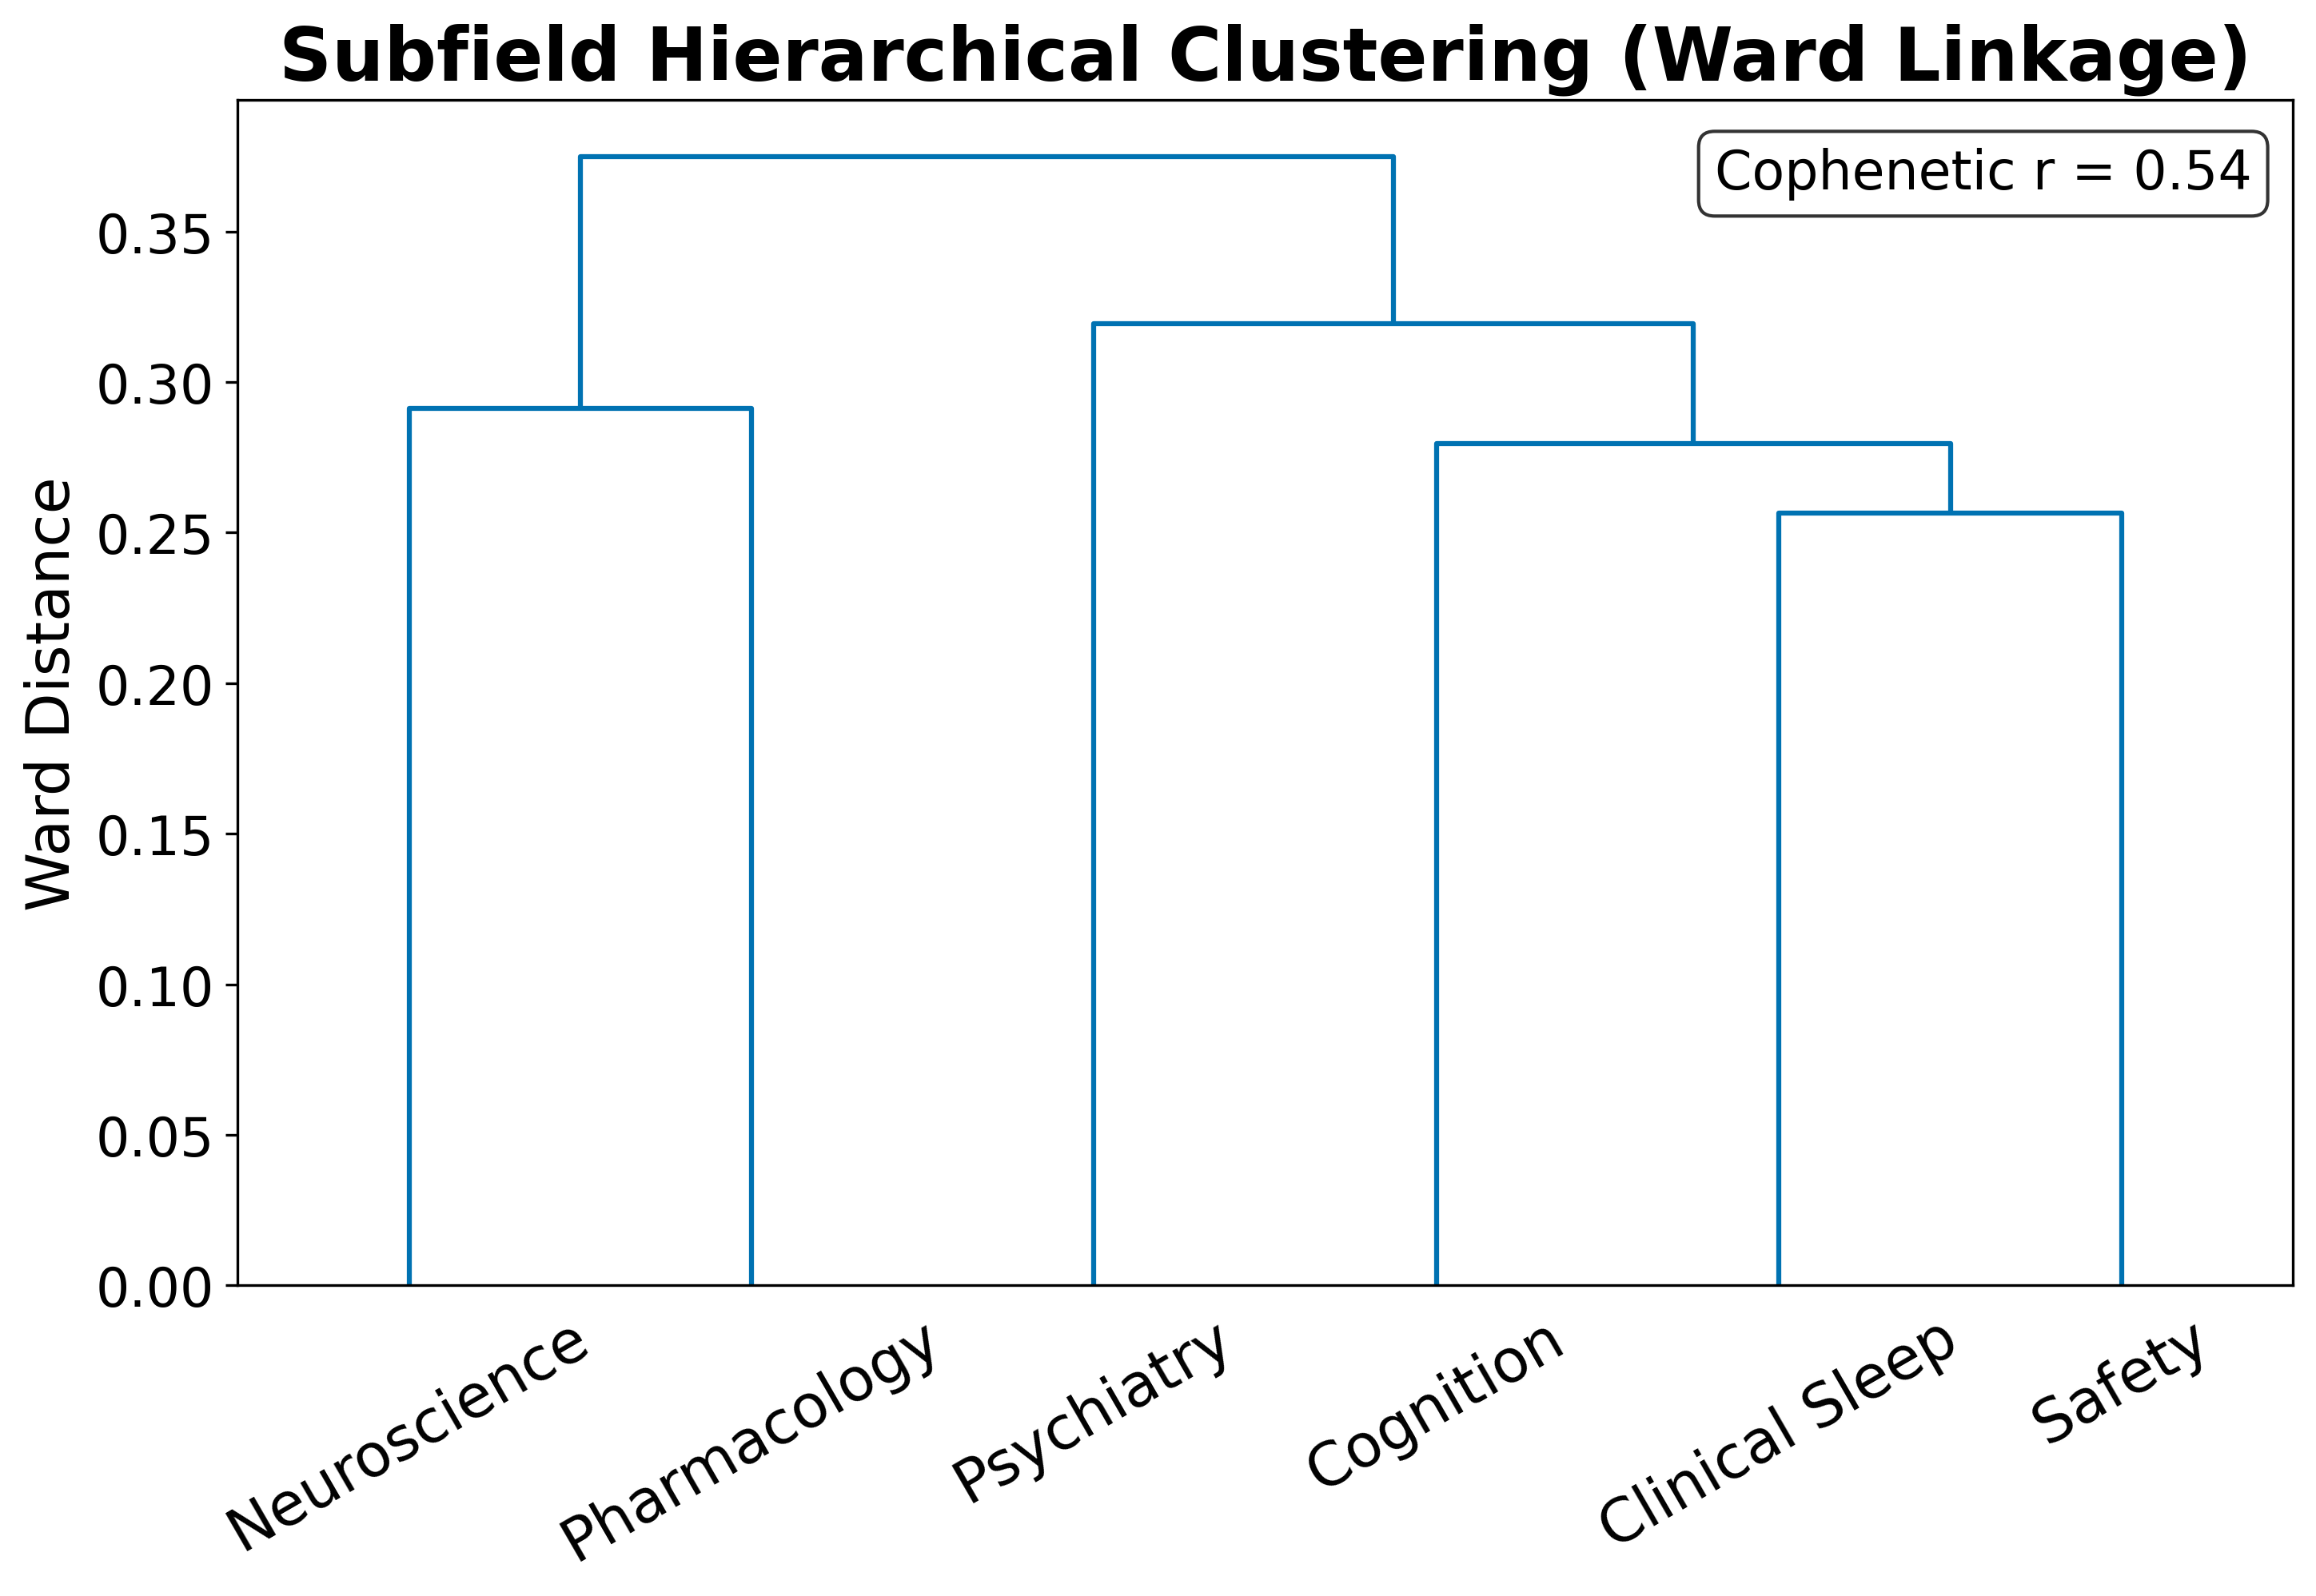
\includegraphics[keepaspectratio,alt={Hierarchical clustering dendrogram of document embeddings. The tree shows the similarity structure of the corpus: documents that join low in the tree are semantically similar, while high-level splits separate the major topical clusters.}]{../figures/dendrogram.png}}\{\{\#fig:dendrogram\}\}

\subsection{Term Analysis}\label{term-analysis}

The TF-IDF term heatmap reveals which terms discriminate between
subfields: terms with high between-subfield variance (rather than high
global mean) are selected for display.

\pandocbounded{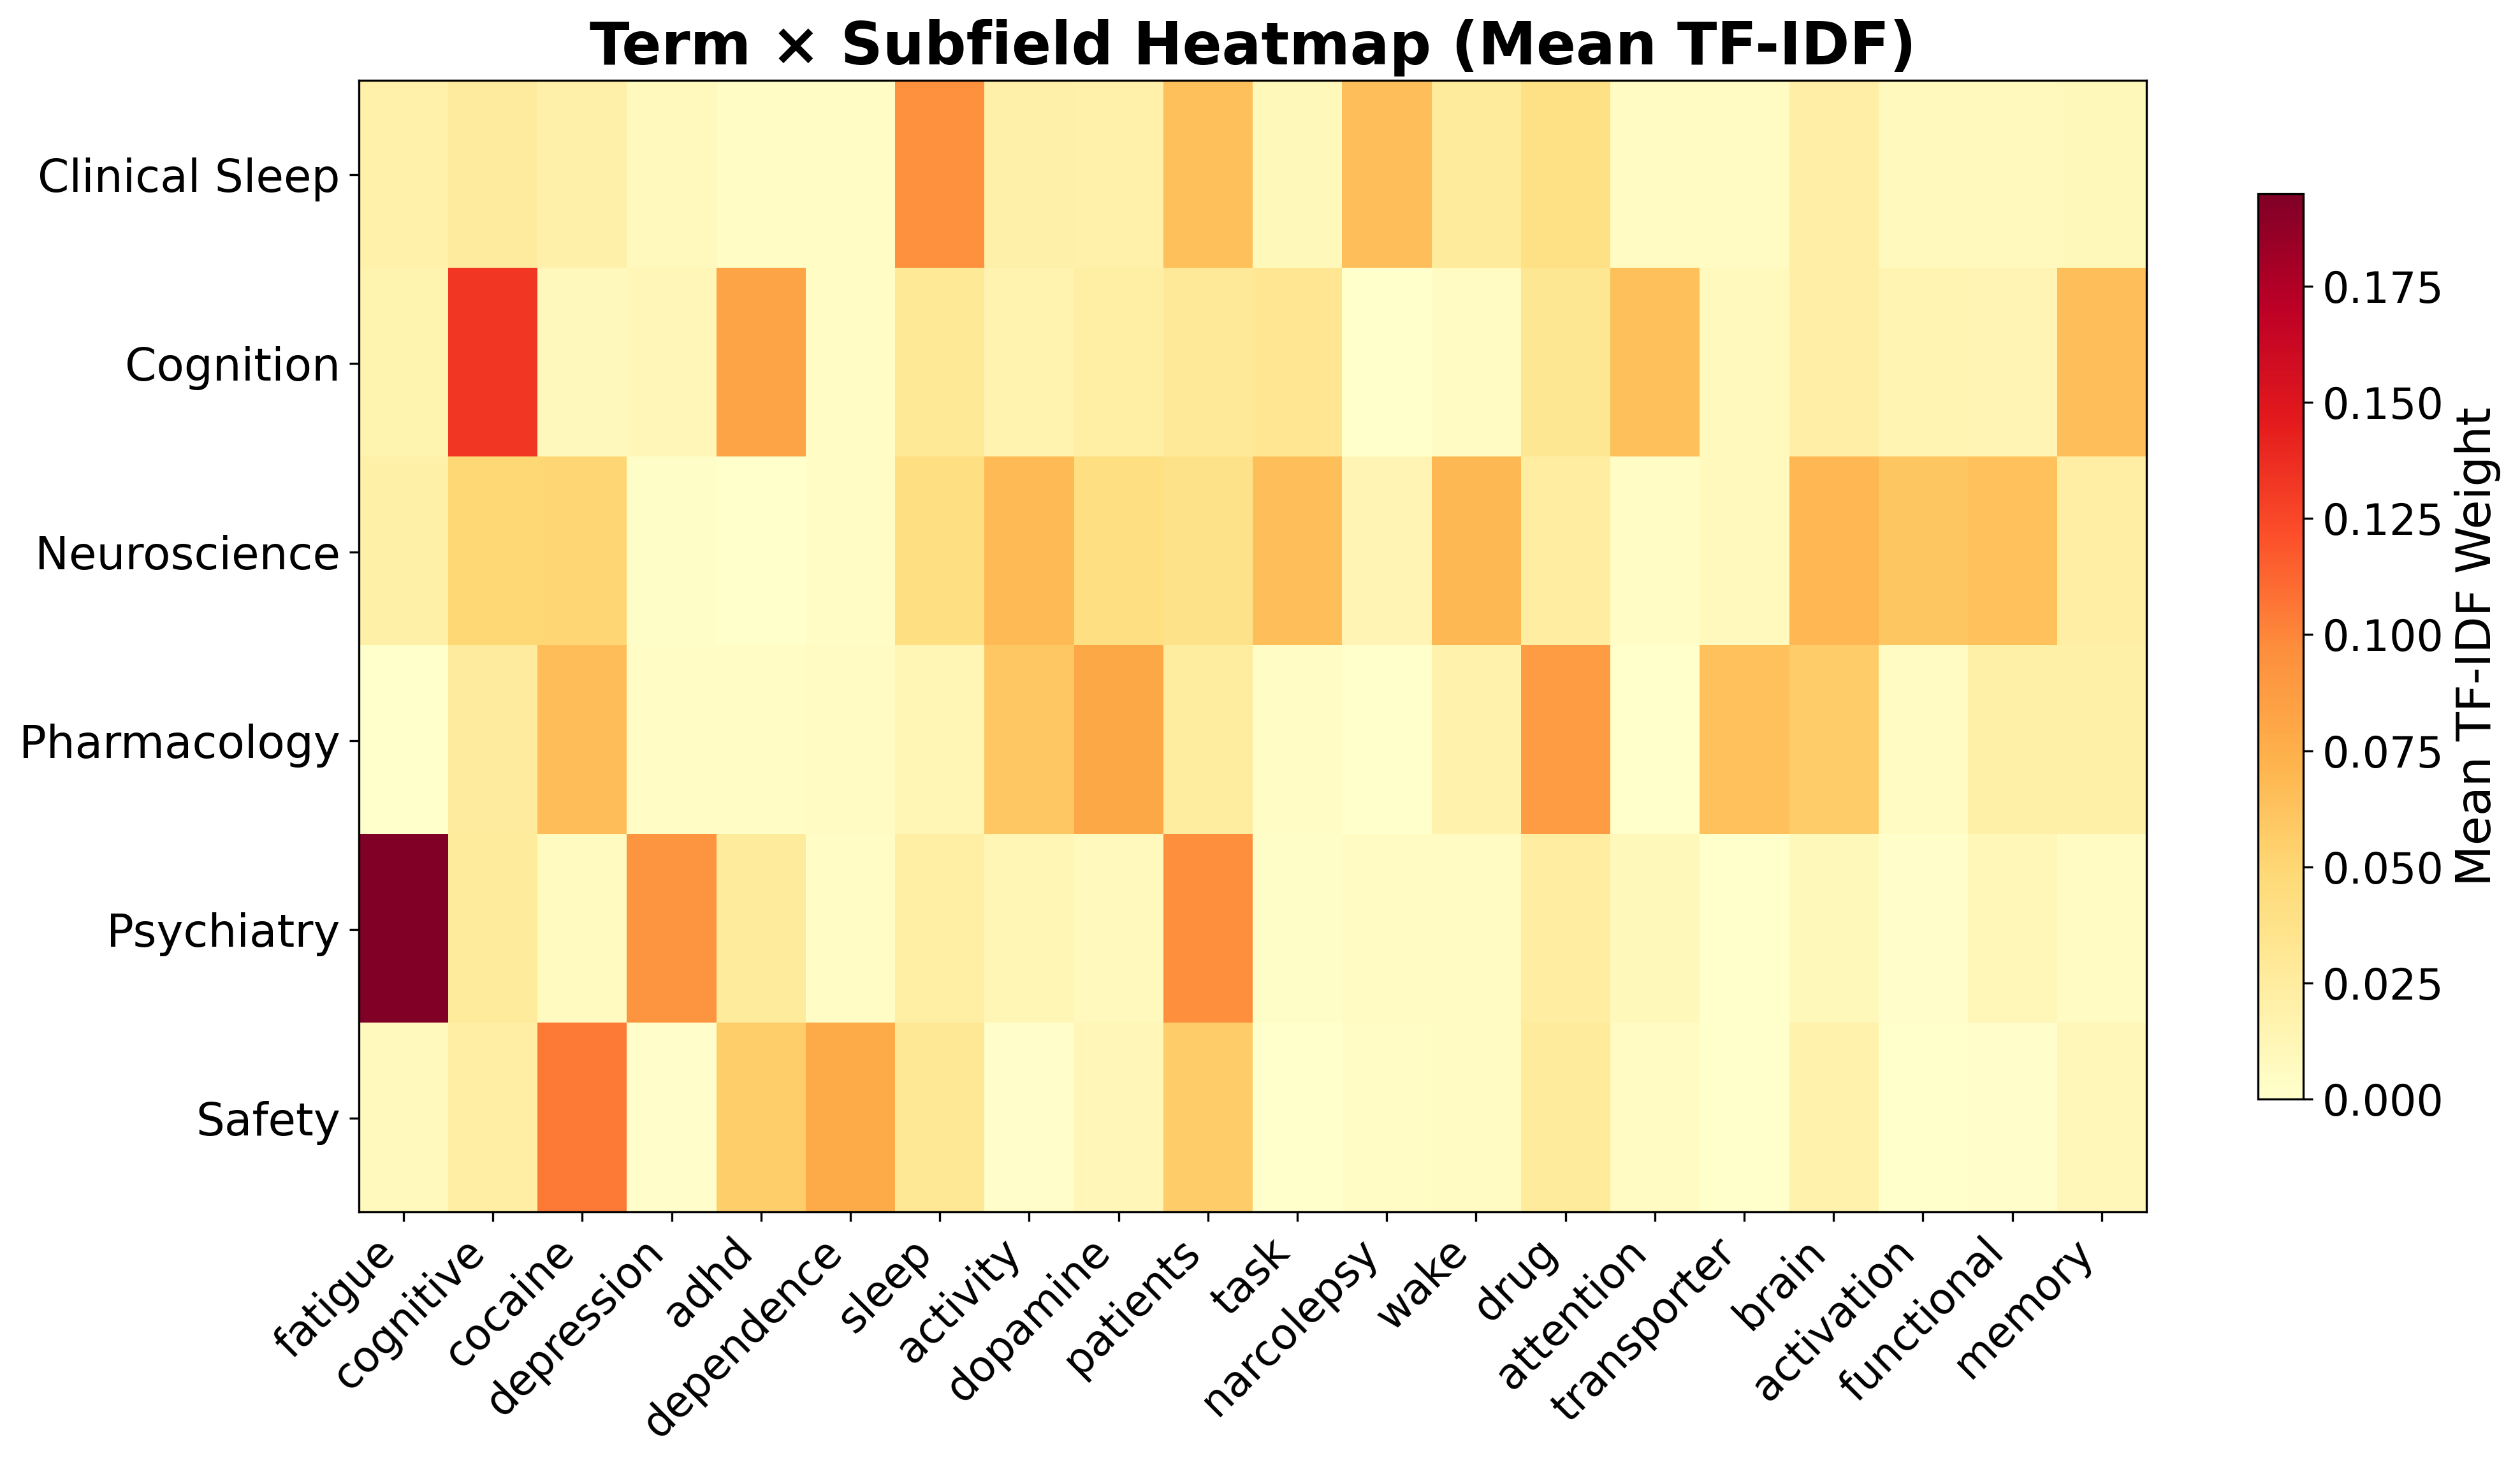
\includegraphics[keepaspectratio,alt={Term heatmap for Modafinil. Each cell shows the mean TF-IDF weight of a term within a subfield. Terms are selected by between-subfield variance to highlight discriminative vocabulary rather than globally frequent terms.}]{../figures/term_heatmap.png}}\{\{\#fig:term\_heatmap\}\}

\subsection{Named Entity Analysis}\label{named-entity-analysis}

Named entity extraction over the 1277 abstracts identified 30 unique
entities. The most frequent entities reflect the clinical and
pharmacological vocabulary of the modafinil literature.

\textbf{Table 4. Top named entities in abstracts.}

{\def\LTcaptype{none} % do not increment counter
\begin{longtable}[]{@{}ll@{}}
\toprule\noalign{}
Entity & Frequency \\
\midrule\noalign{}
\endhead
\bottomrule\noalign{}
\endlastfoot
ADHD & 338 \\
CI & 315 \\
EDS & 258 \\
OSA & 236 \\
MOD & 158 \\
RESULTS & 152 \\
DAT & 133 \\
MS & 132 \\
CONCLUSIONS & 130 \\
ESS & 127 \\
SD & 113 \\
METHODS & 102 \\
CE & 101 \\
MD & 97 \\
IH & 88 \\
\end{longtable}
}

\pandocbounded{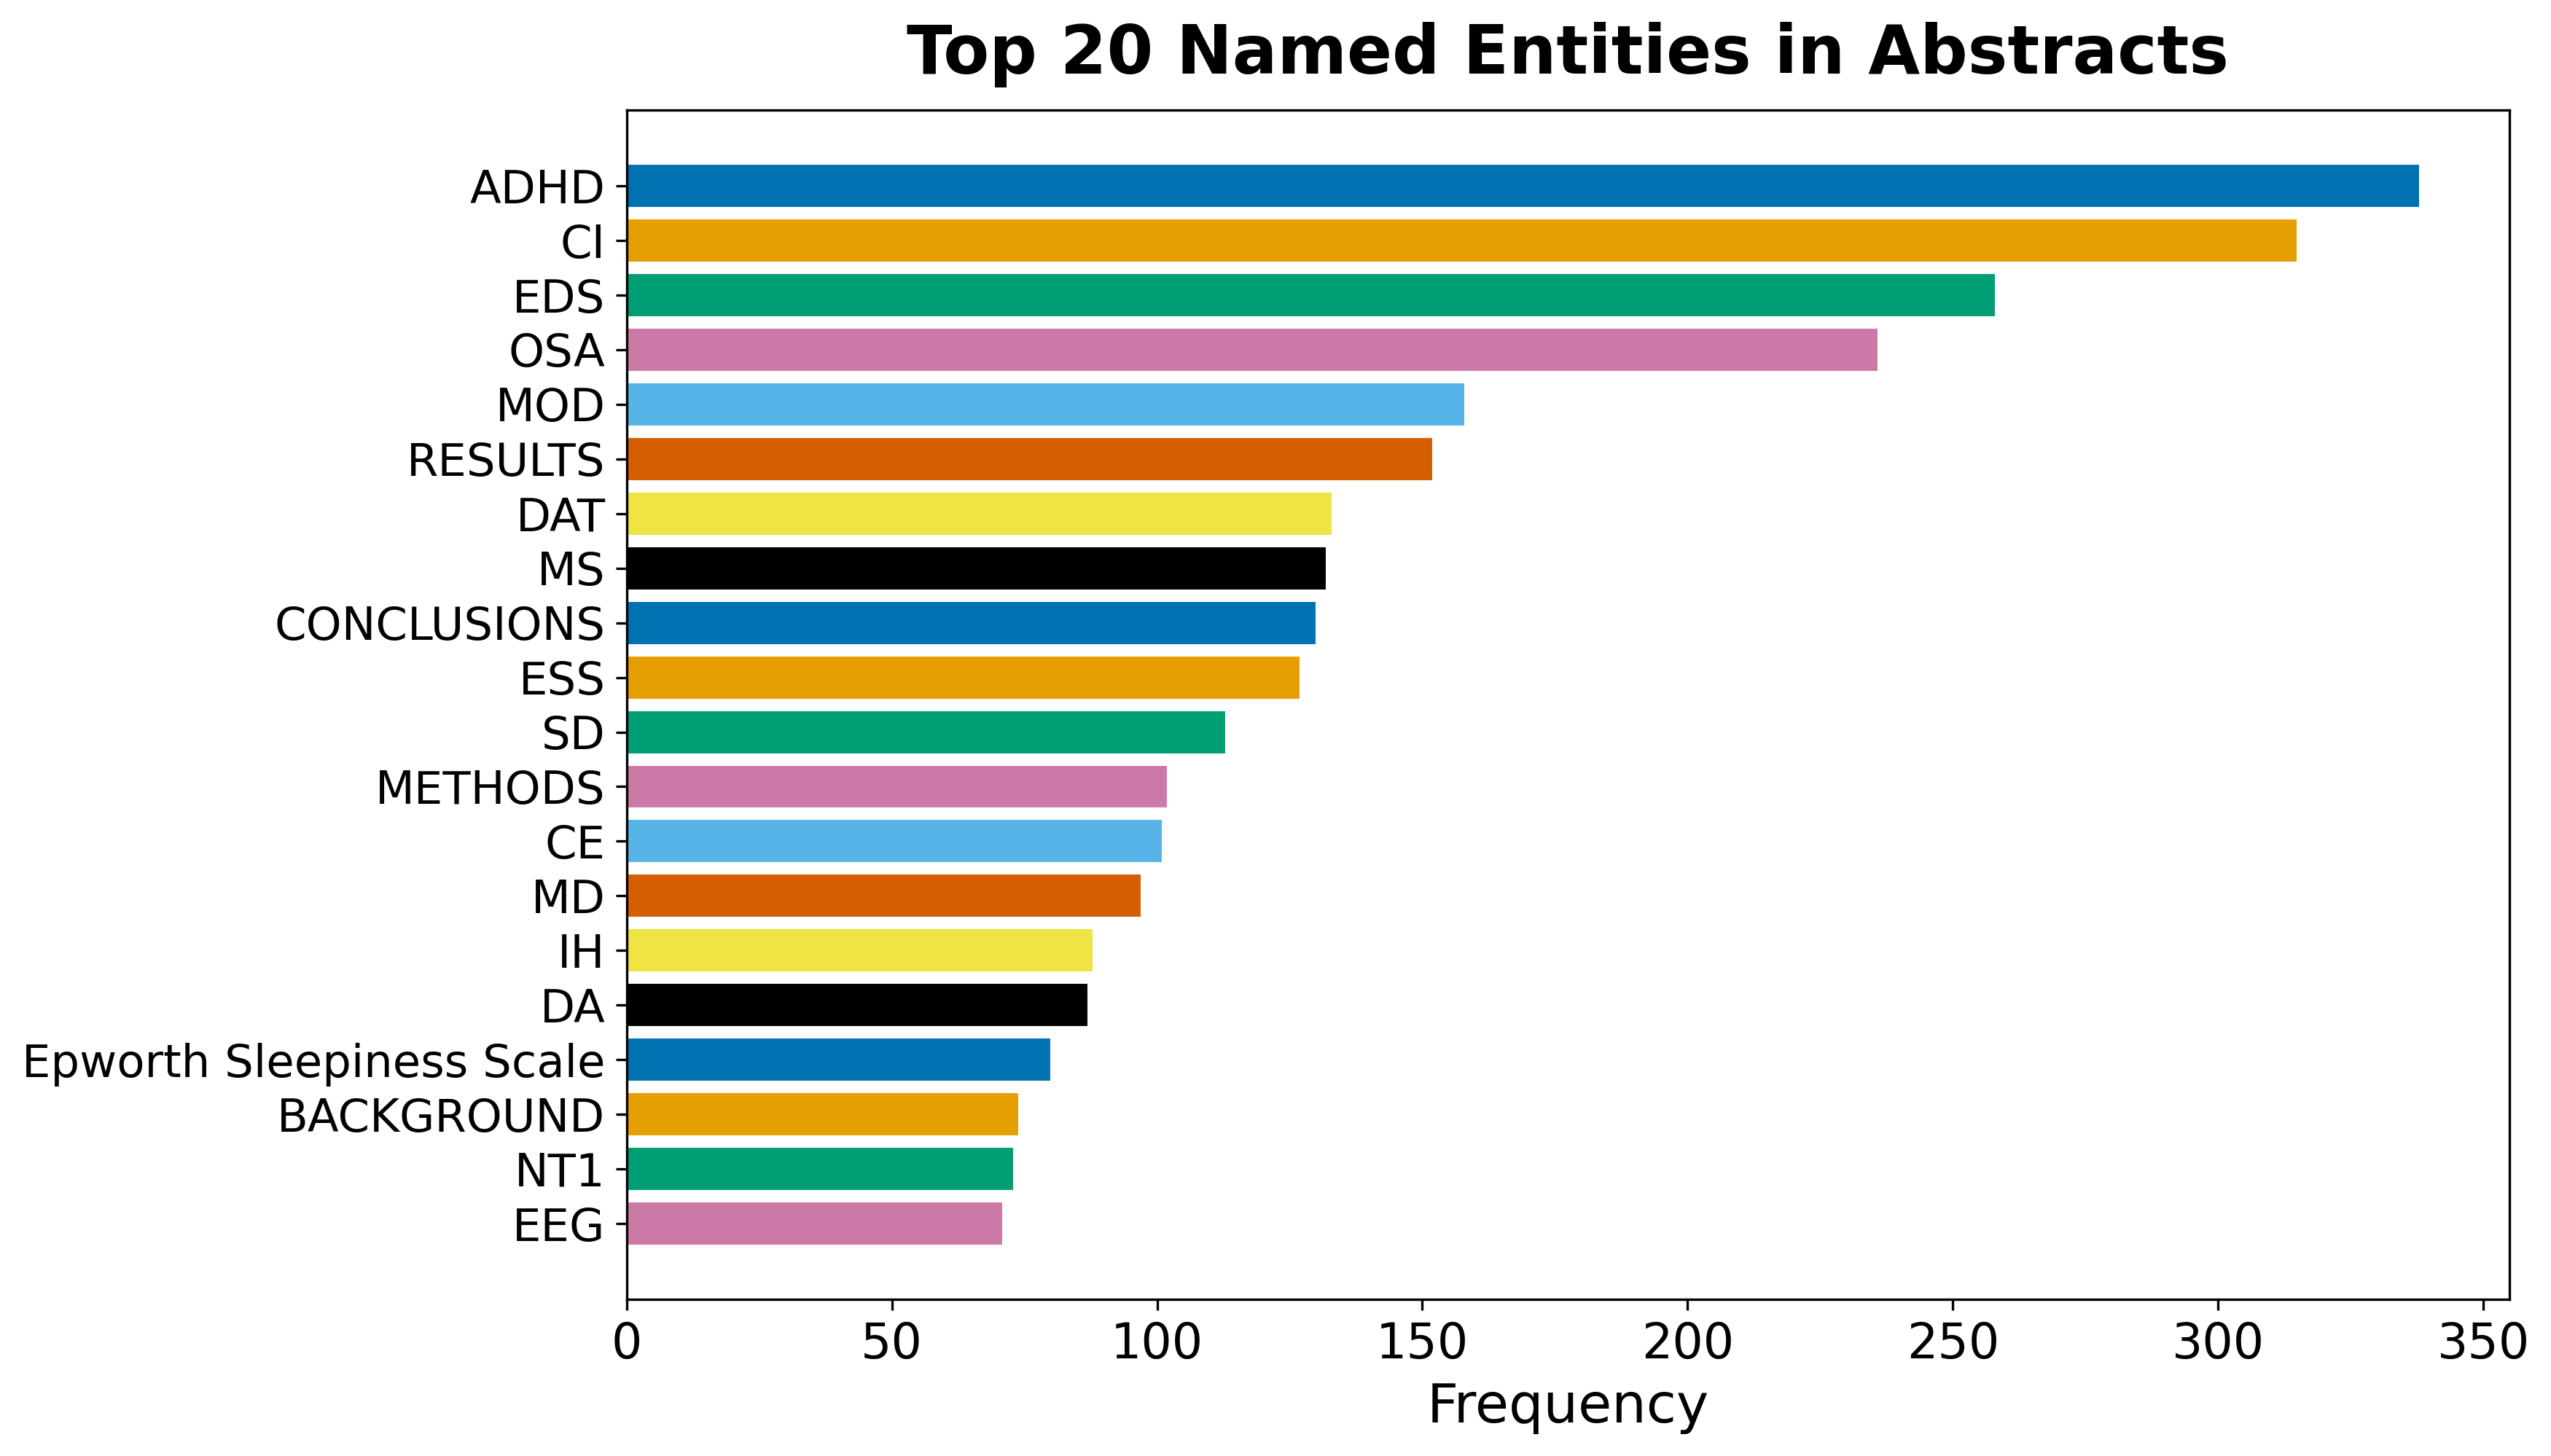
\includegraphics[keepaspectratio,alt={Top named entities for Modafinil. The horizontal bar chart shows the 20 most frequently extracted named entities from abstracts, revealing the dominant drugs, conditions, and concepts in the literature.}]{../figures/entity_bar_chart.png}}\{\{\#fig:entity\_bar\_chart\}\}

\textbf{Table 5. Top keyphrases by TF-IDF score.}

{\def\LTcaptype{none} % do not increment counter
\begin{longtable}[]{@{}ll@{}}
\toprule\noalign{}
Keyphrase & Score \\
\midrule\noalign{}
\endhead
\bottomrule\noalign{}
\endlastfoot
available & 0.3333 \\
abstract & 0.3333 \\
abstract available & 0.3333 \\
content & 0.1053 \\
access & 0.1053 \\
md & 0.0870 \\
jama & 0.0826 \\
cleveland & 0.0763 \\
modafinil & 0.0741 \\
depression & 0.0741 \\
substance & 0.0694 \\
drug & 0.0667 \\
conditions & 0.0667 \\
continuous & 0.0667 \\
continuous flow & 0.0667 \\
\end{longtable}
}

\subsection{Embedding Similarity and
Clustering}\label{embedding-similarity-and-clustering}

The TF-IDF/SVD embeddings place every document in a 50-dimensional
vector space. K-means clustering with \(k = 5\) clusters partitions the
corpus into topically coherent groups. The top similar document pairs,
ranked by cosine similarity, reveal the most closely related works in
the corpus.

\textbf{Table 6. Top 10 most similar document pairs.}

{\def\LTcaptype{none} % do not increment counter
\begin{longtable}[]{@{}
  >{\raggedright\arraybackslash}p{(\linewidth - 4\tabcolsep) * \real{0.3333}}
  >{\raggedright\arraybackslash}p{(\linewidth - 4\tabcolsep) * \real{0.3333}}
  >{\raggedright\arraybackslash}p{(\linewidth - 4\tabcolsep) * \real{0.3333}}@{}}
\toprule\noalign{}
\begin{minipage}[b]{\linewidth}\raggedright
Paper A
\end{minipage} & \begin{minipage}[b]{\linewidth}\raggedright
Paper B
\end{minipage} & \begin{minipage}[b]{\linewidth}\raggedright
Similarity
\end{minipage} \\
\midrule\noalign{}
\endhead
\bottomrule\noalign{}
\endlastfoot
doi:10.1176/appi.ajp.163.12.21 & doi:10.1176/ajp.2006.163.12.21 &
1.0000 \\
doi:10.1176/ajp.2006.163.12.21 & doi:10.1176/appi.ajp.163.12.21 &
1.0000 \\
doi:10.1197/j.aem.2005.08.013 & doi:10.1111/j.1553-2712.2006.t &
1.0000 \\
doi:10.1345/aph.1h302 & doi:10.1136/bcr.08.2011.4652 & 0.9687 \\
doi:10.4088/jcp.09m05900gry & doi:10.1186/s40345-015-0034-0 & 0.9628 \\
doi:10.1016/s2215-0366(18)3026 & doi:10.1016/s2215-0366(25)0006 &
0.9621 \\
doi:10.1345/aph.1h302 & doi:10.1017/neu.2023.6 & 0.9598 \\
doi:10.1111/j.1365-2869.2008.0 & doi:10.3109/07420528.2011.6352 &
0.9538 \\
doi:10.1513/annalsats.202006-6 & doi:10.3760/cma.j.cn112147-202 &
0.9532 \\
doi:10.1345/aph.1h302 & doi:10.1192/bjo.2024.75 & 0.9517 \\
\end{longtable}
}

\pandocbounded{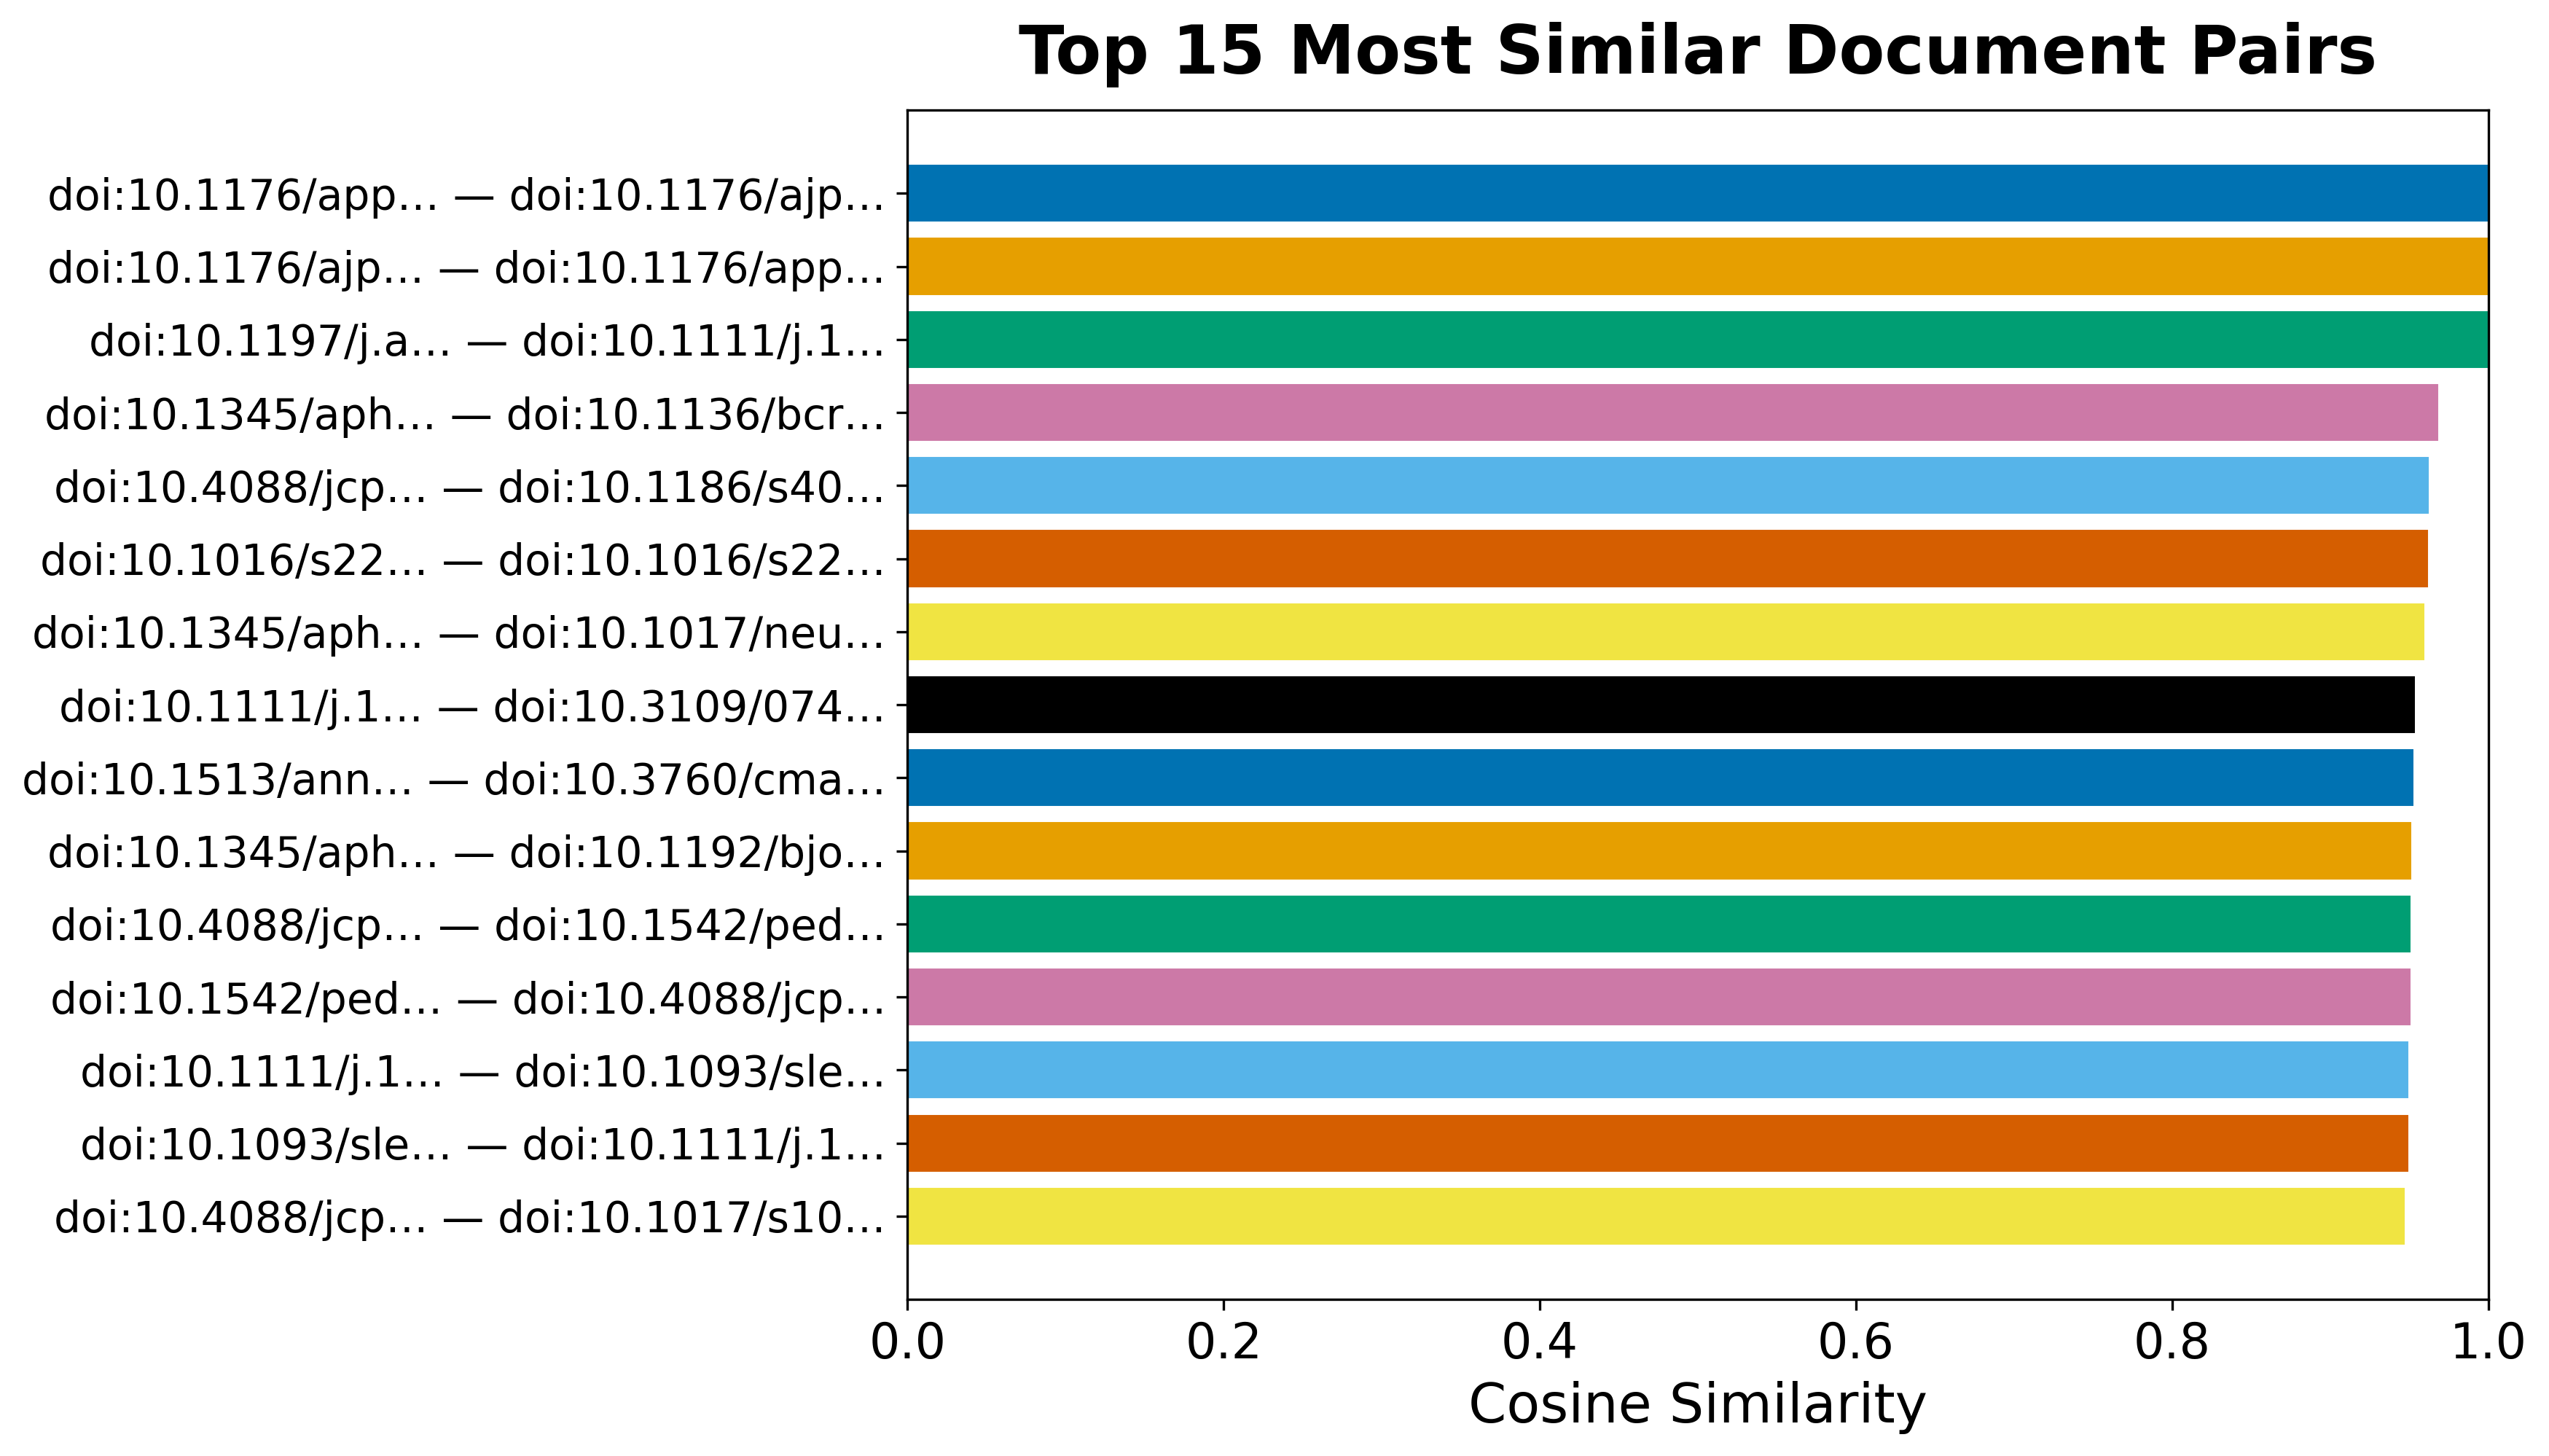
\includegraphics[keepaspectratio,alt={Document similarity for Modafinil. The horizontal bar chart shows the 15 most similar document pairs ranked by cosine similarity of their TF-IDF/SVD embeddings. High-similarity pairs share topical and lexical content.}]{../figures/similarity_heatmap.png}}\{\{\#fig:similarity\_heatmap\}\}

\pandocbounded{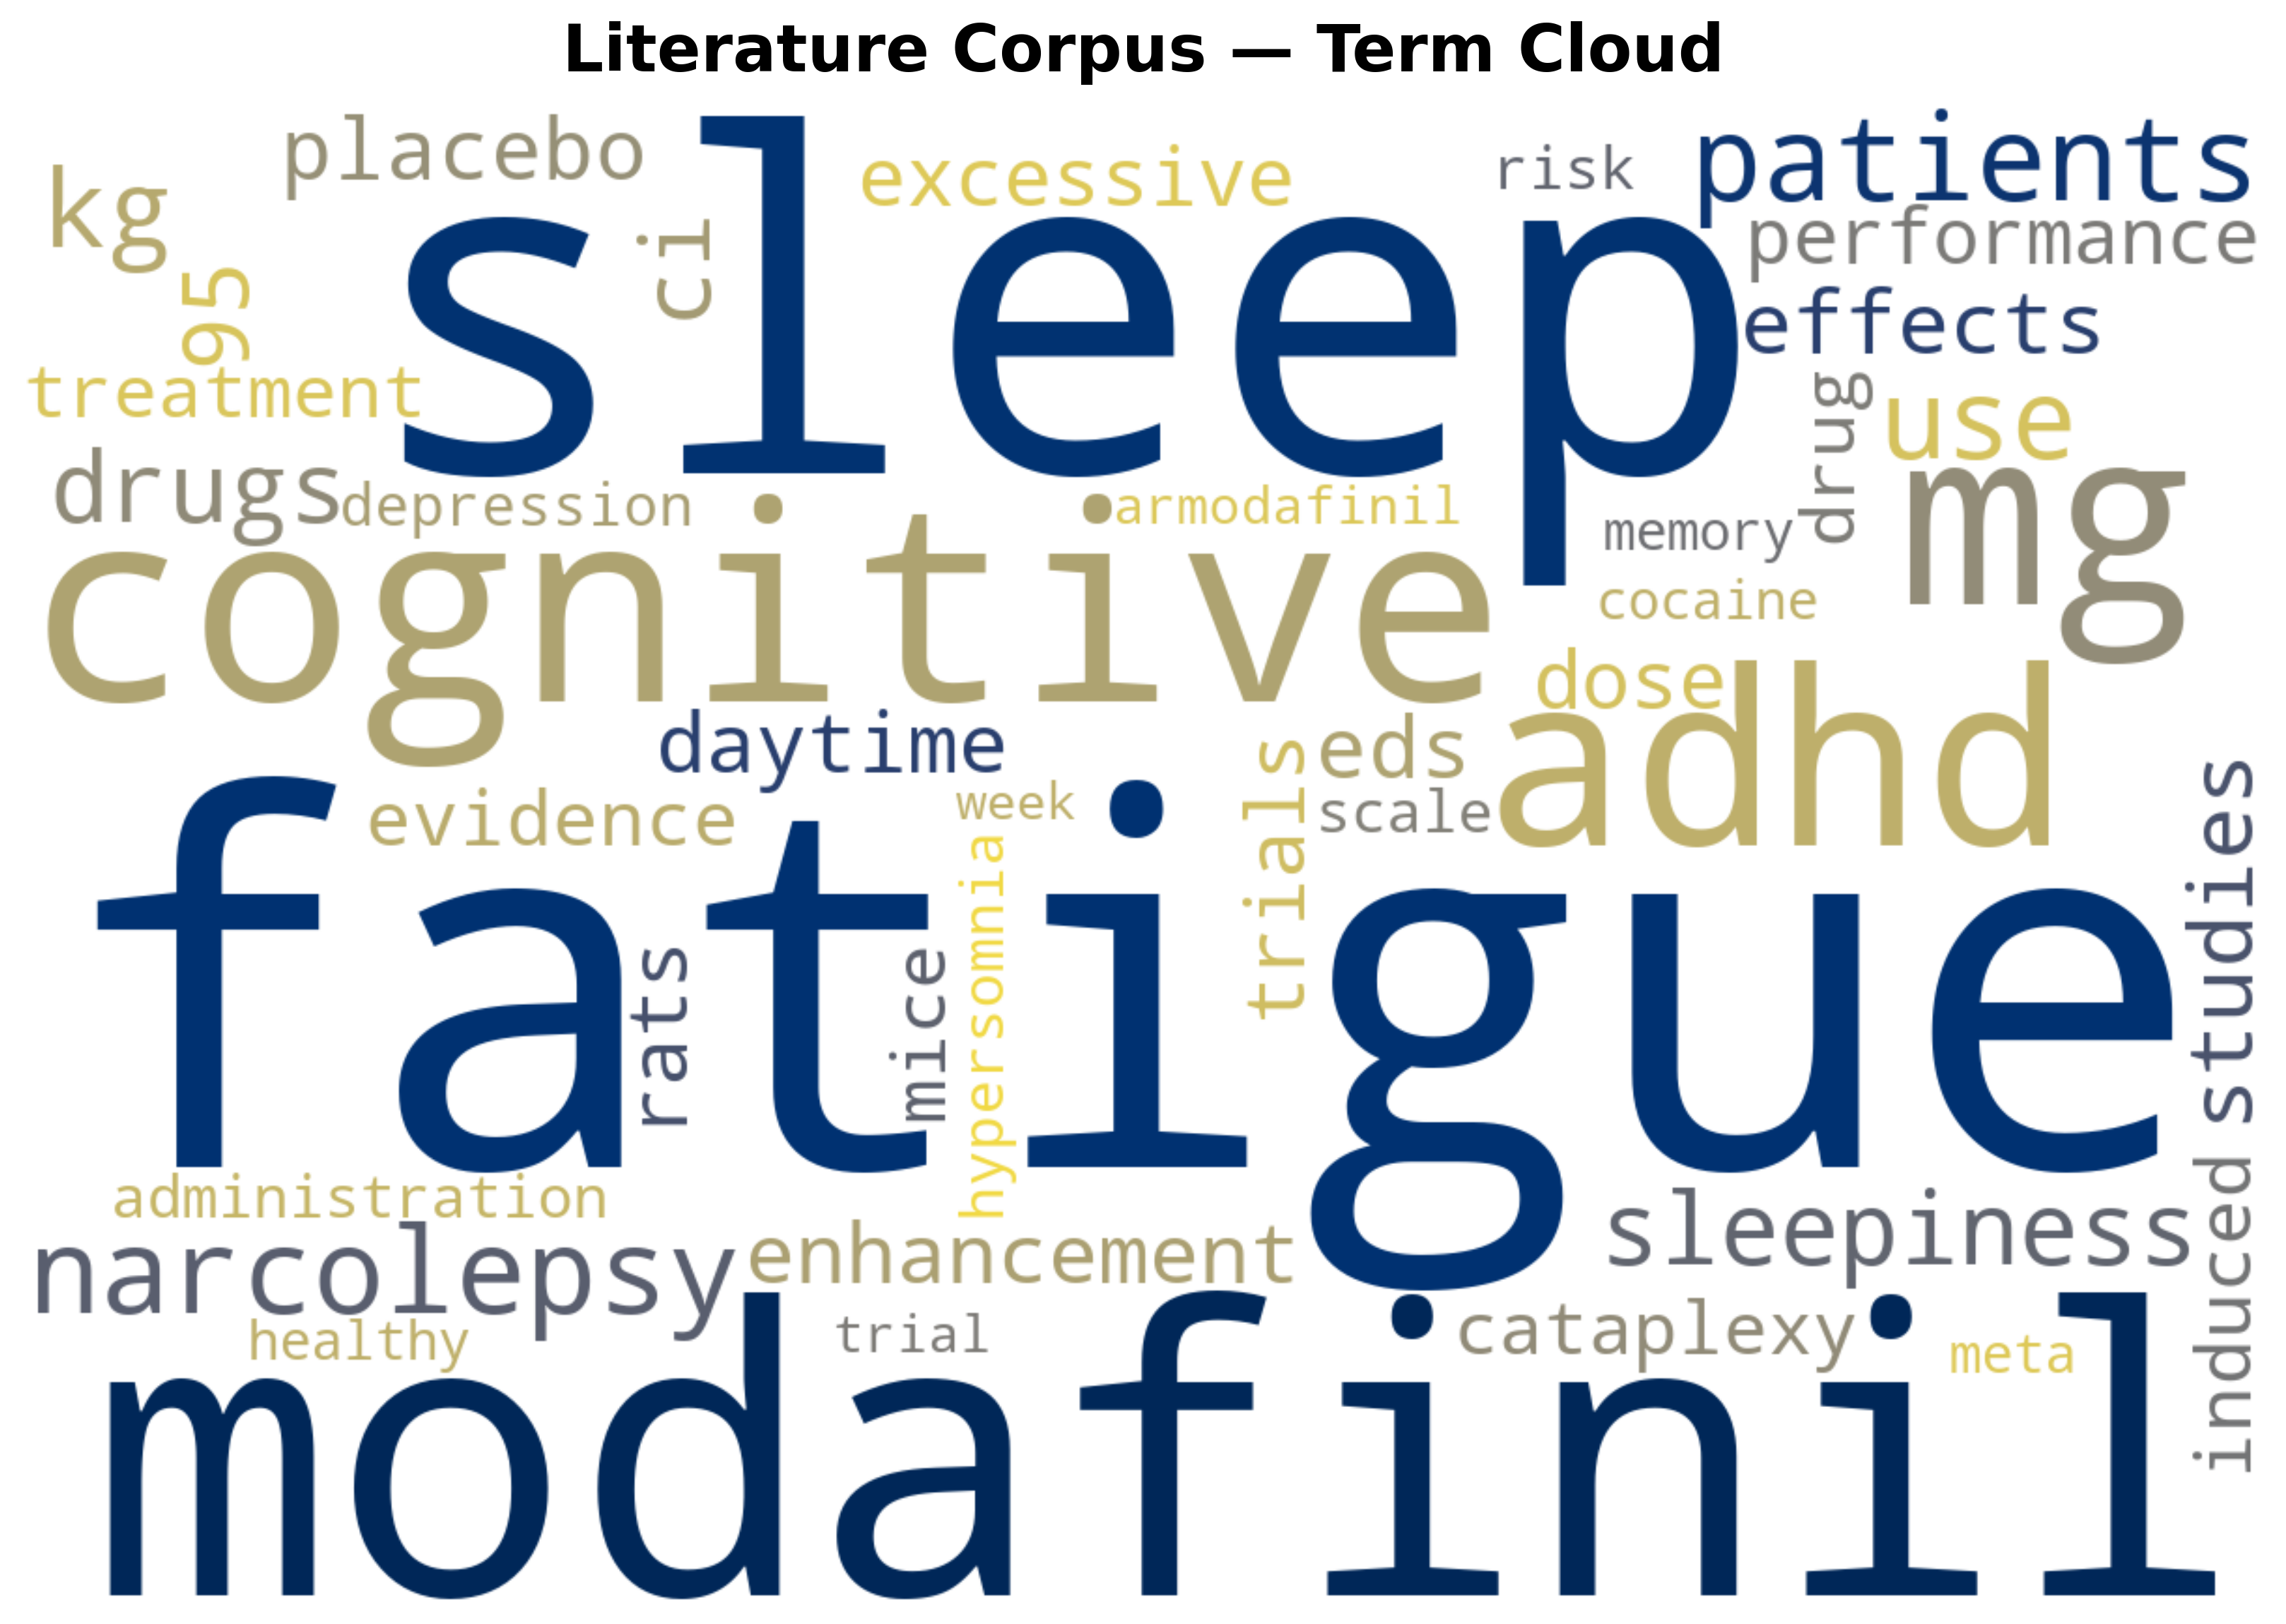
\includegraphics[keepaspectratio,alt={Term cloud for Modafinil. Term sizes are proportional to their TF-IDF weights across the corpus, providing a visual summary of the dominant vocabulary.}]{../figures/word_cloud.png}}\{\{\#fig:word\_cloud\}\}

\pandocbounded{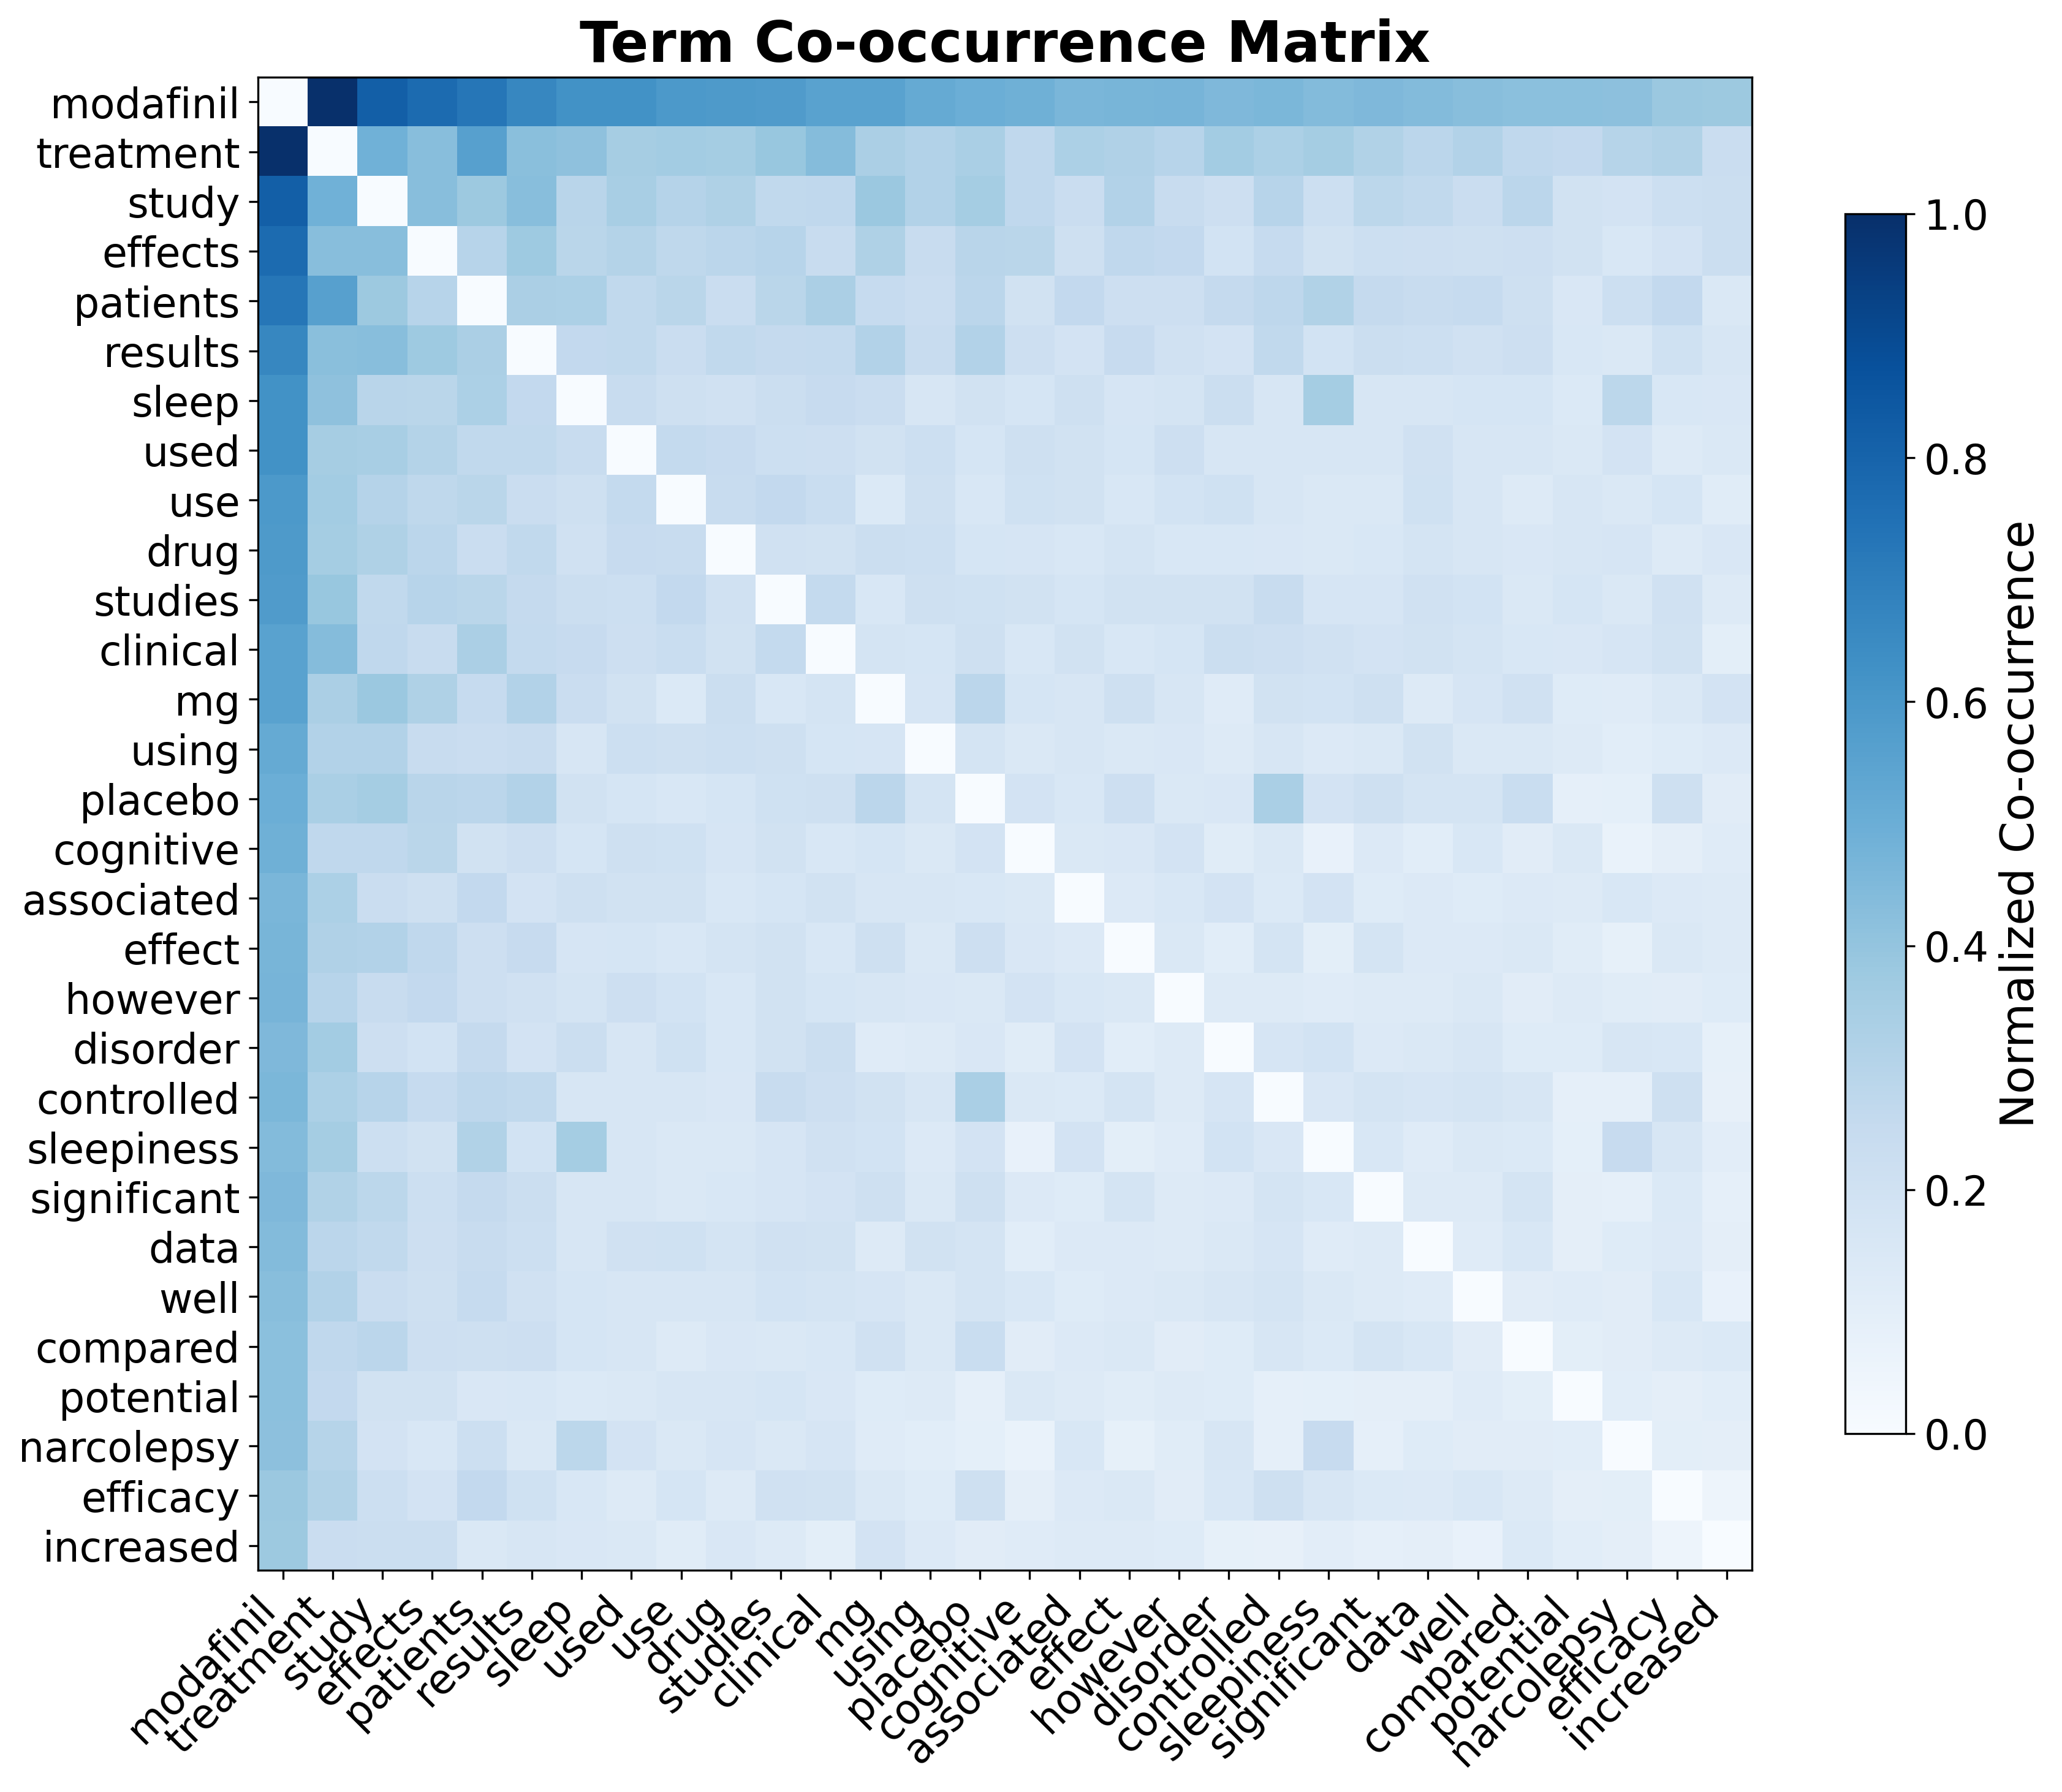
\includegraphics[keepaspectratio,alt={Term co-occurrence matrix for Modafinil. Each cell shows the normalized co-occurrence frequency of two terms within the same document, revealing which concepts tend to appear together in the literature.}]{../figures/cooccurrence_matrix.png}}\{\{\#fig:cooccurrence\_matrix\}\}

These embeddings support semantic retrieval over the corpus and the
visual map of the literature's topical geography.

\newpage

\section{Results: Citation Network}\label{results-citation-network}

\subsection{RQ4: Citation Geometry}\label{rq4-citation-geometry}

Resolving each record's references against the corpus yields an
intra-corpus citation graph (built and analyzed with NetworkX
\citep{hagberg2008exploring}) of 2204 nodes and 8,772 edges across 1371
connected components, with a graph density of 0.18\% and a mean
in-degree of 4.0. Of 38,802 total outgoing references, 22.6\% resolve to
another record inside the corpus --- a resolution rate that reflects how
self-contained the retrieved slice of the literature is rather than the
underlying citation density of any single work.

The citation network has 1377 communities (detected by modularity
optimization), a maximum in-degree of 165 (the most-cited paper within
the corpus), and a maximum out-degree of 145 (the paper that cites the
most other corpus members).

\subsection{Centrality Analysis}\label{centrality-analysis}

Centrality scores (PageRank \citep{page1999pagerank} and HITS) and
modularity-based community detection \citep{clauset2004finding} are
rounded and ranked with a stable tiebreaker so the reported hub and
authority rankings are byte-reproducible across runs despite the
floating-point non-associativity of the underlying iterative solvers.

\textbf{Table 4. Top 5 papers by PageRank.}

{\def\LTcaptype{none} % do not increment counter
\begin{longtable}[]{@{}lll@{}}
\toprule\noalign{}
Rank & DOI & PageRank \\
\midrule\noalign{}
\endhead
\bottomrule\noalign{}
\endlastfoot
1 & 10.1177/026988110001400107 & 0.036955 \\
2 & 10.1212/wnl.54.5.1166 & 0.027240 \\
3 & 10.1523/jneurosci.21-05-01787.2001 & 0.013811 \\
4 & 10.1523/jneurosci.20-22-08620.2000 & 0.011443 \\
5 & 10.4088/jcp.v61n0510 & 0.008104 \\
\end{longtable}
}

\textbf{Table 5. Top 5 authority papers (HITS).}

{\def\LTcaptype{none} % do not increment counter
\begin{longtable}[]{@{}lll@{}}
\toprule\noalign{}
Rank & DOI & Authority \\
\midrule\noalign{}
\endhead
\bottomrule\noalign{}
\endlastfoot
1 & 10.1038/sj.npp.1301534 & 0.017582 \\
2 & 10.1007/s00213-002-1250-8 & 0.015979 \\
3 & 10.1124/jpet.106.106583 & 0.015039 \\
4 & 10.1001/jama.2009.351 & 0.014535 \\
5 & 10.1523/jneurosci.21-05-01787.2001 & 0.014289 \\
\end{longtable}
}

\textbf{Table 6. Top 5 hub papers (HITS).}

{\def\LTcaptype{none} % do not increment counter
\begin{longtable}[]{@{}lll@{}}
\toprule\noalign{}
Rank & DOI & Hub \\
\midrule\noalign{}
\endhead
\bottomrule\noalign{}
\endlastfoot
1 & 10.3389/fnins.2021.656475 & 0.012064 \\
2 & 10.1016/bs.apha.2023.10.006 & 0.011690 \\
3 & 10.1038/sj.npp.1301534 & 0.010781 \\
4 & 10.1080/08897077.2019.1700584 & 0.010618 \\
5 & 10.1007/s00213-013-3232-4 & 0.009971 \\
\end{longtable}
}

The most influential paper by PageRank (DOI 10.1177/026988110001400107)
is a foundational work that anchors the citation structure --- its high
authority score confirms it is frequently cited by other corpus members.
Hub papers, which cite many other corpus members, serve as integrative
reviews or meta-analyses that connect disparate threads of the
literature.

\pandocbounded{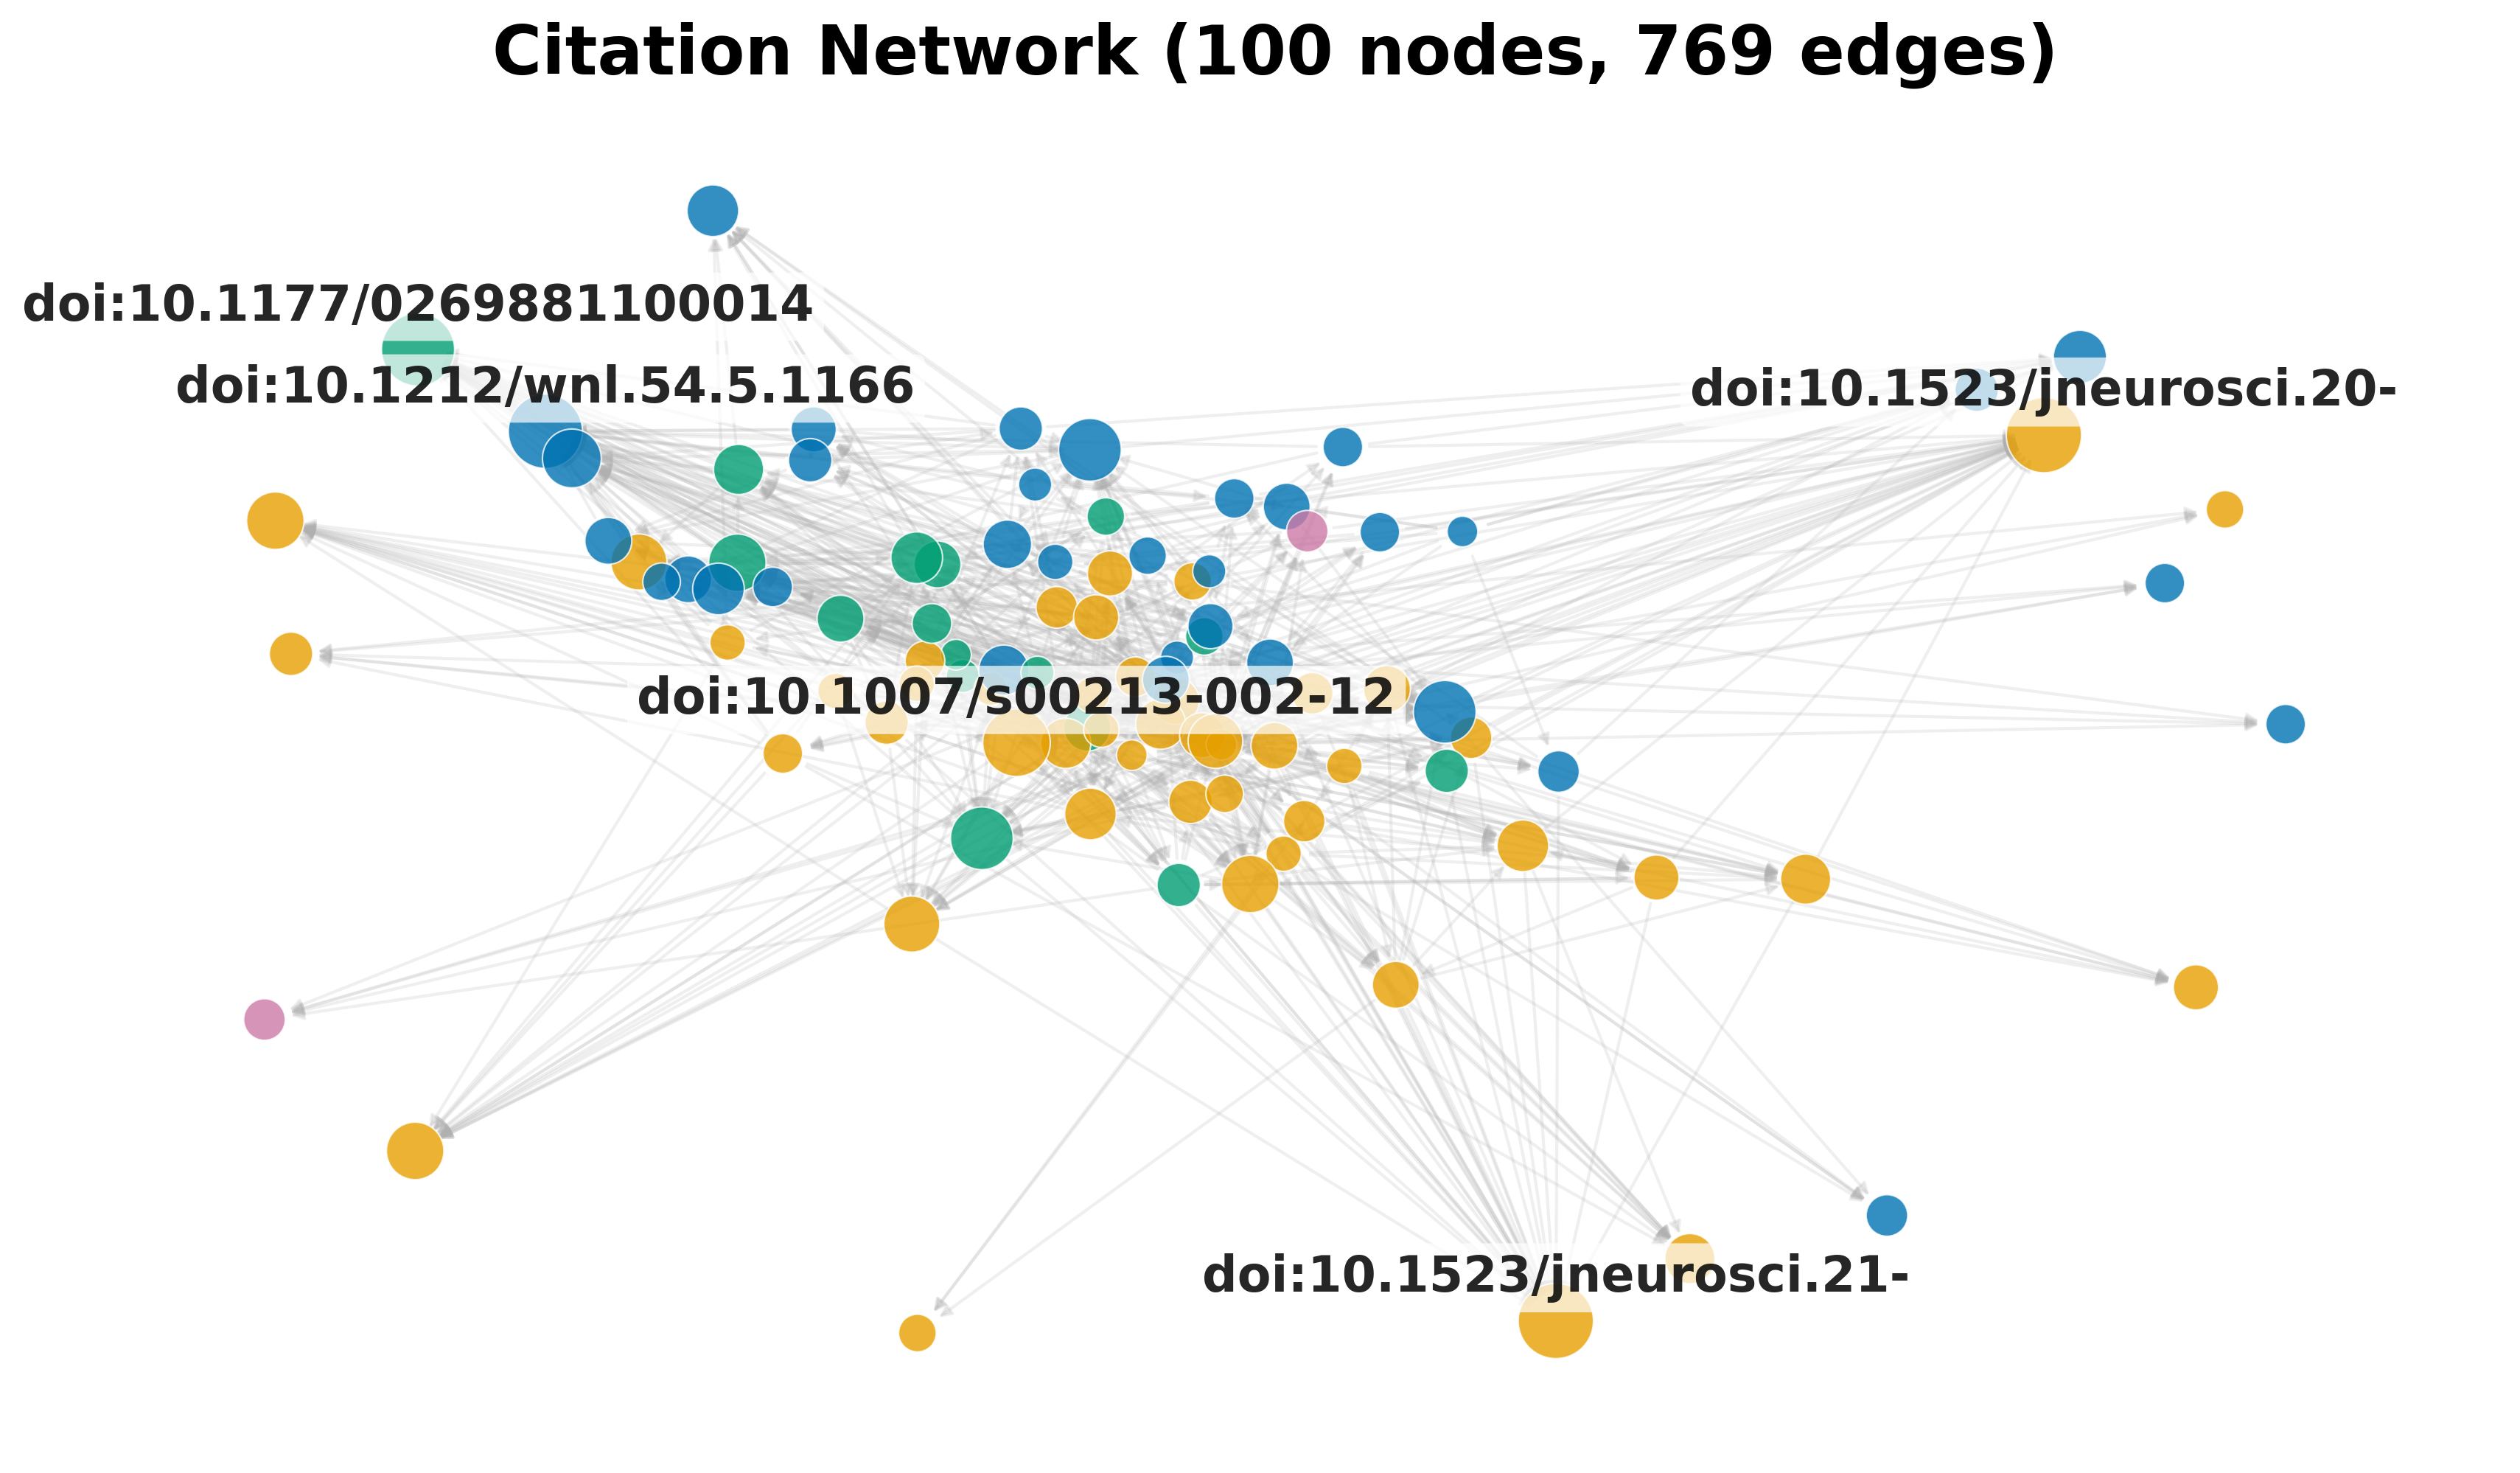
\includegraphics[keepaspectratio,alt={Citation network for Modafinil. Nodes represent papers; directed edges represent citation links. Node colours indicate community membership (1377 communities detected by modularity optimization). Layout uses a spring-based algorithm with a fixed seed for reproducibility.}]{../figures/citation_network.png}}\{\{\#fig:citation\_network\}\}

\pandocbounded{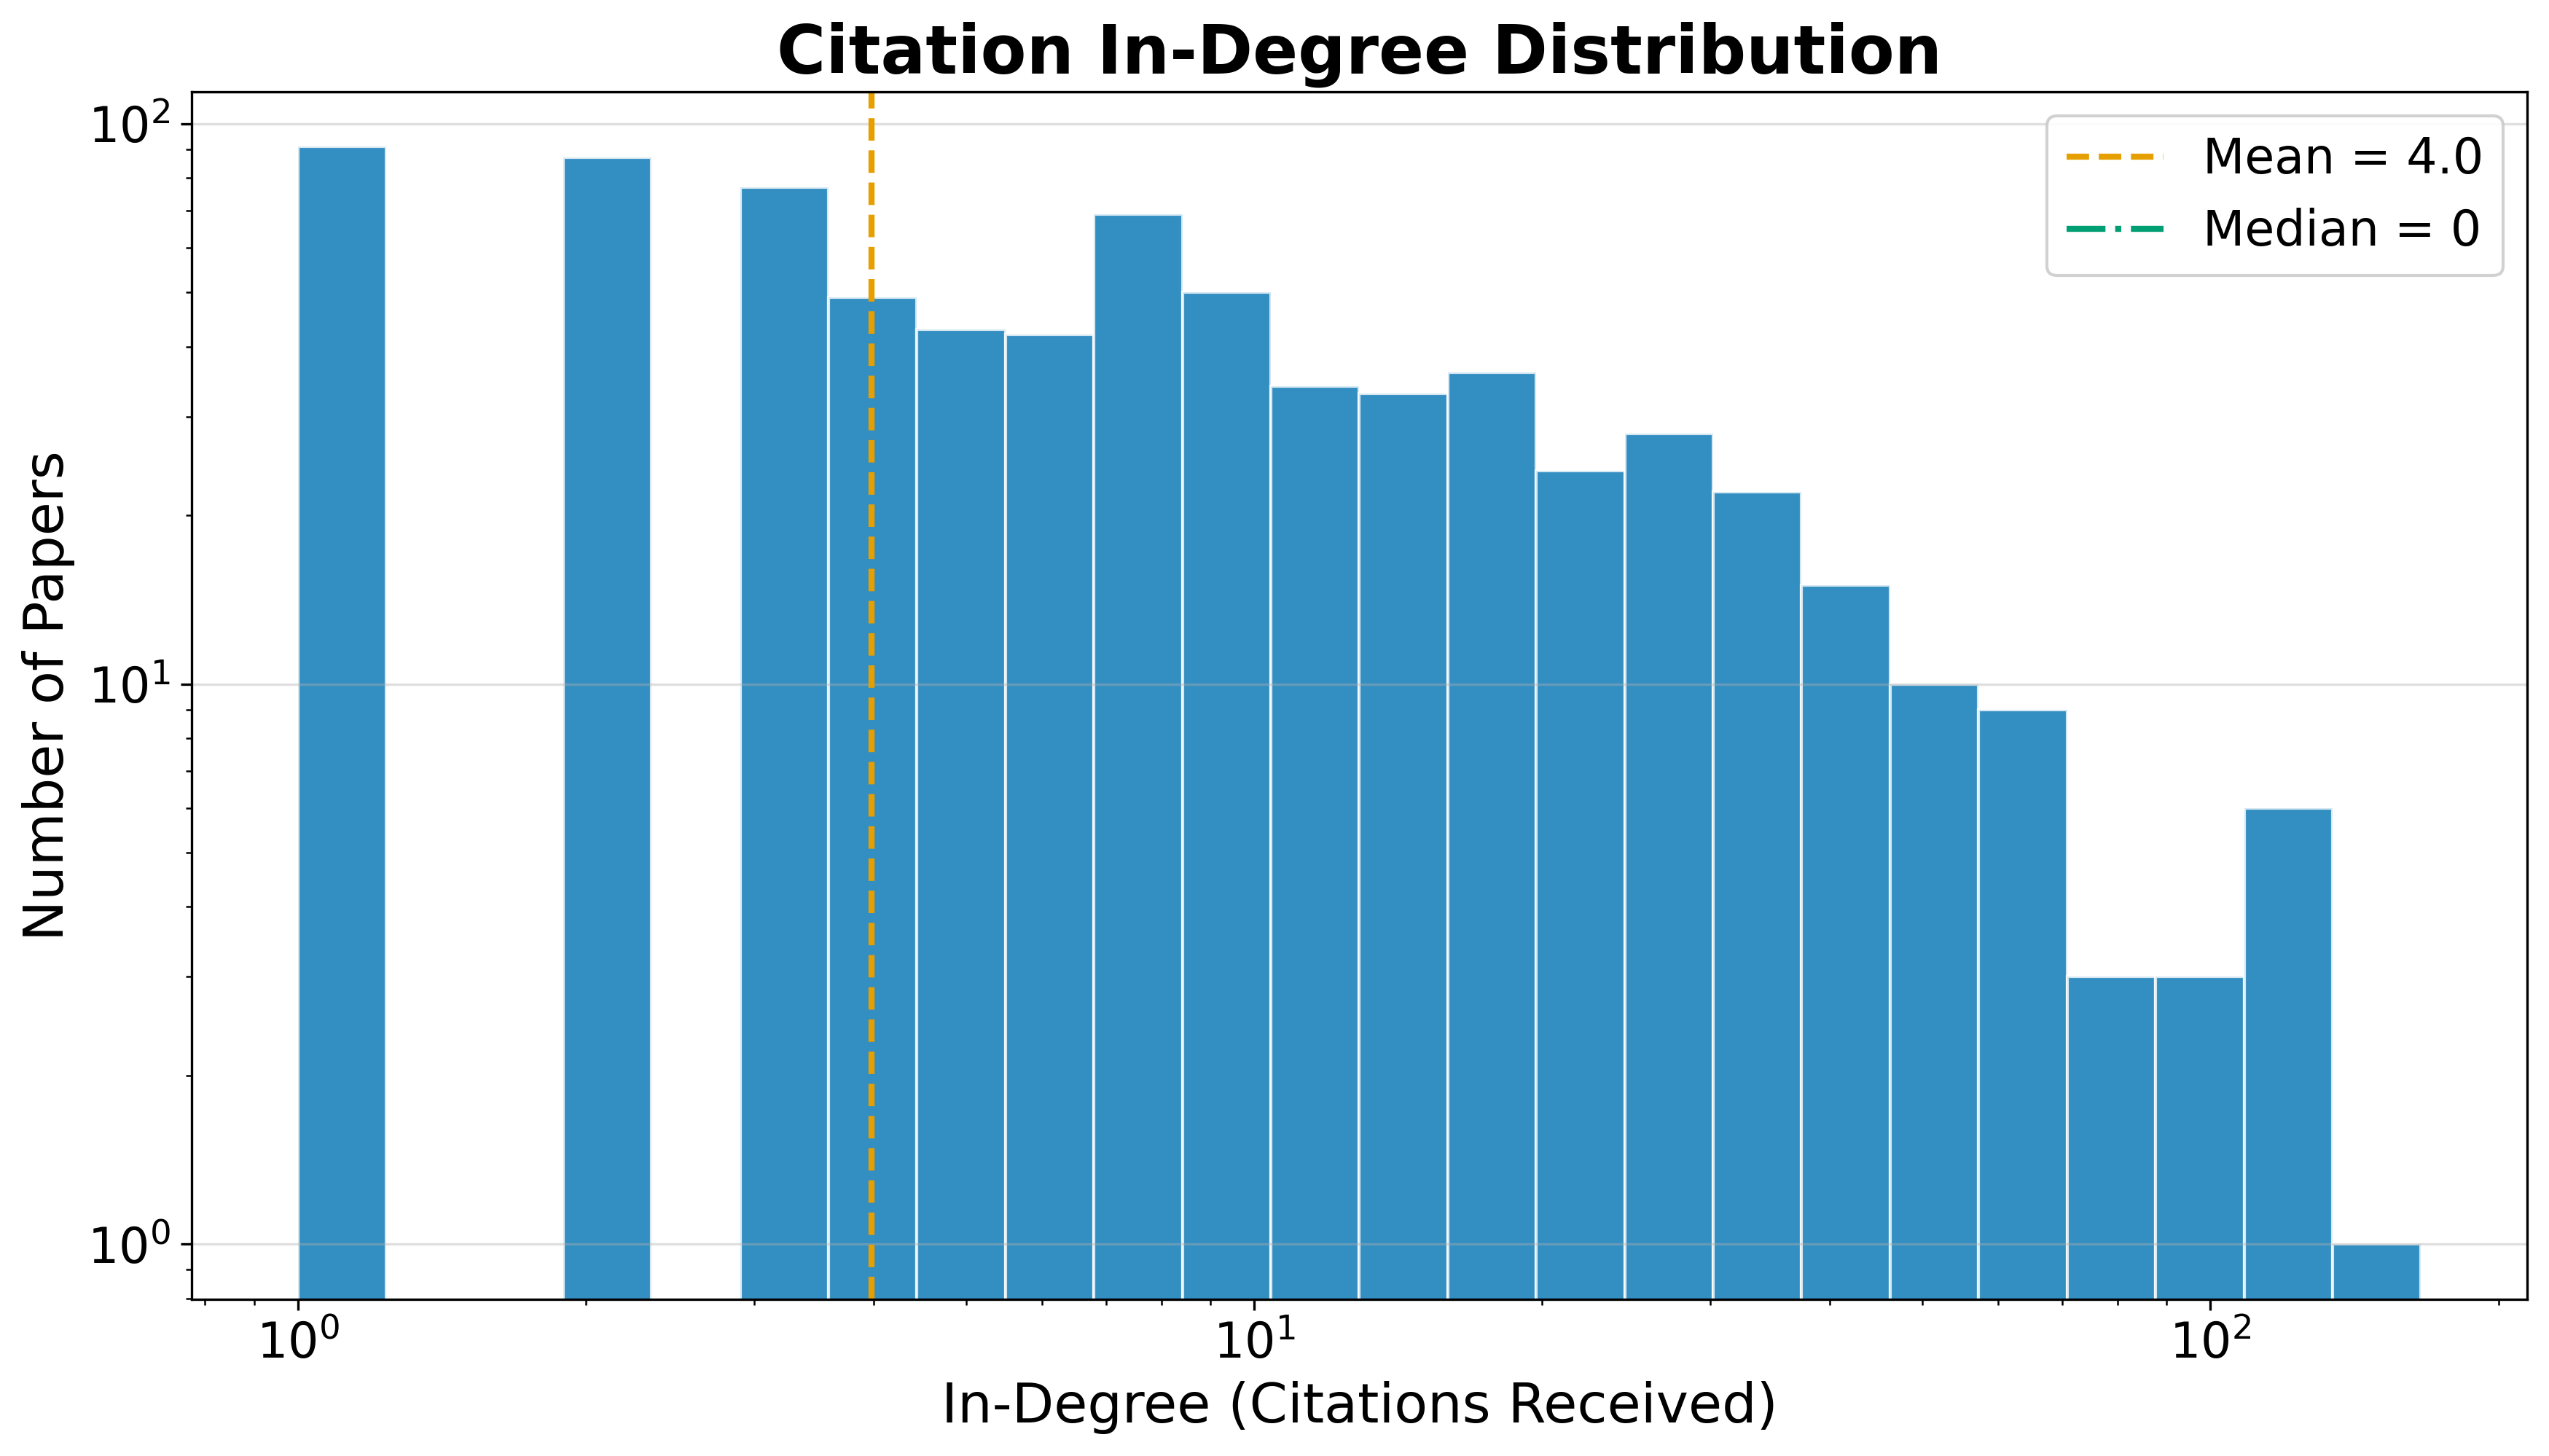
\includegraphics[keepaspectratio,alt={Degree distribution for the Modafinil citation network. The histogram shows the frequency of each in-degree value on a log-linear scale, revealing the heavy-tailed structure characteristic of citation networks.}]{../figures/degree_distribution.png}}\{\{\#fig:degree\_distribution\}\}

The heavy-tailed degree distribution is characteristic of citation
networks: a small number of highly-cited papers anchor the structure,
while the long tail of low-degree nodes represents newer or peripheral
works. The low graph density (0.18\%) reflects the sparsity of
intra-corpus citation links --- most papers cite works outside the
retrieved slice, which is expected for a max-results-capped retrieval.

\subsection{Advanced Network Metrics}\label{advanced-network-metrics}

Beyond PageRank and HITS, the network analysis computes betweenness
centrality (which papers bridge different communities), closeness
centrality (which papers are near all others), degree assortativity (do
highly-cited papers cite other highly-cited papers?), and average
clustering coefficient (how tightly knit are local neighborhoods).

The degree assortativity coefficient is -0.0579, and the average
clustering coefficient is 0.1047. A negative assortativity indicates
that highly-cited papers tend to cite less-cited papers (dissortative
mixing), which is typical of citation networks where review papers (high
in-degree) cite many primary studies (low in-degree).

\textbf{Table 7. Top 5 papers by betweenness centrality.}

{\def\LTcaptype{none} % do not increment counter
\begin{longtable}[]{@{}lll@{}}
\toprule\noalign{}
Rank & DOI & Betweenness \\
\midrule\noalign{}
\endhead
\bottomrule\noalign{}
\endlastfoot
1 & 10.1038/sj.npp.1301534 & 0.006017 \\
2 & 10.4088/jcp.v67n0406 & 0.003330 \\
3 & 10.2165/00003495-200868130-00003 & 0.002036 \\
4 & 10.1124/jpet.106.106583 & 0.001949 \\
5 & 10.1007/s00213-005-0044-1 & 0.001899 \\
\end{longtable}
}

Papers with high betweenness centrality serve as bridges between
different topical communities in the citation network --- their removal
would fragment the graph into disconnected components. These bridging
papers are often review articles or methodological papers that connect
disparate research threads.

\newpage

\section{Conclusion}\label{conclusion}

We have presented a configurable, reproducible meta-analysis template
that turns a single search term into a complete, evidence-bound portrait
of its literature. Applied to \textbf{Modafinil}, it retrieved and
de-duplicated 2302 records across 7 engines (arXiv, OpenAlex, Semantic
Scholar, Crossref, PubMed, SovietRxiv, and ChinaRxiv), classified them
into 6 configurable subfields (with \textbf{Clinical Sleep} dominant at
64.3\%), extracted 5 topics over a 500-feature vocabulary, computed
reproducible document embeddings, mapped the citation network (2204
nodes, 8,772 edges, 1377 communities), and framed 6 hypotheses for
optional evidence scoring.

\subsection{Key Findings}\label{key-findings}

The analysis answers the four research questions posed in the
introduction:

\begin{enumerate}
\def\labelenumi{\arabic{enumi}.}
\item
  \textbf{RQ1 (Growth)}: The modafinil literature spans 26 years
  (2000--2026) and grows at a CAGR of 3.45\%, doubling every 11.3 years.
  The peak year 2025 produced 112 publications, indicating sustained and
  active research interest.
\item
  \textbf{RQ2 (Subfields)}: The 6-bucket taxonomy reveals a
  multi-disciplinary literature dominated by clinical sleep research
  (64.3\%), with significant representation from cognition, psychiatry,
  and pharmacology.
\item
  \textbf{RQ3 (Topics)}: NMF extracted 5 latent topics --- cognitive
  enhancement, ADHD treatment, pharmacological dose-response, sleep
  disorders, and psychiatric fatigue --- that cross-cut the explicit
  subfield taxonomy and reveal the thematic structure of the field.
\item
  \textbf{RQ4 (Citations)}: The citation network of 2204 nodes and 8,772
  edges has a resolution rate of 22.6\%, 1377 communities, and a maximum
  in-degree of

  \begin{enumerate}
  \def\labelenumii{\arabic{enumii}.}
  \setcounter{enumii}{164}
  \tightlist
  \item
    The heavy-tailed degree distribution is characteristic of citation
    networks, with a small number of foundational works anchoring the
    structure.
  \end{enumerate}
\end{enumerate}

\subsection{Architectural
Contribution}\label{architectural-contribution}

The contribution is architectural rather than topical: every
domain-specific value flows from one configuration file and the
pipeline's own outputs into a generated manuscript, so the same
machinery re-targets to any topic by editing configuration alone.
Combined with an offline, deterministic default run, this yields a
\emph{living literature review} --- a synthesis that can be re-executed
on demand as a field evolves, with every number traceable to a
regenerable artifact.

\subsection{Reproducibility}\label{reproducibility}

This manuscript was generated from a live retrieval run using 7 engines.
Every number, table, and figure in this document is injected from a
committed artifact (\breaktt{output/data/*.json},
\breaktt{../figures/*.png}). Re-running the pipeline with the same
configuration reproduces identical data outputs; the 18 figures are
deterministic given fixed seeds, and the manuscript text is regenerated
from the same template. No number in this document was typed by hand.

\newpage

\section{Discussion}\label{discussion}

\subsection{What the Template Is, and Is
Not}\label{what-the-template-is-and-is-not}

The pipeline measures the \emph{shape} of a literature --- its size,
growth, subfield composition, topical structure, citation geometry, and
the hypotheses a field frames. It does not adjudicate scientific truth.
The optional hypothesis scores summarize how the retrieved corpus
\emph{talks about} each claim, weighted by citation influence; they are
an evidence-landscape instrument, not a verdict.

The 5 topics extracted by NMF provide a data-driven complement to the
keyword-based subfield taxonomy. Where the taxonomy assigns each paper
to a single bucket, the topics reveal overlapping thematic structure: a
paper on modafinil's cognitive effects in ADHD patients belongs to the
``Psychiatry'' subfield but also loads on the ``Cognitive Enhancement''
and ``ADHD Treatment'' topics. This multi-resolution view is more
informative than either approach alone.

\subsection{Engine Coverage and Bias}\label{engine-coverage-and-bias}

For this live run, the corpus is dominated by OpenAlex (1,000 records)
and Crossref (1,000 records), with PubMed contributing 986 records and
arXiv contributing 1. Semantic Scholar was rate-limited (HTTP 429) and
returned zero records --- a known limitation of its unauthenticated API
tier. SovietRxiv and ChinaRxiv returned zero records for the modafinil
query, which is expected given their coverage domains.

The max-results cap of 1,000 per engine means the full literature is
larger than the retrieved corpus; the 2302 records represent a bounded
sample rather than the complete literature. The citation network
resolution rate of 22.6\% reflects this: many cited works lie outside
the retrieved slice. Increasing the cap or adding more engines would
improve coverage but also increase runtime and API load.

\subsection{Honest Defaults}\label{honest-defaults}

The committed seed corpus is synthetic (reserved test DOIs, generated
authors) so that the whole pipeline runs offline and byte-identically.
Its numbers demonstrate the machinery; they are not empirical findings
about modafinil. Real claims require a live retrieval run with
regenerated figures, reports, and manuscript variables --- as produced
in this instance.

\subsection{Limitations and
Extensions}\label{limitations-and-extensions}

Several limitations bound the interpretation of results:

\begin{itemize}
\item
  \textbf{Coverage is bounded by the enabled engines and the query.} The
  max-results cap truncates each engine's contribution. Semantic
  Scholar's rate limiting excluded a major source; a Semantic Scholar
  API key would resolve this.
\item
  \textbf{Subfield classification is keyword-based} and only as good as
  the configured taxonomy. Ambiguous papers may be misclassified; a
  classifier based on embeddings or supervised learning could improve
  accuracy.
\item
  \textbf{The default embeddings are lexical} (TF-IDF/SVD). They capture
  term co-occurrence but not semantic similarity; a transformer backend
  (\texttt{embeddings} extra) would improve the quality of
  nearest-neighbour retrieval and clustering.
\item
  \textbf{Hypothesis scoring depends on an external language model.}
  Without Ollama running, scores read \emph{pending}. The scoring is
  also sensitive to prompt design and model choice; the default
  \texttt{gemma3:4b} is a lightweight model suitable for demonstration
  but may miss nuanced assertions.
\item
  \textbf{Abstract coverage is 55.5\%.} Text analytics operate only on
  the subset of records with abstracts, biasing topic models and
  embeddings toward well-indexed sources.
\end{itemize}

Each limitation is a configuration or dependency choice rather than a
change to the core architecture.

\newpage

\section{Appendix A: Tooling and
Reproduction}\label{appendix-a-tooling-and-reproduction}

The pipeline is a two-layer system: generic infrastructure (rendering,
validation, logging) shared across the template monorepo, and
project-local \texttt{src/} modules that implement the meta-analysis.
All numbered \texttt{scripts/} are thin orchestrators that wire I/O,
configuration loading, and logging --- no computational logic resides in
scripts.

\subsection{Reproduce the Offline Default
Run}\label{reproduce-the-offline-default-run}

No network, no language model required:

\begin{Shaded}
\begin{Highlighting}[]
\ExtensionTok{uv}\NormalTok{ run python scripts/generate\_fixture\_corpus.py }\AttributeTok{{-}{-}out}\NormalTok{ output/data/corpus.jsonl}
\ExtensionTok{uv}\NormalTok{ run python scripts/02\_meta\_analysis\_pipeline.py}
\ExtensionTok{uv}\NormalTok{ run python scripts/03\_build\_knowledge\_graph.py }\AttributeTok{{-}{-}max{-}papers}\NormalTok{ 0}
\ExtensionTok{uv}\NormalTok{ run python scripts/04\_generate\_figures.py }\AttributeTok{{-}{-}dpi}\NormalTok{ 300}
\ExtensionTok{uv}\NormalTok{ run python scripts/05\_inject\_variables.py}
\end{Highlighting}
\end{Shaded}

\subsection{Reproduce the Live Run}\label{reproduce-the-live-run}

This manuscript was generated from a live retrieval run. To reproduce:

\begin{Shaded}
\begin{Highlighting}[]
\CommentTok{\# Live search (all 7 engines, max 1000 per engine)}
\ExtensionTok{uv}\NormalTok{ run python scripts/01\_literature\_search.py }\AttributeTok{{-}{-}query}\NormalTok{ modafinil }\AttributeTok{{-}{-}max{-}results}\NormalTok{ 1000 }\AttributeTok{{-}{-}no{-}resume}

\CommentTok{\# Analysis pipeline}
\ExtensionTok{uv}\NormalTok{ run python scripts/02\_meta\_analysis\_pipeline.py}
\ExtensionTok{uv}\NormalTok{ run python scripts/03\_build\_knowledge\_graph.py }\AttributeTok{{-}{-}max{-}papers}\NormalTok{ 0}
\ExtensionTok{uv}\NormalTok{ run python scripts/04\_generate\_figures.py }\AttributeTok{{-}{-}dpi}\NormalTok{ 300}
\ExtensionTok{uv}\NormalTok{ run python scripts/05\_inject\_variables.py}
\ExtensionTok{uv}\NormalTok{ run python scripts/06\_fulltext\_assessment.py}
\end{Highlighting}
\end{Shaded}

\subsection{Re-target to Another
Topic}\label{re-target-to-another-topic}

Edit \breaktt{manuscript/config.yaml} ---
\breaktt{project\_config.search.term}, \texttt{query},
\breaktt{relevance\_keywords}, \breaktt{subfield\_keywords}, and
\breaktt{hypothesis\_definitions} --- then regenerate the seed corpus and
re-run. No code changes are required; the manuscript re-targets through
token injection.

\subsection{Live Retrieval}\label{live-retrieval}

Enable engines under \breaktt{project\_config.search.engines}, supply any
optional credentials (Unpaywall email, Semantic Scholar key), and run
\breaktt{scripts/01\_literature\_search.py}; absent engines degrade to
skipped sources. The CLI supports per-engine skip flags:
\texttt{-\/-skip-arxiv}, \texttt{-\/-skip-s2},
\breaktt{-\/-skip-openalex}, \breaktt{-\/-skip-crossref},
\texttt{-\/-skip-pubmed}, \breaktt{-\/-skip-sovietrxiv},
\breaktt{-\/-skip-chinarxiv}.

\subsection{Test Suite}\label{test-suite}

Every stage is covered by a no-mocks test suite (real computation and
\breaktt{pytest-httpserver} for network adapters) gated at \(\geq 90\%\)
statement coverage on \texttt{src/}. The suite includes 819 tests
covering:

\begin{itemize}
\tightlist
\item
  Record models and serialization (deduplication, canonical ID
  hierarchy)
\item
  All 7 engine clients (arXiv, Semantic Scholar, OpenAlex, Crossref,
  PubMed, SovietRxiv, ChinaRxiv) with pytest-httpserver integration
  tests
\item
  Search runner (multi-engine dispatch, relevance filtering,
  resume/clear, YAML config)
\item
  Bibliometric analysis (subfield classification, temporal metrics,
  TF-IDF, NMF, citation network)
\item
  Knowledge graph (schema, nanopublications, hypothesis scoring, LLM
  extraction)
\item
  Visualization (headless figure generation, style config)
\item
  Manuscript variable computation and injection
\end{itemize}

\newpage

\section{Appendix B: Technical Notes}\label{appendix-b-technical-notes}

\subsection{Determinism}\label{determinism}

All stochastic steps use fixed seeds (seed = 42 for NMF, SVD, and graph
layouts). The fixture corpus, TF-IDF/SVD embeddings, and topic
factorization are byte-stable across runs. Graph centrality scores are
rounded to a fixed precision and ranked with a node-id tiebreaker so
that floating-point non-associativity in iterative solvers cannot
perturb the reported rankings. Record identity uses a content digest
(SHA-1, \breaktt{usedforsecurity=False}) rather than a salted hash, so
de-duplication and corpus byte-stability hold across processes.

\subsection{Data Model}\label{data-model}

Each record is a \texttt{Paper} dataclass with: title, abstract, authors
(list of \texttt{Author}), year, DOI, arXiv ID, Semantic Scholar ID,
OpenAlex ID, venue, citation count, references (list of canonical IDs),
publication date, PDF URL, open-access flag, and full-text source. The
canonical identifier hierarchy governs de-duplication and citation
resolution:

\[
\text{canonical\_id} = \begin{cases}
\texttt{doi:} + \text{normalize}(\text{DOI}) & \text{if DOI present} \\
\texttt{arxiv:} + \text{arXiv\_id} & \text{if arXiv ID present} \\
\texttt{s2:} + \text{S2\_id} & \text{if S2 ID present} \\
\texttt{openalex:} + \text{OpenAlex\_id} & \text{if OpenAlex ID present} \\
\texttt{title:} + \text{SHA1}(\text{title})[:16] & \text{otherwise}
\end{cases}
\]

DOI normalization lower-cases the DOI and strips any
\breaktt{https://doi.org/} or \texttt{dx.doi.org/} prefix, so the same
paper returned by two engines under different case or format variants
merges to a single canonical ID.

\subsection{NMF Mathematics}\label{nmf-mathematics}

Non-negative matrix factorization decomposes the TF-IDF document-term
matrix \(\mathbf{V} \in \mathbb{R}^{m \times n}\) (where \(m\) is the
number of documents and \(n\) is the vocabulary size) into
\(\mathbf{W} \in \mathbb{R}^{m \times k}\) and
\(\mathbf{H} \in \mathbb{R}^{k \times n}\), where \(k\) is the number of
topics (here 5). The factorization minimizes:

\[
\min_{\mathbf{W}, \mathbf{H} \geq 0} \|\mathbf{V} - \mathbf{W} \mathbf{H}\|_F^2
\]

using multiplicative update rules \citep{lee1999learning} with a fixed
random seed for reproducibility. The topic-term matrix \(\mathbf{H}\)
gives the top terms per topic; the document-topic matrix \(\mathbf{W}\)
gives each document's topic loadings.

\subsection{Growth Rate Estimation}\label{growth-rate-estimation}

The compound annual growth rate is:

\[
\text{CAGR} = \left(\frac{N_{\text{end}}}{N_{\text{start}}}\right)^{1/(T_{\text{end}} - T_{\text{start}})} - 1
\]

where \(N_{\text{start}}\) and \(N_{\text{end}}\) are the publication
counts in the first and last years of the corpus, respectively. The
doubling time is \(t_d = \ln(2) / \ln(1 + \text{CAGR})\). For this run:
CAGR = 3.45\%, doubling time = 11.3 years.

\subsection{Configuration Surface}\label{configuration-surface-1}

A single \breaktt{manuscript/config.yaml} controls the search term,
per-engine query and keyword sets, engine enable toggles, subfield
taxonomy, hypotheses, full-text and embedding options, and paper
metadata. This run drew on 7 engines, a 6-bucket taxonomy, and 6
hypotheses.

\subsection{Artifacts}\label{artifacts}

Intermediate and final outputs live under \texttt{output/} and are
disposable and regenerable:

{\def\LTcaptype{none} % do not increment counter
\begin{longtable}[]{@{}
  >{\raggedright\arraybackslash}p{(\linewidth - 4\tabcolsep) * \real{0.3333}}
  >{\raggedright\arraybackslash}p{(\linewidth - 4\tabcolsep) * \real{0.3333}}
  >{\raggedright\arraybackslash}p{(\linewidth - 4\tabcolsep) * \real{0.3333}}@{}}
\toprule\noalign{}
\begin{minipage}[b]{\linewidth}\raggedright
File
\end{minipage} & \begin{minipage}[b]{\linewidth}\raggedright
Stage
\end{minipage} & \begin{minipage}[b]{\linewidth}\raggedright
Description
\end{minipage} \\
\midrule\noalign{}
\endhead
\bottomrule\noalign{}
\endlastfoot
\texttt{corpus.jsonl} & 01 & De-duplicated corpus (2302 records) \\
\breaktt{temporal\_analysis.json} & 02 & Year counts, CAGR, doubling
time, peak year \\
\breaktt{subfield\_classification.json} & 02 & Per-bucket paper counts \\
\breaktt{subfield\_timeline.json} & 02 & Per-subfield annual breakdown \\
\texttt{tfidf\_data.json} & 02 & TF-IDF matrix, feature names, doc
tokens \\
\texttt{topics.json} & 02 & NMF topic-term distributions \\
\breaktt{citation\_network.json} & 02 & Network metrics, PageRank, HITS,
communities \\
\breaktt{citation\_graph.gml} & 02 & GraphML citation graph \\
\breaktt{nanopublications.jsonl} & 03 & LLM-extracted assertions (0 in
this run) \\
\breaktt{hypothesis\_scores.json} & 03 & Per-hypothesis evidence
scores \\
\breaktt{fulltext\_assessment.json} & 06 & Abstract/OA/PDF coverage
report \\
\end{longtable}
}

\newpage

\section{Appendix C: Accessibility and
Provenance}\label{appendix-c-accessibility-and-provenance}

\subsection{Figure Accessibility}\label{figure-accessibility}

All 18 figures are rendered with a colourblind-safe palette (Wong 2011,
8 colours) and high-contrast labels at publication DPI (300). Each
figure carries a descriptive caption so the visual claims are
recoverable from text alone. The palette avoids red-green colour pairs
that are indistinguishable for deuteranopia and protanopia; when more
than 8 categories are needed, continuous colormaps (\texttt{viridis},
\texttt{plasma}) are used instead of extending the discrete palette.
Font sizes are enforced at \(\geq 16\)pt via a centralized style module,
ensuring readability at both screen and print sizes.

\subsection{Provenance Chain}\label{provenance-chain}

Every reported number is injected from a committed artifact rather than
typed by hand; an unresolved placeholder is a hard error, so the
rendered manuscript can contain no orphaned or stale figures. The
configuration hash and artifact inventory bind the prose to the exact
pipeline run that produced it. The provenance chain is:

\begin{enumerate}
\def\labelenumi{\arabic{enumi}.}
\tightlist
\item
  \breaktt{manuscript/config.yaml} defines the search term, engines,
  taxonomy, and hypotheses
\item
  \breaktt{scripts/01\_literature\_search.py} retrieves records \texorpdfstring{\ensuremath{\to}}{->}
  \texttt{corpus.jsonl}
\item
  \breaktt{scripts/02\_meta\_analysis\_pipeline.py} analyses the corpus \texorpdfstring{\ensuremath{\to}}{->}
  \texttt{*.json} data files
\item
  \breaktt{scripts/04\_generate\_figures.py} renders figures \texorpdfstring{\ensuremath{\to}}{->}
  \texttt{*.png} + \breaktt{figure\_registry.json}
\item
  \breaktt{scripts/05\_inject\_variables.py} computes variables from data
  files \texorpdfstring{\ensuremath{\to}}{->} manuscript text
\end{enumerate}

Each figure in \breaktt{figure\_registry.json} records its source data
file, generation parameters, and SHA-256 hash, binding the visual output
to the exact pipeline run. Re-running the pipeline with the same
configuration and seed produces identical data outputs.

\subsection{FAIR Data Principles}\label{fair-data-principles}

The pipeline supports FAIR (Findable, Accessible, Interoperable,
Reusable) data principles:

\begin{itemize}
\tightlist
\item
  \textbf{Findable}: Each record carries persistent identifiers (DOI,
  arXiv ID, OpenAlex ID) that make it findable across databases.
\item
  \textbf{Accessible}: The corpus is stored as plain JSONL, readable by
  any JSON parser; figures are standard PNG files.
\item
  \textbf{Interoperable}: The data model uses standard bibliographic
  fields (title, abstract, authors, DOI, year, venue); nanopublications
  are serialized as RDF/TriG.
\item
  \textbf{Reusable}: The entire pipeline is regenerable from
  \breaktt{manuscript/config.yaml}; re-running with the same
  configuration reproduces identical outputs.
\end{itemize}

\subsection{Honesty}\label{honesty}

The default corpus is synthetic and labelled as such; the manuscript
does not present fixture-derived numbers as empirical findings about
modafinil. Live findings require a real retrieval run with regenerated
artifacts --- as produced in this instance, which retrieved 2302 real
records from 7 live engines.

\newpage

\section{Glossary}\label{glossary}

{\def\LTcaptype{none} % do not increment counter
\begin{longtable}[]{@{}
  >{\raggedright\arraybackslash}p{(\linewidth - 2\tabcolsep) * \real{0.5000}}
  >{\raggedright\arraybackslash}p{(\linewidth - 2\tabcolsep) * \real{0.5000}}@{}}
\toprule\noalign{}
\begin{minipage}[b]{\linewidth}\raggedright
Term
\end{minipage} & \begin{minipage}[b]{\linewidth}\raggedright
Meaning
\end{minipage} \\
\midrule\noalign{}
\endhead
\bottomrule\noalign{}
\endlastfoot
\textbf{Record / Paper} & A single bibliographic entry with metadata and
identifiers. \\
\textbf{Canonical identifier} & The highest-priority available ID (DOI
\(>\) arXiv \(>\) Semantic Scholar \(>\) OpenAlex \(>\) title digest)
used for de-duplication and citation resolution. \\
\textbf{Engine} & An independent literature source adapter (arXiv,
OpenAlex, Semantic Scholar, Crossref, PubMed, SovietRxiv, and ChinaRxiv)
with a uniform search interface and graceful skip-on-failure. \\
\textbf{Subfield} & One of the 6 configurable keyword-defined buckets
(Clinical Sleep, Cognition, Pharmacology, Psychiatry, Safety, and
Neuroscience) into which records are classified. \\
\textbf{Topic} & A latent theme from non-negative matrix factorization
over the TF-IDF representation. \\
\textbf{Embedding} & A deterministic offline vector (TF-IDF
\(\rightarrow\) truncated SVD) for a title, abstract, or full text. \\
\textbf{Hypothesis} & One of the 6 configured claims about the topic,
optionally scored by the knowledge-graph stage. \\
\textbf{Assertion} & A directional (supports / contradicts / neutral)
statement extracted from a record against a hypothesis, with a
confidence score. \\
\textbf{Nanopublication} & An RDF-serialized assertion plus its
provenance. \\
\textbf{CAGR} & Compound annual growth rate of publication volume
(3.45\% for this corpus). \\
\textbf{Living literature review} & A synthesis that can be re-executed
as the field evolves, with every number regenerable. \\
\end{longtable}
}

\newpage

\section{References}\label{references}

The bibliography is generated automatically during PDF compilation from
\texttt{references.bib}. All citation keys used in the manuscript (e.g.,
\texttt{\textbackslash{}citep\{friston2010free\}}) resolve to entries
below; unused entries have been pruned. Pandoc's \texttt{-\/-natbib}
flag injects \texttt{\textbackslash{}usepackage\{natbib\}} and
\texttt{\textbackslash{}bibliographystyle\{plainnat\}}, so neither
directive appears in this section or in \texttt{preamble.md}.

\clearpage

\bibliography{references}

\end{document}
